\documentclass{siamart1116}
\usepackage{amsmath, amssymb}
%\usepackage{amsmath,amssymb,amsfonts,graphicx,amsthm,dsfont}
%\usepackage{listings}
%\usepackage{courier}
\usepackage{enumerate}
%\usepackage{color}
%\usepackage[usenames,dvipsnames]{xcolor}
%\usepackage{hyperref,tikz,mdframed}
%\hypersetup{colorlinks=true,urlcolor=MidnightBlue,citecolor=PineGreen,linkcolor=BrickRed}

% \lstset{
% 	basicstyle=\small\ttfamily,
% 	keywordstyle=\color{blue},
% 	language=python,
% 	xleftmargin=16pt,
% }
\usepackage{algorithmicx}
\usepackage{algpseudocode}% http://ctan.org/pkg/algorithmicx
\usepackage{float}

\textwidth=5.8in
\textheight=9in
\topmargin=-0.5in
\headheight=0in
\headsep=.5in
\hoffset  -.4in
\pagestyle{empty}

\newcommand{\Fp}{\mathbb{F}_p}
\newcommand{\Q}{\mathbb{Q}}
\newcommand{\Z}{\mathbb{Z}}
\newcommand{\kron}[2]{\left(\frac{#1}{#2}\right)}
\newcommand{\Aut}{\mathrm{Aut}}
\newcommand{\End}{\mathrm{End}}
\newcommand{\SO}{\mathrm{SO}}
\newcommand{\SU}{\mathrm{SU}}
\newcommand{\tr}{\operatorname{tr}}
\newcommand{\dee}{\mathrm{d}}
\newcommand{\deee}{\textbf{\text{\emph{d}}}}

\newcommand{\md}[1]{\textcolor{cyan}{#1}}

\newcommand{\TheAuthors}{V. Chen\\Advised by A. M. Stuart and  M. M. Dunlop\\This SURF is funded by The Aerospace Corporation}

%\newtheorem{theorem}{Theorem}
%\newtheorem{definition}{Definition}

\graphicspath{ {graphics/} }

\title{SURF 2017 Interim Report 2}
\author{\TheAuthors}
\date{}
\begin{document}
\maketitle
\setlength{\unitlength}{1in}
\setlength{\parindent}{0in}

\section{Introduction}
    Over the past month, I have been implementing different hierarchical algorithms for the semi-supervised clustering problem. In the Bayesian formulation, recall the prior distribution,
    \begin{equation}
    \label{eqn:prior}
    u = \sum_{j=0}^M (\lambda_j + \tau^2)^{-\alpha/2}\xi_j q_j,\quad \xi_j\sim \mathsf{N}(0,1) \quad \text{i.i.d.}
    \end{equation}

    as well as the general form of the prior,

    \begin{equation}
    \label{eqn:general_prior}
    u = \sum_{j=0}^M f(\lambda_j)\xi_j q_j,\quad \xi_j\sim \mathsf{N}(0,1) \quad \text{i.i.d.}
    \end{equation}

    The models to be considered for this project evolve as follows:

    For models (A), (B), and (C), the hyperparameters $\tau,\alpha,M$ refer to the prior in \cref{eqn:prior}. For all of the following models, we aim to learn $u$ or $\xi$ (the classifying function) as well.

    (A) Use fixed $\tau,\alpha, M=N-1$ to cluster data.\\
    (B) Learn $\tau,\alpha$; fix $M=N-1$.\\
    (C) Learn $\tau,\alpha,M$.

    For models (D) and (E), samples from a new prior are given by $u = \sum_{j=0}^M v_j\xi_j q_j$.

    (D) Learn $\{v_j\}_{j=0}^M$ with $M$ fixed.\\
    (E) Learn $\{v_j\}_{j=0}^M$ and $M$.

    Model (F) can apply to all of the previous models.

    (F) Multiclass, hierarchical on number of classes.

    Model (G) focuses on learning the arbitrary function $f$ defined in \cref{eqn:general_prior}. 

    (G) Learn $f(\lambda), M$.

    So far, I have implemented models (A) through (E) and have started working on (F) applied to (A) and (B). The past month has been devoted to experiments testing individual models and comparing their performances, using metrics such as classification accuracy and variance. Classification accuracy is well defined for the model problems that I tested the data on. These problems are outlined in \cref{sec:model_problems}.

\section{Model problems} \label{sec:model_problems}
    Applications to be considered include the following:
    \subsection{Voting records}
        A data set of the voting records on $16$ votes of $435$ individuals from the U.S. House of Representatives. The data is ordered so that all the representatives from the party are contiguous in the indexing. The graph has $N=435$ nodes, with feature vectors that are $d=16$ dimensional. Each component of the feature vectors is either $+1,-1,$ or $0$ to indicate voting for, voting against, or abstaining on a particular bill, respectively. On this data set, we want to perform binary classification with a subset of labeled data. For this problem, we will use the unnormalized Laplacian with fixed length-scale weights. That is, we will define $w_{ij} = \exp\left({-\frac{d(x_i,x_j)}{2l^2}}\right), \quad d_{p,q}(x,y) = ||x-y||^q_p$ with $p=2,q=2,l=1$. \cref{fig:voting_spec} is part of the spectrum of this choice of Laplacian.

        \begin{figure}[!htb]
        \caption{\label{fig:voting_spec} Lowest $9$ eigenvectors of unnormalized $L$ of voting records.}
        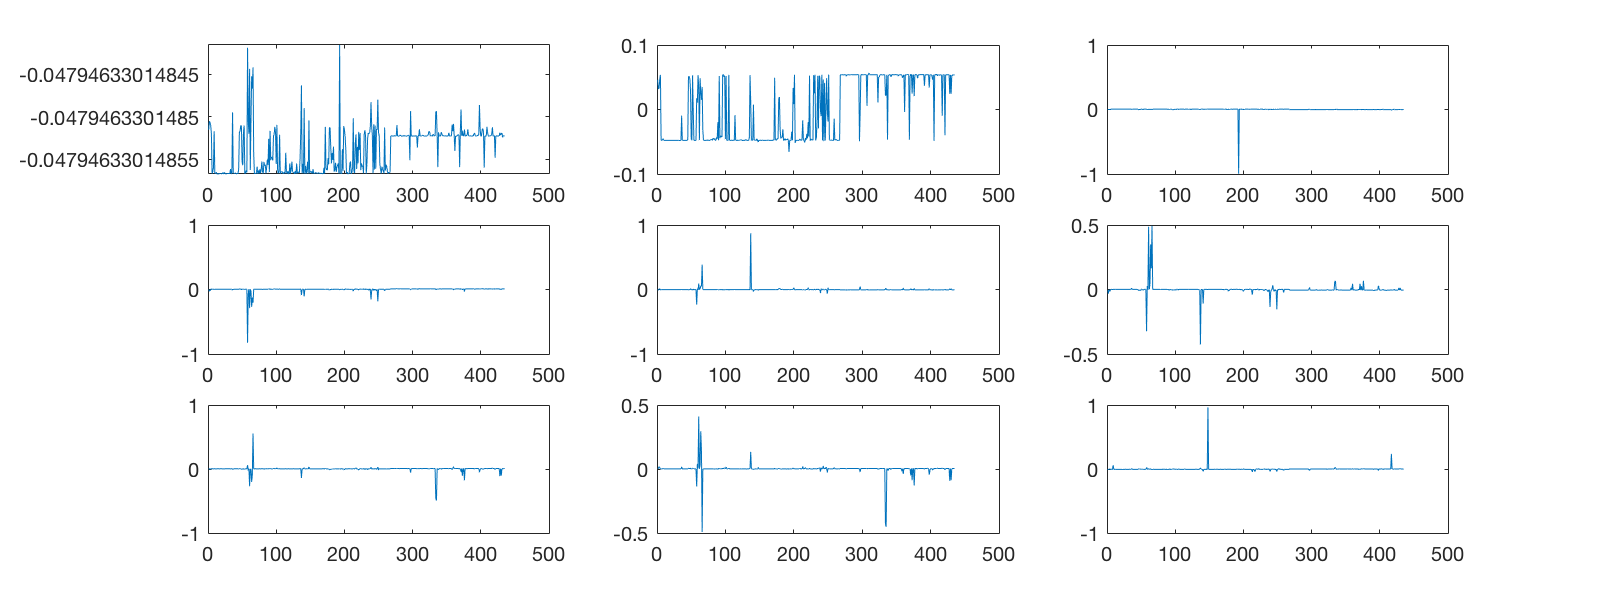
\includegraphics[width=\linewidth]{laplacians/voting_laplacian.png}
        \end{figure}

    \subsection{Two moons}
        This is a synthetic data set constructed with two half circles in $\mathbb{R}^2$ with radius one. These are embedded in $\mathbb{R}^{100}$, and data points are sampled from the circles with Gaussian noise distributed as $\mathsf{N}(0,\sigma^2)$ added to each of the 100 dimensions. In this data set, we will be generating realizations of two moons with $N=1000$ or $N=2000$ nodes, each associated with $d=100$ dimensional feature vectors. This data is again ordered, with the first $N/2$ nodes generated from the first half circle, and the latter $N/2$ from the second. Again, here we want to perform binary classification into the two half circles from which the data was generated. We will be using the self-tuning, symmetric Laplacian for this data set, introduced in \cite{SelfTuning}. This Laplacian matrix has weights that infer the local spatial scale from the data, removing the need to choose a fixed length-scale parameter. The use of this self-tuning Laplacian in the two-moons data set seems to encode more information in the eigenvectors. Compare \cref{fig:moon_spec} with \cref{fig:moon_un_spec}.

        \begin{figure}[!htb]
        \caption{\label{fig:moon_spec} Lowest $9$ eigenvectors of self-tuning symmetric $L$ of two moons, $\sigma = 0.04$.}
        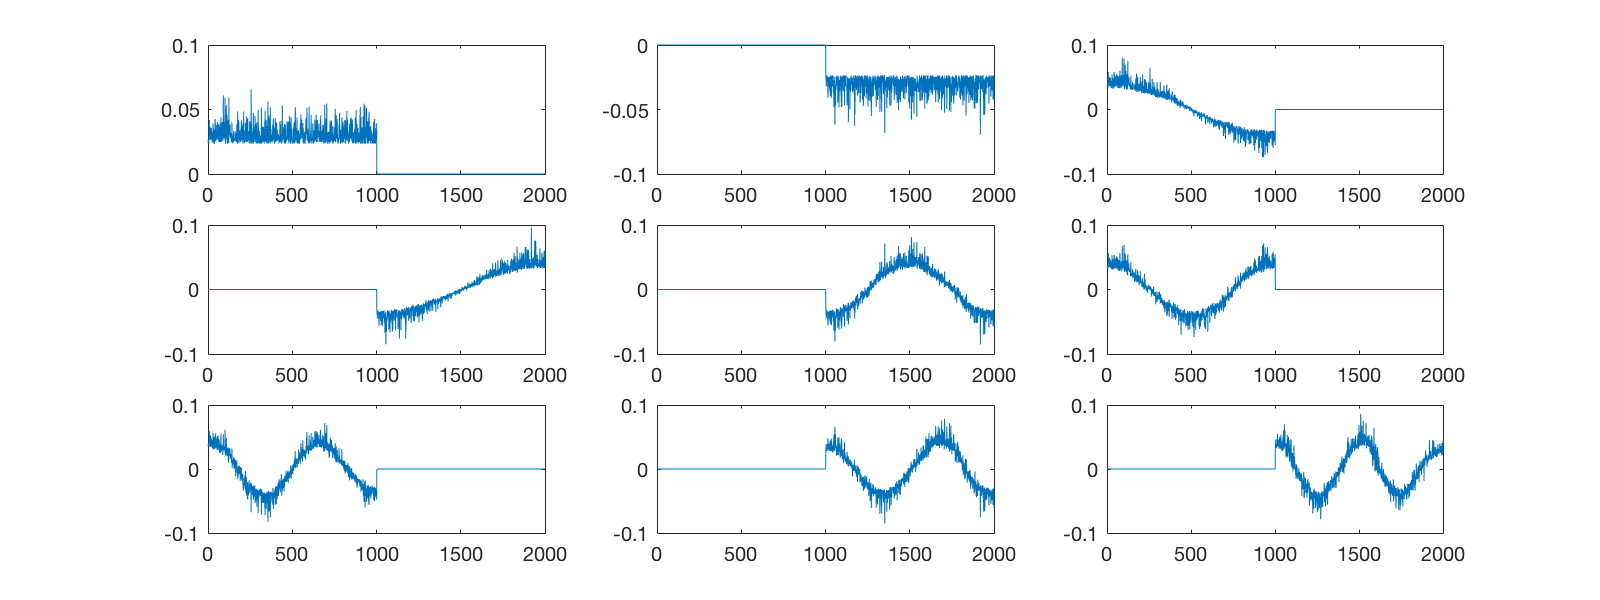
\includegraphics[width=\linewidth]{laplacians/moon_laplacian.png}
        \end{figure}

        \begin{figure}[!htb]
        \caption{\label{fig:moon_un_spec} Lowest $9$ eigenvectors of unnormalized fixed length $L$ of two moons, $\sigma = 0.04$.}
        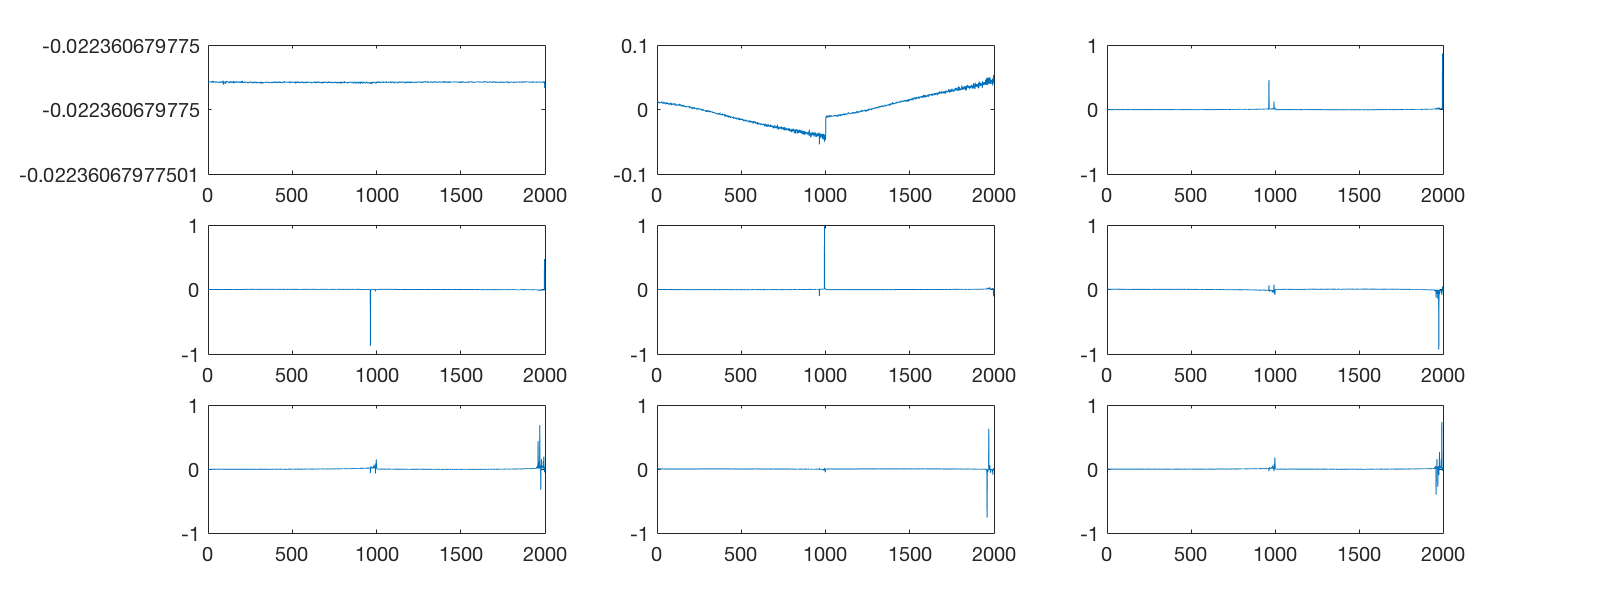
\includegraphics[width=\linewidth]{laplacians/moon_laplacian_un.png}
        \end{figure}

    \subsection{MNIST data sets}
        This data set contains 70,000 images of $28 \times 28$ pixels with handwritten digits $0$ through $9$. The feature vectors are $d=400$ dimensional and are formed by projection onto the first $50$ PCA components. We will focus on binary classification between the digits $4$ and $9$. We will use the self-tuning, symmetric normalized Laplacian again. See \cref{fig:mnist_spec}.

        \begin{figure}[!htb]
        \caption{\label{fig:mnist_spec} Lowest $9$ eigenvectors of self-tuning symmetric $L$ of MNIST, digits $4$ and $9$.}
        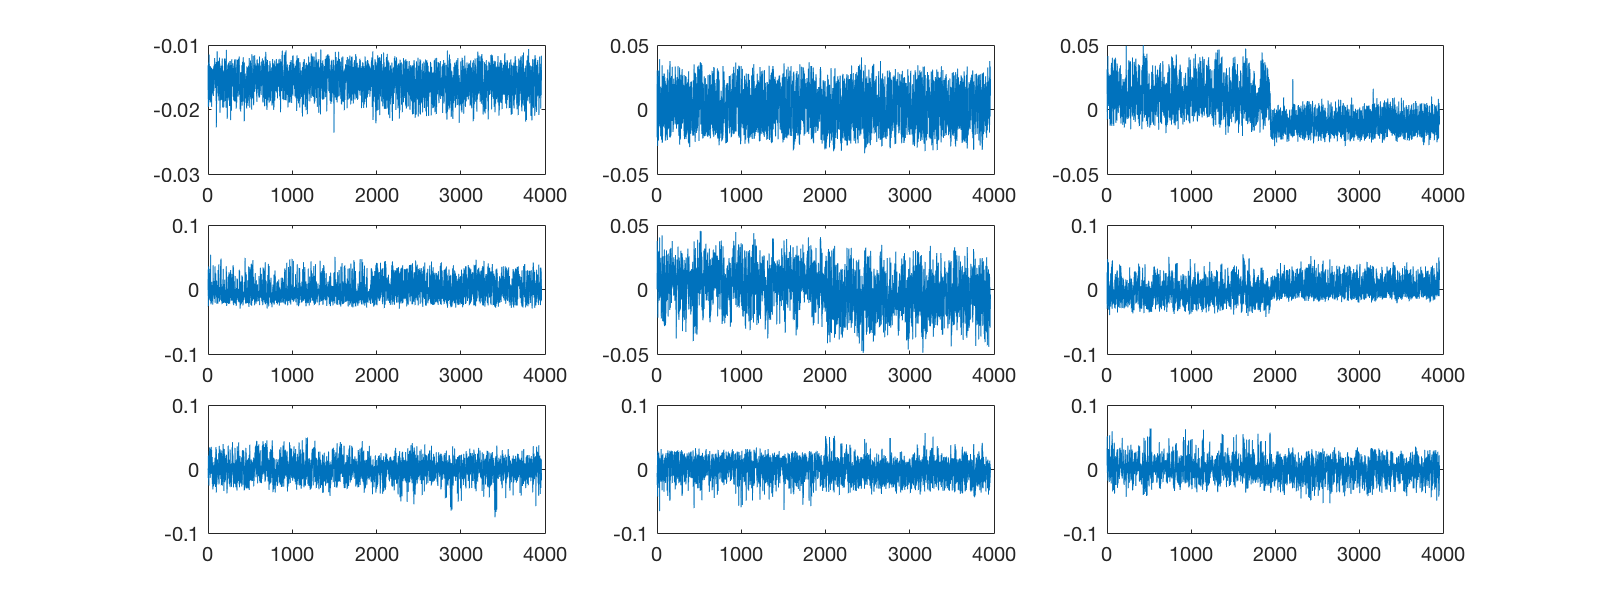
\includegraphics[width=\linewidth]{laplacians/mnist_laplacian.png}
        \end{figure}

\section{Algorithms}
    This section discusses the algorithms that I have implemented for the hierarchical models.

    \subsection{Model (A)}
        For the nonhierarchical model (A), I implemented a pCN algorithm first introduced in \cite{BeRoStVo08} and described in \cref{alg:generalpCN}.

        \begin{algorithm}
        \caption{General pCN adapted from \cite{CoRoStWh13}}
        \label{alg:generalpCN}
        \begin{algorithmic}[1]
        \State{Select $u^{(0)}$. Select $\tau, \alpha$. Select $\beta \in [0, 1]$}
        \For{$k = 0$ to $S$}
        \State{Sample $v$ from the prior distribution given in \cref{eqn:prior}}
        \State{Set $\hat u^{(k)} = (1- \beta^2)^{1/2}u^{(k)} + \beta v$}
        \State{Set $\alpha(u^{(k)} \to \hat u^{(k)}) = \min (1, \exp(\Phi(u^{(k)}) - \Phi(\hat u^{(k)})) )$}
        \State{Set $u^{(k+1)} = \hat u^{(k)}$ with probability $\alpha(u^{(k)} \to \hat u^{(k)})$, and set $u^{(k+1)} = u^{(k)}$ otherwise}
        \EndFor
        \State \Return $\{u^{(k)}\}$
        \end{algorithmic}
        \end{algorithm}

    \subsection{Model (B)}
        To implement model (B), which is hierarchical, we need to sample conditional distributions that govern $u, \tau,$ and $\alpha$. When we attempt to sample the posterior distribution in the hierarchical methods, we could use the Gibbs sampler. The basic form of Gibbs sampling has two repeated steps:
        \begin{itemize}
        \item Update $u^{(n+1)} \sim u|\theta^{(n)}, y$
        \item Update $\theta^{(n+1)} \sim \theta|u^{(n+1)}, y$
        \end{itemize}
        We use $\theta$ to represent the hyperparameters, which could include $\tau, \alpha,$ and $M$. However, we cannot sample the conditional distributions directly, so we replace direct sampling with Markov Chain Monte Carlo (MCMC) indirect sampling methods, which are invariant with respect to each of the exact conditional distributions. With Metropolis-within-Gibbs, at every step we update $u^{(n+1)}, \tau^{(n+1)}$ and $\alpha^{(n+1)}$ each with MCMC to target these conditional distributions. One method is to update $u, \tau, \alpha$ in a block, by proposing $(u,\theta) \to  (\hat u, \hat \theta)$ and computing the transition probability for this step. 

        The algorithms that we will implement will be slightly different, as we will independently propose $u \to \hat u, \tau \to \hat \tau, \alpha \to \hat \alpha, M \to \hat M$, and perform these transitions in separate steps. At each step, we fix all but the proposed parameter, and we compute the transition probability. This is the algorithm that we will be using for the following hierarchical algorithms.

        Our first of two hierarchical algorithms for model (B) is deemed ``centered," as contrasted with the second algorithm described later in this section. Using Metropolis-within-Gibbs, we will require an expression for the posterior, so define $f(u,\tau,\alpha)$ as the joint posterior distribution. By Bayes' theorem, 
        \[f(u,\tau,\alpha) \propto \exp(-\Phi(u))\times\mathbb{P}(u,\tau,\alpha) = \exp(-\Phi(u))\mathbb{P}(u|\theta)\pi_0(\theta).\]
        Recall from \cref{eqn:prior} that the prior is distributed as $\mathsf{N}(0, C)$ with the covariance matrix $C(\theta) = C(\tau, \alpha) = (L + \tau^2I)^{-\alpha}$. We can write

        \begin{equation}
        \label{eqn:centered_post}
        f(u,\tau,\alpha) \propto 
        \frac{1}{\sqrt{(2\pi)^d \det C(\tau,\alpha)}} \exp\left(-\Phi(u)-\frac{1}{2}\langle u, C(\tau,\alpha)^{-1}u  \rangle + \log(\pi_0(\tau,\alpha)) \right).
        \end{equation}
        The normalization constant $\det(C(\theta))$ depends on $\tau, \alpha$ now and does not cancel out. Using this expression for the posterior, I implemented the Metropolis-within-Gibbs method for model (B) in \cref{alg:hierarchical_tau_alpha}.

        \begin{algorithm}
        \caption{Hierarchical on $\tau, \alpha$}
        \label{alg:hierarchical_tau_alpha}
        \begin{algorithmic}[1]
        \State Initialize $u^{(0)} = q_1$, the Fiedler vector expressed in the standard basis.
        \State Initialize $\tau^{(0)}, \alpha^{(0)}$. Select $\beta \in [0, 1]$
        \State Pick $\epsilon_1, \epsilon_2$, the jump sizes for $\tau, \alpha$ respectively.
        \For{$k = 0$ to $S$}
        \State Sample $v$ from the prior distribution and expressed in the eigenbasis \Comment{$u|y, \tau, \alpha$}.
        \State Expressing $u$ in the eigenbasis, set a proposal $\hat u^{(k)} = (1- \beta^2)^{1/2}u^{(k)} + \beta v$
        \State Set $u^{(k+1)} = \hat u^{(k)}$ with probability 
        \[A(u^{(k)} \to \hat u^{(k)}) = \min \left\{1, \exp(\Phi(u^{(k)}) - \Phi(\hat u^{(k)})) \right\}\]

        \State Set a proposal $\hat \tau^{(k)} = \tau^{(k)} + \epsilon_1 t$ for $t \sim \mathsf{N}(0, 1)$ \Comment{$\tau|y,u,\alpha$}
        \State Set $\tau^{(k+1)} = \hat \tau^{(k)}$ with probability 

        \[A(\tau^{(k)} \to \hat \tau^{(k)}) = \min \left\{ 1, \frac{f(u^{(k+1)}, \hat \tau^{(k)}, \alpha^{(k)})}{f(u^{(k+1)}, \tau^{(k)}, \alpha^{(k)})}\right\}\]
        (Using the eigenbasis representation of $u$ for computation) \Comment{$f$ defined in \cref{eqn:centered_post}}

        \State Set a proposal $\hat \alpha^{(k)} = \alpha^{(k)} + \epsilon_2 a$ for $a \sim \mathsf{N}(0, 1)$ \Comment{$\alpha|y,u,\tau$}
        \State Set $\alpha^{(k+1)} = \hat \alpha^{(k)}$ with probability

         \[A(\alpha^{(k)}\to\hat\alpha^{(k)}) = 
         \min\left\{1, 
         \frac{f(u^{(k+1)}, \tau^{(k+1)}, \hat \alpha^{(k)})}
         {f(u^{(k+1)}, \tau^{(k+1)}, \alpha^{(k)})}\right\}
         \]

        \EndFor
        \State \Return $\{u^{(k)}, \tau^{(k)}, \alpha^{(k)}\}$
        \end{algorithmic}
        \end{algorithm}



        We also looked at a different parameterization for model (B). \cref{alg:xi_tau_alpha} uses the variable $\xi$ that is related to the classifying function $u$ by 
        \begin{equation}
        \label{eqn:noncentered_T}
        T(\xi,\tau,\alpha) = \sum_{i=0}^M \frac{1}{(\lambda_i+\tau^2)^{\alpha/2}}\xi_iq_i = u
        \end{equation}

        following \cref{eqn:prior}. This algorithm is ``non-centered" compared to the centered parameterization given in \cref{alg:hierarchical_tau_alpha}, meaning that the unknown classifying variable $\xi$ and the parameters $\theta=(\tau,\alpha)$ are a priori independent \cite{Noncentered}.

        This model assumes the prior $\xi \sim \mathsf{N}(0,I)$. Similar to the centered case, define $g(\xi,\tau,\alpha)$ as the joint posterior distribution. By Bayes' theorem, 
        \[g(\xi,\tau,\alpha) \propto \exp(-\Phi(T(\xi,\tau,\alpha)))\times \mathbb{P}(\xi,\tau,\alpha) = \exp(-\Phi(T(\xi,\tau,\alpha)))\mathbb{P}(\xi)\pi_0(\tau, \alpha).\]
        Note that $\mathbb{P}(\xi) = \frac{1}{\sqrt{(2\pi)^d \det I}} \exp(-\frac{1}{2}\langle \xi, I\xi  \rangle) \propto \exp(-\frac{1}{2}\langle \xi,\xi \rangle)$ and the normalization constants drop out. We obtain:
        \begin{equation}
        \label{eqn:noncentered_post}
        g(\xi,\tau,\alpha) \propto \exp\left( -\Phi(T(\xi,\tau,\alpha))-\frac{1}{2}\langle \xi,\xi \rangle + \log(\pi_0(\tau,\alpha)) \right).
        \end{equation}

        \begin{algorithm}
        \caption{Non-centered parameterization: sampling $\xi, \tau, \alpha$}
        \label{alg:xi_tau_alpha}
        \begin{algorithmic}[1]
        \State Choose $\xi^{(0)} \in \mathbb{R}^N, \alpha^{(0)}, \tau^{(0)} > 0, \beta \in (0, 1]$ and $\epsilon_1, \epsilon_2 > 0$.
        \For{$k=0$ to $S$}
        \State Propose $\hat\xi^{(k)} = (1-\beta^2)^{\frac{1}{2}}\xi^{(k)} + \beta \zeta^{(k)}$, $\zeta^{(k)} \sim \mathsf{N}(0, I)$
        \State Make transition $\xi^{(k)} \to \hat\xi^{(k)}$ with probability
        \[ A(\xi^{(k)} \to \hat\xi^{(k)}) = \min\left\{1, \exp\left(\Phi(T(\xi^{(k)},\tau^{(k)},\alpha^{(k)})) - \Phi(T(\hat\xi^{(k)},\tau^{(k)},\alpha^{(k)}))\right) \right\}\] \Comment{$T$ defined in \cref{eqn:noncentered_T}}

        \State Propose $\hat\tau^{(k)} = \tau^{(k)} + \epsilon_1 \rho^{(k)}, \rho^{(k)} \sim \mathsf{N}(0,1)$
        \State Make transition $\tau^{(k)} \to \hat\tau^{(k)}$ with probability
        \[ A(\tau^{(k)} \to \hat\tau^{(k)}) = \min\left\{1, \frac{g(\xi^{(k+1)},\hat\tau^{(k)},\alpha^{(k)})}{g(\xi^{(k+1)},\tau^{(k)},\alpha^{(k)})} \right\}\] \Comment{$g$ defined in \cref{eqn:noncentered_post}}

        \State Propose $\hat\alpha^{(k)} = \alpha^{(k)} + \epsilon_2 \sigma^{(k)}, \sigma^{(k)} \sim \mathsf{N}(0,1)$
        \State Make transition $\alpha^{(k)} \to \hat\alpha^{(k)}$ with probability
        \[ A(\alpha^{(k)} \to \hat\alpha^{(k)}) = \min\left\{1, \frac{g(\xi^{(k+1)},\tau^{(k+1)},\hat \alpha^{(k)})}{g(\xi^{(k+1)},\tau^{(k+1)},\alpha^{(k)})} \right\}\]
        \EndFor
        \State \Return $\{ T(\xi^{(k)},\tau^{(k)},\alpha^{(k)}), \tau^{(k)}, \alpha^{k} \}$
        \end{algorithmic}
        \end{algorithm}

    \subsection{Model (C)}
        In this algorithm, we aim to learn $M$, the number of eigenvectors we want to use, as well. This algorithm seems promising given the problem we encountered with the irregularity of higher eigenvectors with the algorithms in model (B), which we resolved by truncating the number of eigenvectors. Essentially, we want to be hierarchical about our level of truncation. We take a uniform prior for $M$, typically $\mathsf{U}(1,70)$ or similar. It is convenient to implement this algorithm with the non-centered approach since we do not need to worry about $M$ affecting terms such as the determinant of the covariance. The new equation for $T$, which relates $\xi, \tau, \alpha, M$ to $u$, is:
        \begin{equation}
            \label{eqn:noncentered_T_M}
            T(\xi,\tau,\alpha, M) = \sum_{i=0}^M \frac{1}{(\lambda_i+\tau^2)^{\alpha/2}}\xi_iq_i = u.
        \end{equation}

        We can compute the joint posterior on $\xi, \tau, \alpha, M$ similarly to the derivation of \cref{eqn:noncentered_post}:

        \begin{equation}
        \label{eqn:noncentered_post_M}
        g(\xi,\tau,\alpha, M) \propto \exp\left( -\Phi(T(\xi,\tau,\alpha,M))-\frac{1}{2}\langle \xi,\xi \rangle + \log(\pi_0(\tau,\alpha,M)) \right).
        \end{equation}

        The only modification from \cref{alg:xi_tau_alpha} is to add a random walk proposal for $M$ and compute the acceptance probability as the ratio of the joint posteriors. This algorithm is given in \cref{alg:hier_t_a_M}.

        \begin{algorithm}

        \caption{Non-centered parameterization, hierarchical with $\tau, \alpha, M$}
        \label{alg:hier_t_a_M}
        \begin{algorithmic}[1]
        \State Choose $\xi^{(0)} \in \mathbb{R}^N, \tau^{(0)}, \alpha^{(0)}, M^{(0)} > 0, \beta \in (0, 1]$ and $\epsilon_1, \epsilon_2 > 0$.
        \For{$k=0$ to $S$}
        \State Propose $\hat\xi^{(k)} = (1-\beta^2)^{\frac{1}{2}}\xi^{(k)} + \beta \zeta^{(k)}$, $\zeta^{(k)} \sim \mathsf{N}(0, I)$
        \State Make transition $\xi^{(k)} \to \hat\xi^{(k)}$ with probability
        \[ A(\xi^{(k)} \to \hat\xi^{(k)}) = \min\left\{1, \exp\left(\Phi(T(\xi^{(k)},\tau^{(k)},\alpha^{(k)}, M^{(k)})) - \Phi(T(\hat\xi^{(k)},\tau^{(k)},\alpha^{(k)}, M^{(k)}))\right) \right\}\] \Comment{$T$ defined in \cref{eqn:noncentered_T_M}}

        \State Propose $\hat\tau^{(k)} = \tau^{(k)} + \epsilon_1 \rho^{(k)}, \rho^{(k)} \sim \mathsf{N}(0,1)$
        \State Make transition $\tau^{(k)} \to \hat\tau^{(k)}$ with probability
        \[ A(\tau^{(k)} \to \hat\tau^{(k)}) 
        = \min\left\{1, \frac{g(\xi^{(k+1)},\hat\tau^{(k)},\alpha^{(k)},M^{(k)})}{g(\xi^{(k+1)},\tau^{(k)},\alpha^{(k)},M^{(k)})} \right\}\] \Comment{$g$ defined in \cref{eqn:noncentered_post_M}}

        \State Propose $\hat\alpha^{(k)} = \alpha^{(k)} + \epsilon_2 \sigma^{(k)}, \sigma^{(k)} \sim \mathsf{N}(0,1)$
        \State Make transition $\alpha^{(k)} \to \hat\alpha^{(k)}$ with probability
        \[ A(\alpha^{(k)} \to \hat\alpha^{(k)}) 
        = \min\left\{1, \frac{g(\xi^{(k+1)},\tau^{(k+1)},\hat \alpha^{(k)},M^{(k)})}{g(\xi^{(k+1)},\tau^{(k+1)},\alpha^{(k)},M^{(k)})} \right\}\]
        \State Propose $\hat M^{(k)} = M^{(k)} + Q$, with jump $Q$ distributed as $\mathbb{P}(Q=k) \propto \frac{1}{1+|k|}$, $|Q|$ bounded.
        \State Make transition $M^{(k)} \to \hat M^{(k)}$ with probability
        \[ A(M^{(k)} \to \hat M^{(k)}) = 
        \min\left\{1, \frac{g(\xi^{(k+1)},\tau^{(k+1)},\alpha^{(k+1)},\hat M^{(k)})}{g(\xi^{(k+1)},\tau^{(k+1)},\alpha^{(k+1)},M^{(k)})} \right\}
        \]
        \EndFor
        \State \Return $\{ T(\xi^{(k)},\tau^{(k)},\alpha^{(k)}, M^{(k)}), \tau^{(k)}, \alpha^{k} \}$
        \end{algorithmic}
        \end{algorithm}

    \subsection{Model (D)} \label{sec:algorithms_model_d}
        This algorithm reparameterizes the problem in terms of the random vectors $v$ and $\xi$. $v_j$ modifies the scale of influence of $q_j$, the $j$th eigenvector of the graph Laplacian, on the classifying function $u$.
        \begin{equation}
        \label{eqn:v_T}
        T(v,\xi) = \sum_{i=0}^{M} v_i\xi_iq_i = u.
        \end{equation}
        Here, $M$ is fixed. We take $\xi \sim \mathsf{N}(0, I)$. Using good estimates for $\tau, \alpha$, perhaps obtained by algorithms that learn $\tau, \alpha$, set the prior on $v$ to be:
        \[v_j \sim \mathsf{U}\left((1-a)(\lambda_j+\tau^2)^{-\alpha/2},(1+a)(\lambda_j+\tau^2)^{-\alpha/2}\right)\]
        where $a$ is a fixed scalar.

        Finally, we derive an expression for the posterior with Bayes' theorem.
        \begin{align*}
        \mathbb{P}(v,\xi | y) &\propto \mathbb{P}(y|v, \xi) \mathbb{P}(v, \xi)\\
        &\propto \exp \left(-\Phi(T(v,\xi)) \right) \mathbb{P}(v)\mathbb{P}(\xi) \\
        &\propto \exp \left(-\Phi(T(v,\xi)) + \log (\pi_0(v)) - \frac{1}{2}\langle \xi, \xi \rangle  \right).
        \end{align*}

        Let $h(v,\xi)$ denote the joint posterior on $v$ and $\xi$. Then,
        \begin{equation}
        \label{eqn:learn_v_posterior}
        h(v, \xi) \propto \exp \left(-\Phi(T(v,\xi)) + \log (\pi_0(v)) - \frac{1}{2}\langle \xi, \xi \rangle  \right).
        \end{equation}

        The updates for this algorithm will be done as follows:

        \begin{itemize}
            \item Update $\xi^{(k+1)} | v^{(k)}, y$ with a pCN proposal.
            \item Update $v^{(k+1)} | \xi^{(k+1)}, y$ with a random walk on the uniform prior for $v$.
        \end{itemize}

        This algorithm is given in \cref{alg:hier_v}.
        \begin{algorithm}
            \caption{Non-centered parameterization, hierarchical with $v$}
            \label{alg:hier_v}
            \begin{algorithmic}[1]
            \State Choose $v^{(0)}, \xi^{(0)} \in \mathbb{R}^N, \beta \in (0, 1], \epsilon > 0$.
            \For{$k=0$ to $S$}
            \State Propose $\hat\xi^{(k)} = (1-\beta^2)^{\frac{1}{2}}\xi^{(k)} + \beta \zeta^{(k)}$, $\zeta^{(k)} \sim \mathsf{N}(0, I)$
            \State Make transition $\xi^{(k)} \to \hat\xi^{(k)}$ with probability
            \[ A(\xi^{(k)} \to \hat\xi^{(k)}) = \min\left\{1, \exp\left(\Phi(T(v^{(k)}, \xi^{(k)})) - \Phi(T(v^{(k)}, \hat \xi^{(k)}))\right) \right\}\]

            \State Propose $\hat v^{(k)} = v^{(k)} + \epsilon \rho^{(k)}, \rho^{(k)} \sim \mathsf{N}(0,I)$
            \If {$\hat v^{(k)} _j$ is outside of its prior interval for any $j$} 
                \State Reject and set $v^{(k+1)} = v^{(k)}$.
            \Else
            \State Make transition $v^{(k)} \to \hat v^{(k)}$ with probability
            \begin{align*}
             A(v^{(k)} \to \hat v^{(k)}) &= \min\left\{1, \frac{h(\hat v^{(k)}, \xi^{(k+1)})}{h(v^{(k)}, \xi^{(k+1)})}\right\} \\
             &= \min\left\{1, \exp\left(\Phi(T(v^{(k)}, \xi^{(k+1)}))-\Phi(T(\hat v^{(k)}, \xi^{(k+1)})) \right) \right\}
             \end{align*}
            \EndIf

            \EndFor
            \State \Return $\{ T(v^{(k)},\xi^{(k)}), v^{(k)}, \xi^{(k)} \}$
            \end{algorithmic}
        \end{algorithm}

    \subsection{Model (E)} \label{sec:algorithms_model_e}
        This model extends model (D), trying to learn $M$ as well. Define:
        \begin{equation}
        T(v,\xi,M) = \sum_{i=0}^{M} v_i\xi_iq_i = u.
        \end{equation}
        Taking the uniform prior on $v$, we obtain:
        \begin{equation}
        \label{eqn:learn_v_M_posterior}
        h(v, \xi, M) \propto \exp \left(-\Phi(T(v,\xi, M)) + \log (\pi_0(v, M)) - \frac{1}{2}\langle \xi, \xi \rangle  \right).
        \end{equation}
        This approach is described in \cref{alg:hier_v_M}.
        \begin{algorithm}
        \caption{Non-centered parameterization, hierarchical with $v, M$}
        \label{alg:hier_v_M}
        \begin{algorithmic}[1]
        \State Choose $v^{(0)}, \xi^{(0)} \in \mathbb{R}^N, M^{(0)}, \beta \in (0, 1], \epsilon > 0$.
        \For{$k=0$ to $S$}
        \State Propose $\hat\xi^{(k)} = (1-\beta^2)^{\frac{1}{2}}\xi^{(k)} + \beta \zeta^{(k)}$, $\zeta^{(k)} \sim \mathsf{N}(0, I)$
        \State Make transition $\xi^{(k)} \to \hat\xi^{(k)}$ with probability
        \[ A(\xi^{(k)} \to \hat\xi^{(k)}) = \min\left\{1, \exp\left(\Phi(T(v^{(k)}, \xi^{(k)}, M^{(k)})) - \Phi(T(v^{(k)}, \hat \xi^{(k)}, M^{(k)}))\right) \right\}\]

        \State Propose $\hat v^{(k)} = v^{(k)} + \epsilon \rho^{(k)}, \rho^{(k)} \sim \mathsf{N}(0,I)$
        \If {$\hat v^{(k)} _j$ is outside of its prior interval for any $j$} 
            \State Reject and set $v^{(k+1)} = v^{(k)}$.
        \Else
        \State Make transition $v^{(k)} \to \hat v^{(k)}$ with probability
        \begin{align*}
         A(v^{(k)} \to \hat v^{(k)}) &= \min\left\{1, \frac{h(\hat v^{(k)}, \xi^{(k+1)}, M^{(k)})}{h(v^{(k)}, \xi^{(k+1)}, M^{(k)})}\right\} \\
         &= \min\left\{1, \exp\left(\Phi(T(v^{(k)}, \xi^{(k+1)},M^{(k)}))-\Phi(T(\hat v^{(k)}, \xi^{(k+1)}, M^{(k)})) \right) \right\}
         \end{align*}
        \EndIf

        \State Propose $\hat M^{(k)} = M^{(k)} + Q$, with jump $Q$ distributed as $\mathbb{P}(Q=k) \propto \frac{1}{1+|k|}$, $|Q|$ bounded.
        \State Make transition $M^{(k)} \to \hat M^{(k)}$ with probability

        \begin{align*}
        A(M^{(k)} \to \hat M^{(k)}) &= \min\left\{1, \frac{h( v^{(k+1)}, \xi^{(k+1)}, \hat M^{(k)}  )}{h( v^{(k+1)}, \xi^{(k+1)}, M^{(k)} )} \right\}\\
        &=\min\left\{1, \exp\left(\Phi(v^{(k+1)}, \xi^{(k+1)}, M^{(k)} ) - \Phi(v^{(k+1)}, \xi^{(k+1)}, \hat M^{(k)} )\right)\right\}
        \end{align*}

        \EndFor
        \State \Return $\{ T(v^{(k)},\xi^{(k)}), v^{(k)}, \xi^{(k)} \}$
        \end{algorithmic}
        \end{algorithm}

    \subsection{Multiclass} \label{sec:algorithms_multiclass}
        We describe the algorithm to solve the multiclass clustering problem. Recall that for $v \in \mathbb{R}^k$, we define $S(v) = e_p, \quad p = \text{argmax} (v_r)$ where $\{e_1, \ldots e_k\}$ is the standard basis of $\mathbb{R}^k$. Now, the classifying function is of the form $u: Z \to \mathbb{R}^k$, or $u = (u^{[1]}, u^{[2]}, \ldots u^{[k]})$ with functions $u^{[j]}: Z \to \mathbb{R}$. Each of the $u^{[j]}$ has prior distribution given by $\mathsf{N}(0, C)$ with $C = (L + \tau^2 I)^{-\alpha}$. We retain
        \[ \Phi(u) = \frac{1}{2\gamma^2}\sum_{l \in Z'} \text{norm}(y(l) - S(u(l)))^2. \]

        We will implement the non-centered approach. Here, the variable is $\xi = (\xi^{[1]}, \ldots \xi^{[k]})$ where each $\xi^{[j]}$ is associated with $u^{[j]}$ by the following:
        \[T(\xi^{[j]}) = \sum_{i=1}^M \frac{1}{(\lambda_j + \tau^2)^{\alpha/2}} \xi^{[j]}_i q_i = u^{[j]}.\]
        Then, define:
        \begin{equation}
        \label{eqn:multiclass_T}
        T(\xi) = (T(\xi^{[1]}), \ldots T(\xi^{[k]}) ) = u.
        \end{equation}

        Refer to \cref{alg:multiclass_nonhier}.
        
        \begin{algorithm}

        \caption{Multiclass, Metropolis-within-Gibbs updates}
        \label{alg:multiclass_nonhier}
        \begin{algorithmic}[1]
        \State Choose $\xi^{(0)} = (\xi^{[1],(0)}, \ldots \xi^{[k],(0)}), \xi^{[j],(0)} \in \mathbb{R}^M$. Choose $\tau, \alpha, \beta \in (0, 1]$. \Comment{We refer to $\xi^{[j],(i)}$ as the $i$th observation of $\xi^{[j]}$.}
        \For{$i=0$ to $S$}
            \For{$j=1$ to $k$}
                \State Propose $\hat\xi^{[j],(i)} = (1-\beta^2)^{\frac{1}{2}}\xi^{[j],(i)} + \beta \zeta^{(i)}$, $\zeta^{(i)} \sim \mathsf{N}(0, I)$
                \State Define $\hat \xi = (\xi^{[1],(i+1)}, \ldots \xi^{[j-1],(i+1)}, \hat\xi^{[j],(i)}, \xi^{[j+1],(i)}, \ldots)$
                \State Make transition $\xi^{(i)} \to \hat\xi$ with probability
                \[ A(\xi^{(i)} \to \hat\xi) = \min\left\{1, \exp\left(\Phi(T(\xi^{(i)})) - \Phi(T(\hat \xi))\right) \right\}\]

            \EndFor
        \EndFor

        \State \Return $\{T(\xi^{(i)})\}$
        
        \end{algorithmic}
        \end{algorithm}

        We can extend this algorithm to be hierarchical with $\tau, \alpha, M$ as in the binary case. Define $T$ as
         \[T(\xi^{[j]}, \tau, \alpha, M) = \sum_{i=1}^M \frac{1}{(\lambda_j + \tau^2)^{\alpha/2}} \xi^{[j]}_i q_i = u^{[j]}.\]
         One choice we have to make is whether there should be one universal copy of $\tau, \alpha, M$ for all of the $k$ copies of the prior, or if each copy should have its own independently-evolving hyperparameters.
\iffalse

\section{Voting records experiments with models (A) and (B)}
    In each of the following experiments, the labeled data $Z'$ was chosen consistently: members 20-30 was labeled one party and members 280-290 as the other.

    For \cref{alg:generalpCN}, fixing $\gamma = 0.0001, \beta = 0.4, \tau = 1, \alpha = 1$, and running for $100000$ iterations with a burn-in period of $1000$, I could get clustering at about 85\% accuracy. One final clustering obtained is shown in \cref{fig:mcmc_gamma_final}, with relevant figures \cref{fig:mcmc_gamma_acceptance} and \cref{fig:mcmc_gamma_senators} that suggest that the chain has converged.
    \begin{figure}[!htb]
    \begin{minipage}{0.48\textwidth}
        \caption{\label{fig:mcmc_gamma_final} \cref{alg:generalpCN} final average}
        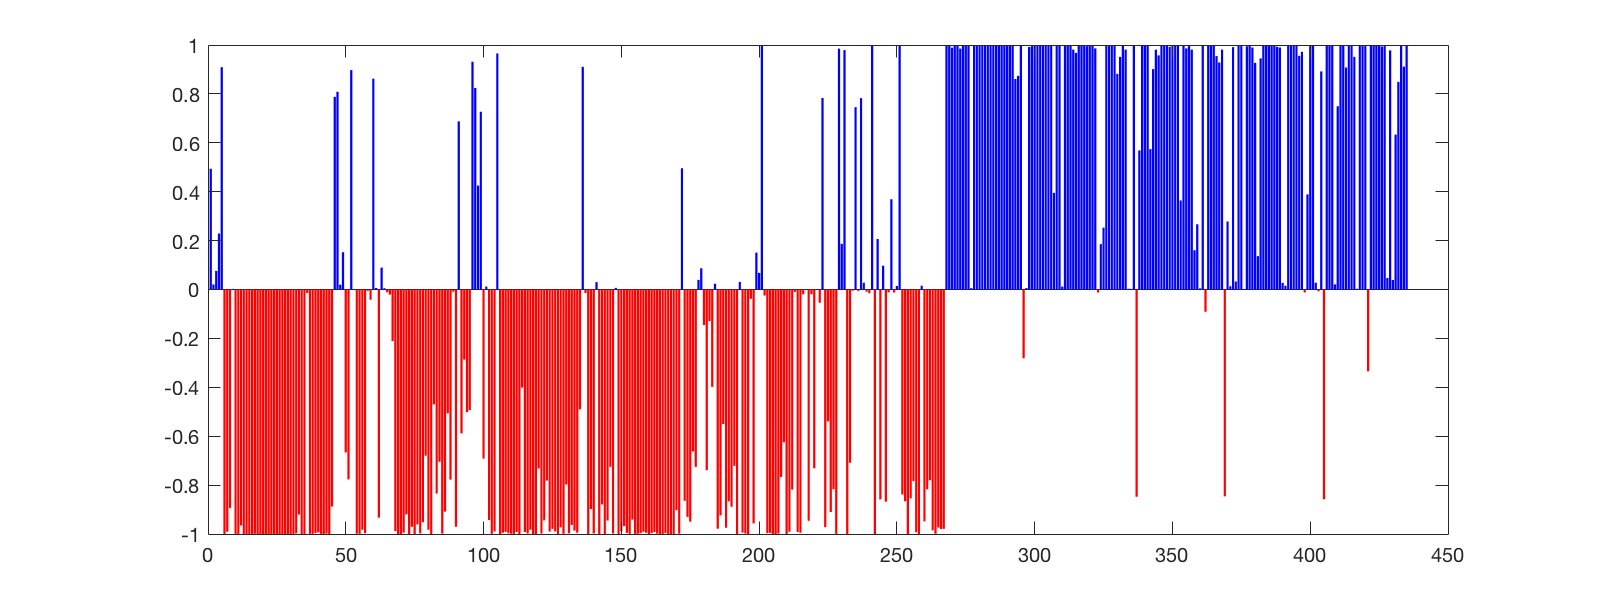
\includegraphics[width = \linewidth]{voting/mcmc_gamma/final_avg.png}
    \end{minipage}\hfill
    \begin{minipage}{0.48\textwidth}
        \caption{\label{fig:mcmc_gamma_acceptance} \cref{alg:generalpCN} average $u$ acceptance probability}
        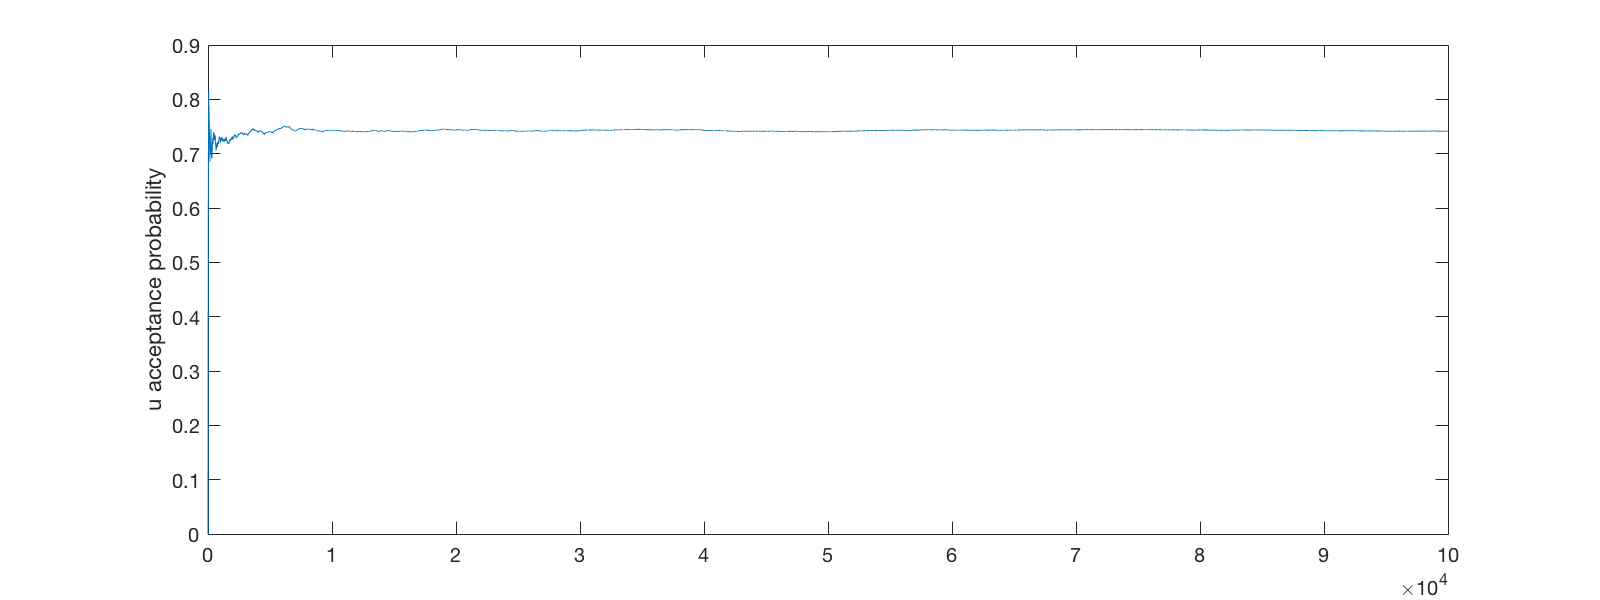
\includegraphics[width=\linewidth]{voting/mcmc_gamma/u_accept.png}
    \end{minipage}
    \end{figure}

    \begin{figure}[!htb]
    \caption{\label{fig:mcmc_gamma_senators} Running averages of classifications of delegates}
    \centering
    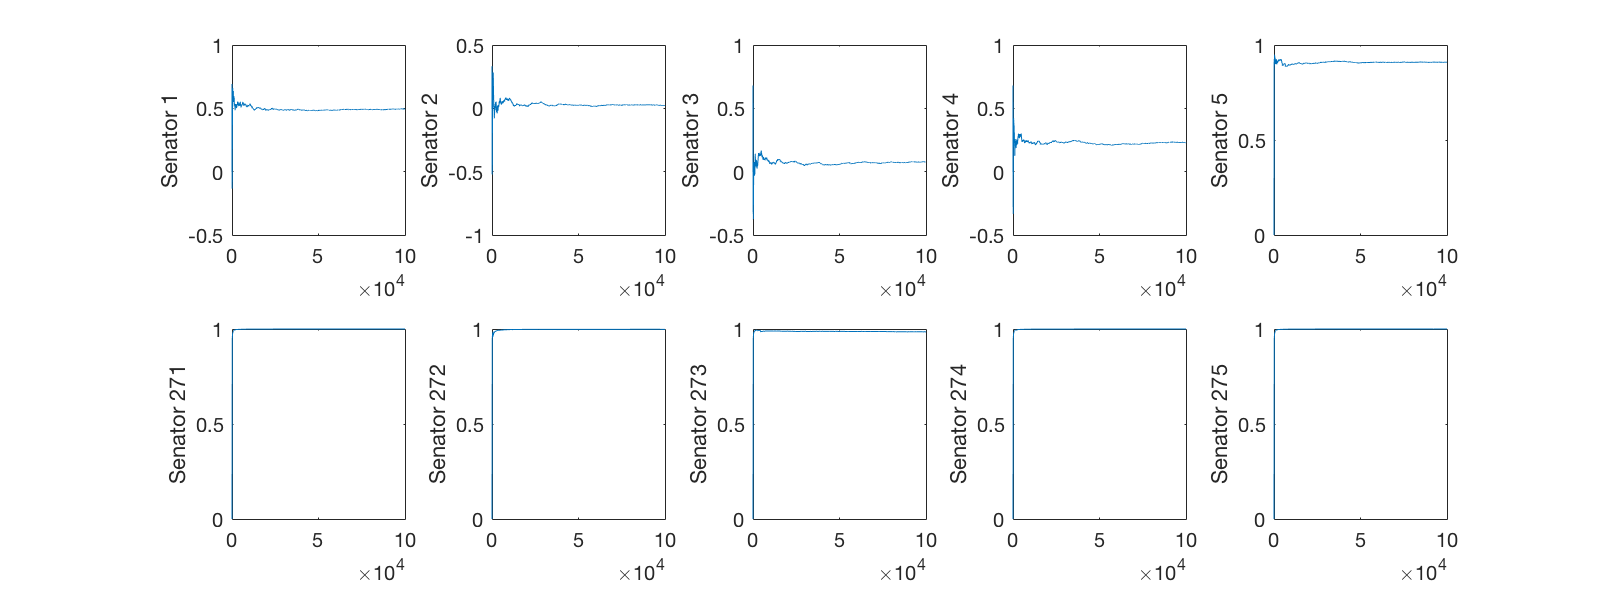
\includegraphics[width=\linewidth]{voting/mcmc_gamma/senator_avgs.png}
    \end{figure}
    Experiments with \cref{alg:hierarchical_tau_alpha} on the voting records data indicated poor mixing in the hyperparameters by looking at traces of $\tau, \alpha$. We decided that the problem was in part due to the irregularity of the larger eigenvectors, perhaps because of the accuracy of MATLAB's eig solver. Truncating the list of eigenvectors to only consider the first 50 seemed to help the problem, and we were able to observe better clustering. Fixing $\gamma = 0.0001, \beta = 0.4, \tau^{(0)}=20,\alpha^{(0)}=20,\tau\in[0.1,60],\alpha\in[0.1,60],\epsilon_\tau=0.1,\epsilon_\alpha=0.1$ and running $100000$ iterations with a burn-in period of $1000$, the accuracy is about 83\%. See \cref{fig:centered_voting_avg}, \cref{fig:centered_voting_accept}, \cref{fig:centered_voting_tau}, \cref{fig:centered_voting_alpha}.

    \begin{figure}[!htb]
    \begin{minipage}{0.48\textwidth}
        \caption{\label{fig:centered_voting_avg} \cref{alg:hierarchical_tau_alpha} after truncating eigenvectors, final average}
        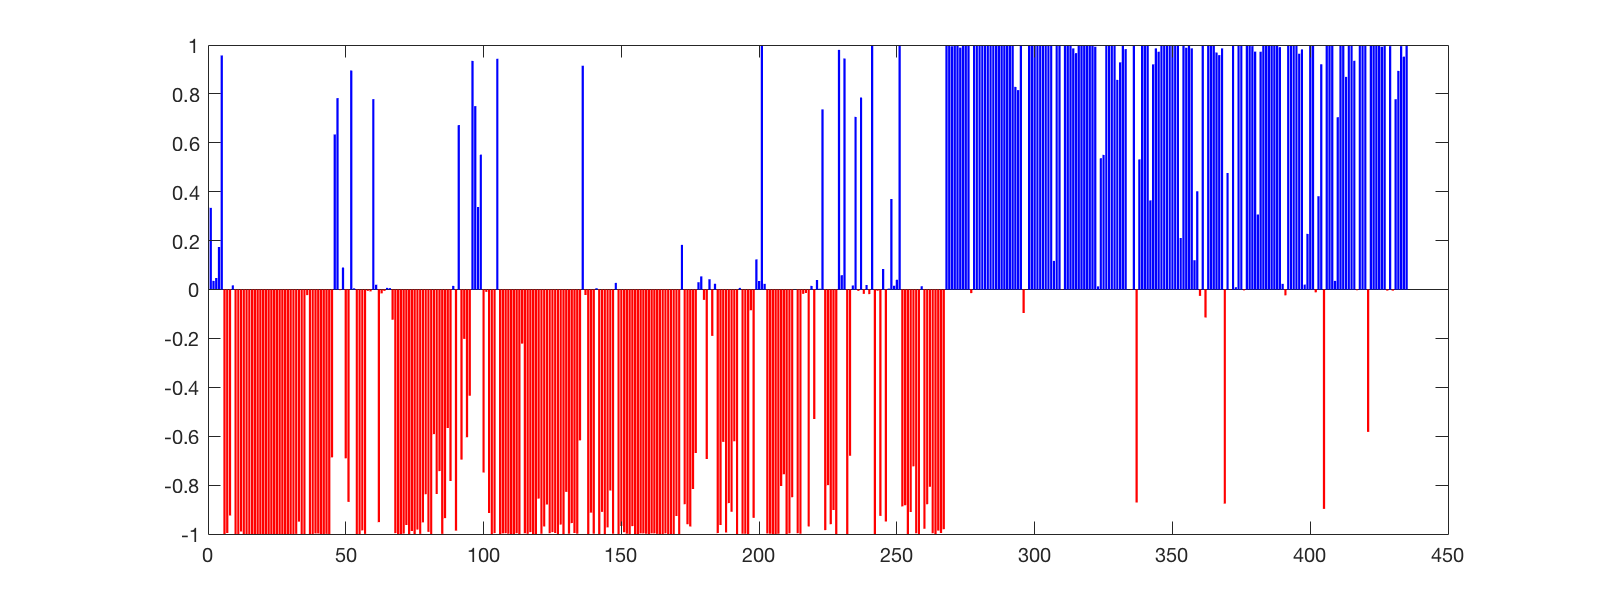
\includegraphics[width=\linewidth]{voting/centered/final_avg.png}
    \end{minipage}\hfill
    \begin{minipage}{0.48\textwidth}
        \caption{\label{fig:centered_voting_accept} \cref{alg:hierarchical_tau_alpha} average $u$ acceptance probability}
        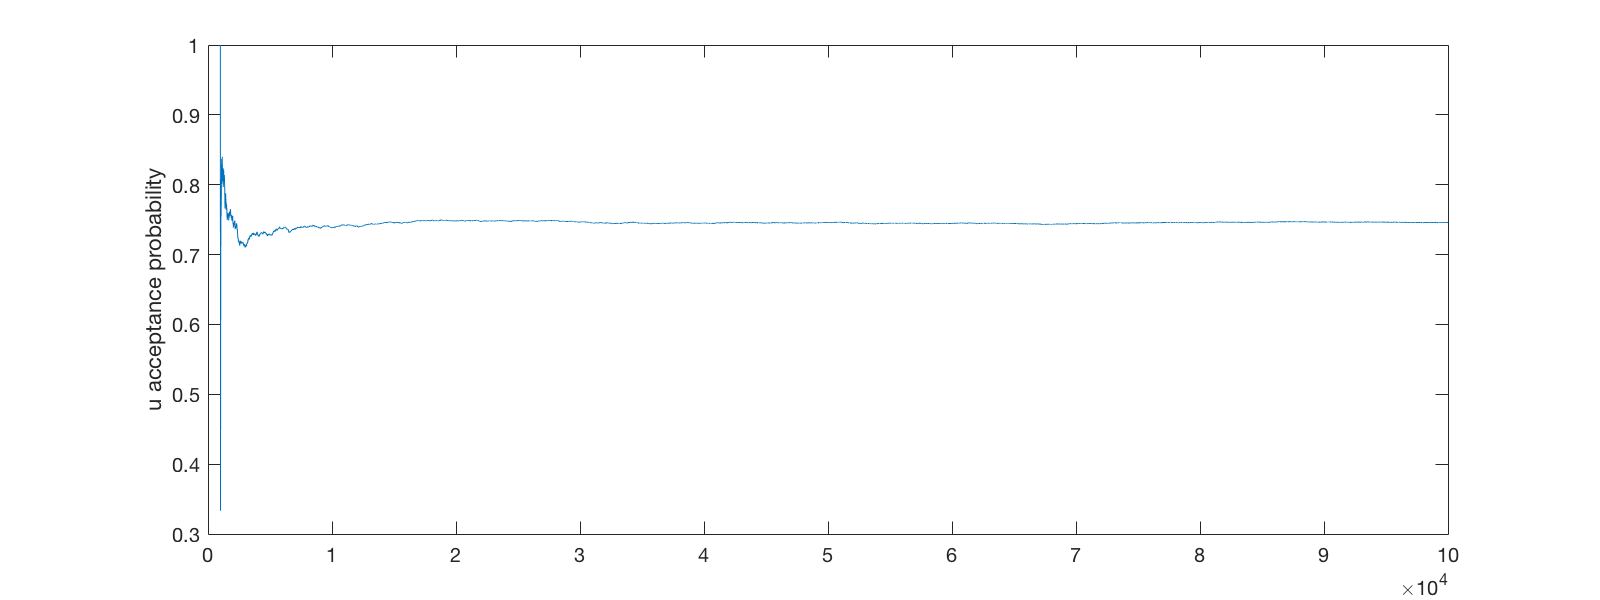
\includegraphics[width=\linewidth]{voting/centered/acceptance_u_probability.png}
    \end{minipage}
    \end{figure}

    \begin{figure}[!htb]
    \begin{minipage}{0.48\textwidth}
        \caption{\label{fig:centered_voting_tau} \cref{alg:hierarchical_tau_alpha} trace of $\tau$}
        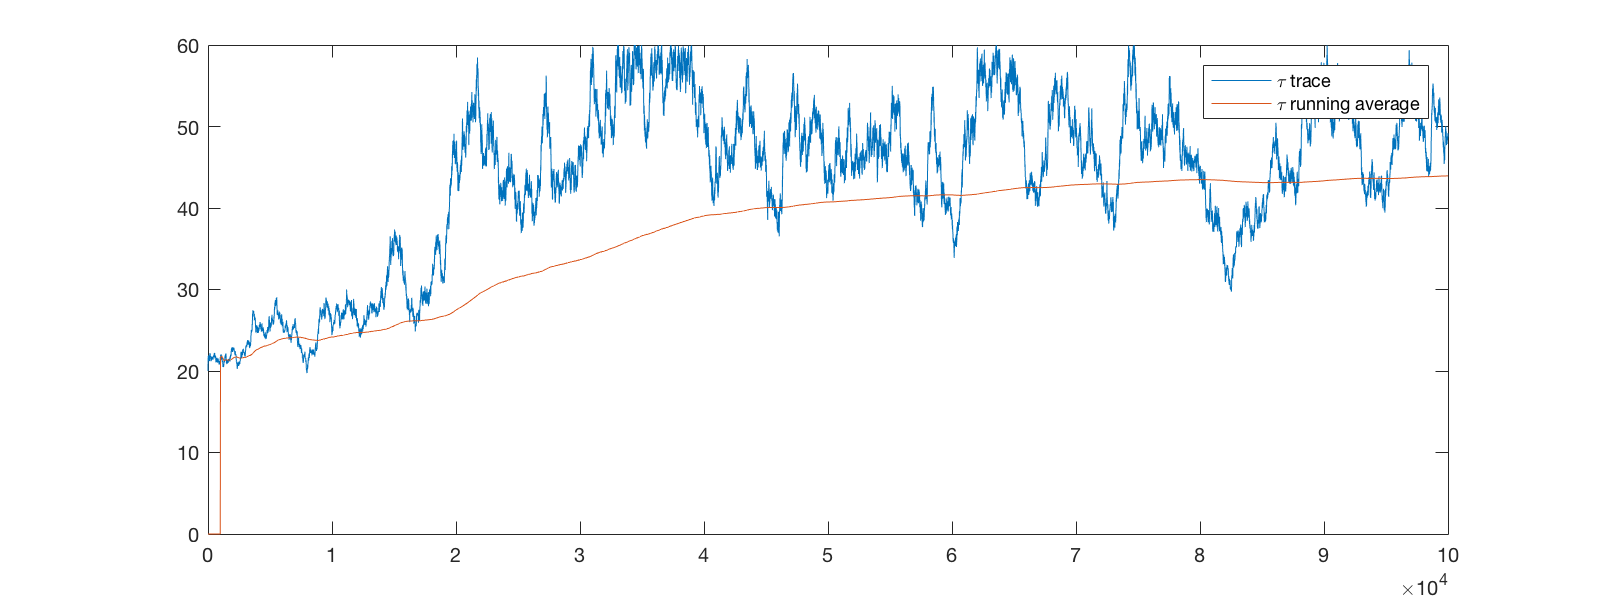
\includegraphics[width=\linewidth]{voting/centered/trace_tau.png}
    \end{minipage}\hfill
    \begin{minipage}{0.48\textwidth}
        \caption{\label{fig:centered_voting_alpha} \cref{alg:hierarchical_tau_alpha} trace of $\alpha$}
        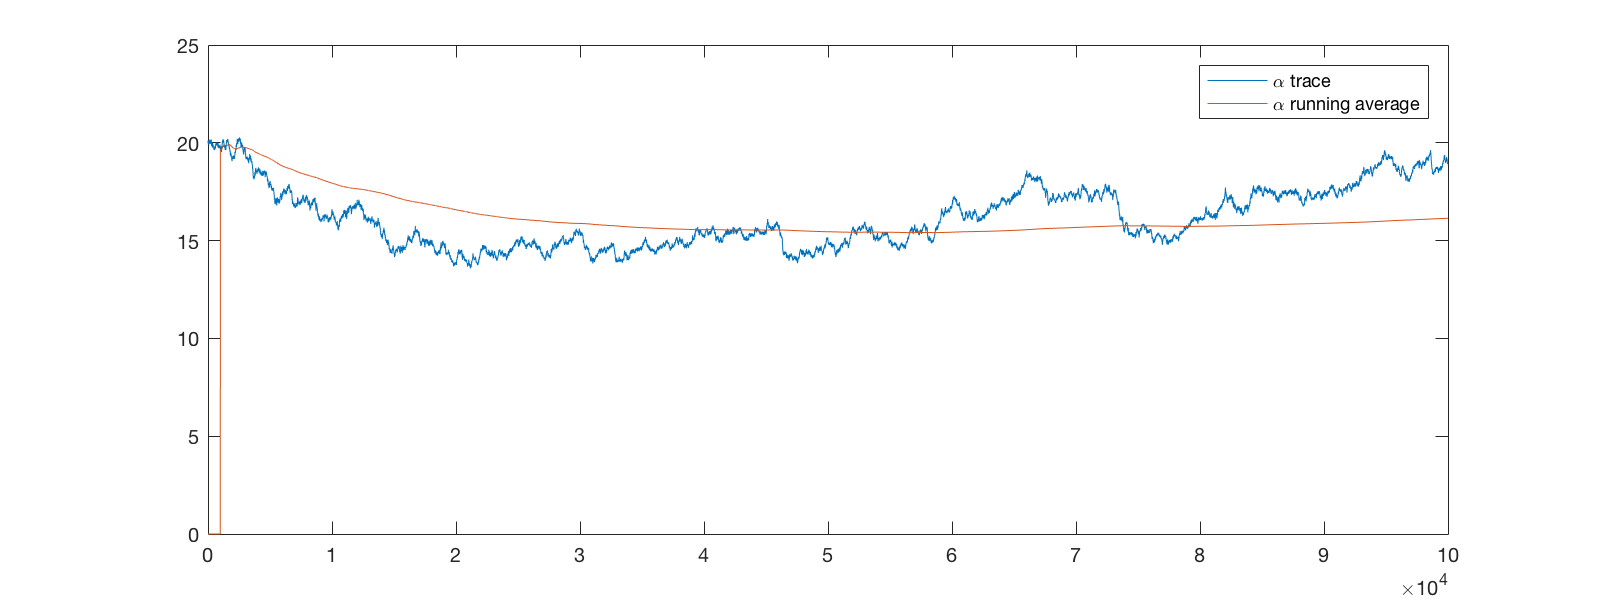
\includegraphics[width=\linewidth]{voting/centered/trace_alpha.png}
    \end{minipage}

    \end{figure}

    Finally, the non-centered \cref{alg:xi_tau_alpha} seems to converge faster than \cref{alg:hierarchical_tau_alpha}, and truncation of the eigenvectors is not necessary. Fixing $\gamma = 0.0001, \beta = 0.1, \tau^{(0)}=20,\alpha^{(0)}=20,\tau\in[0.1,60],\alpha\in[0.1,60],\epsilon_\tau=1,\epsilon_\alpha=1$ and running $100000$ iterations with a burn-in period of $1000$, the accuracy is about 87\%.  See \cref{fig:noncentered_voting_avg}, \cref{fig:noncentered_voting_accept}, \cref{fig:noncentered_voting_tau}, \cref{fig:noncentered_voting_alpha}.

    \begin{figure}[!htb]
    \begin{minipage}{0.48\textwidth}
        \caption{\label{fig:noncentered_voting_avg}\cref{alg:xi_tau_alpha} final average}
        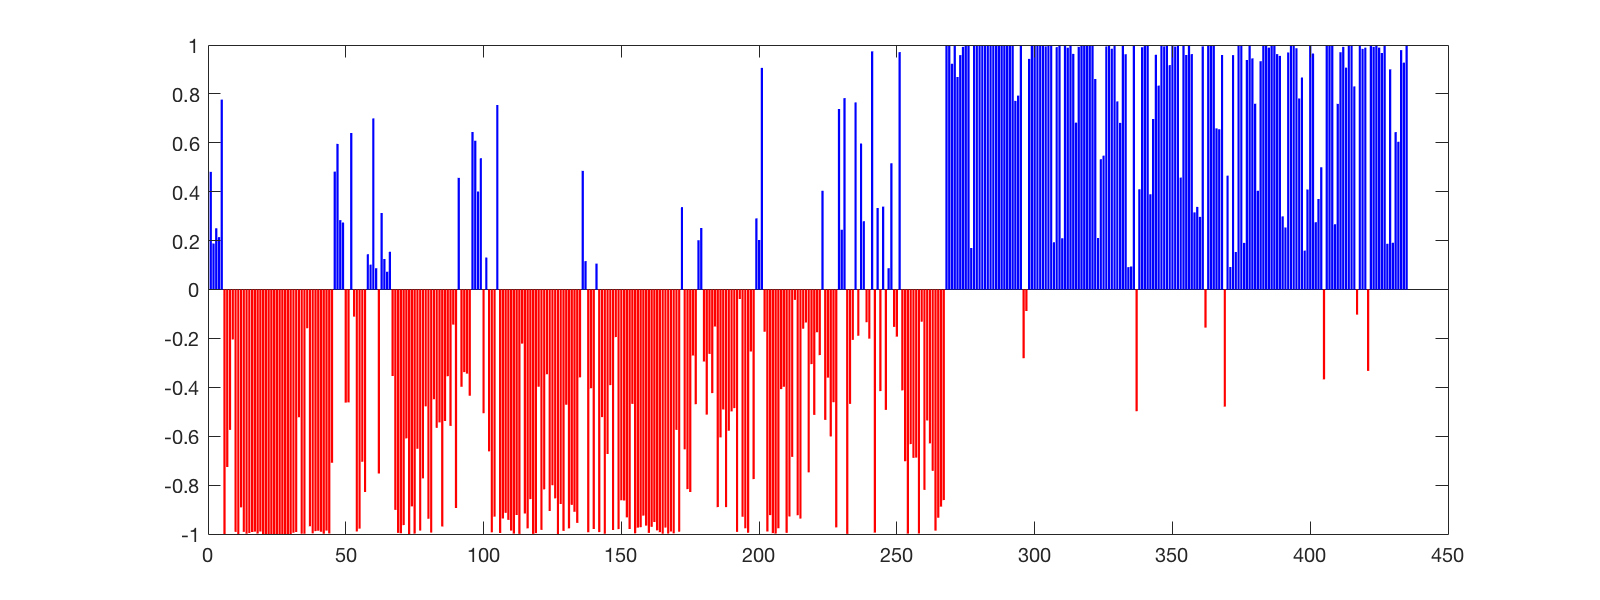
\includegraphics[width=\linewidth]{voting/noncentered/final_avg.png}
    \end{minipage}\hfill
    \begin{minipage}{0.48\textwidth}
        \caption{\label{fig:noncentered_voting_accept} \cref{alg:xi_tau_alpha} average $\xi$ acceptance probablity}
        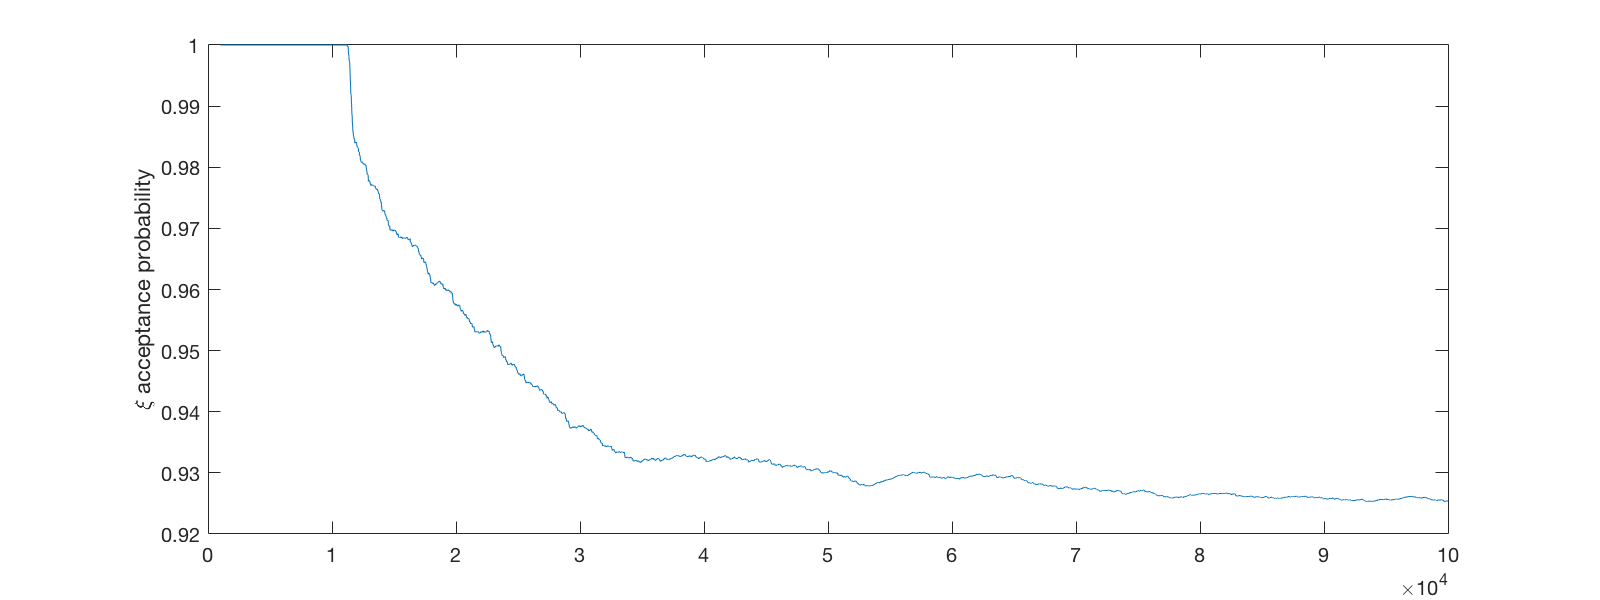
\includegraphics[width=\linewidth]{voting/noncentered/acceptance_xi_probability.png}
    \end{minipage}
    \end{figure}

    \begin{figure}[!htb]
    \begin{minipage}{0.48\textwidth}
        \caption{\label{fig:noncentered_voting_tau}\cref{alg:xi_tau_alpha} trace of $\tau$}
        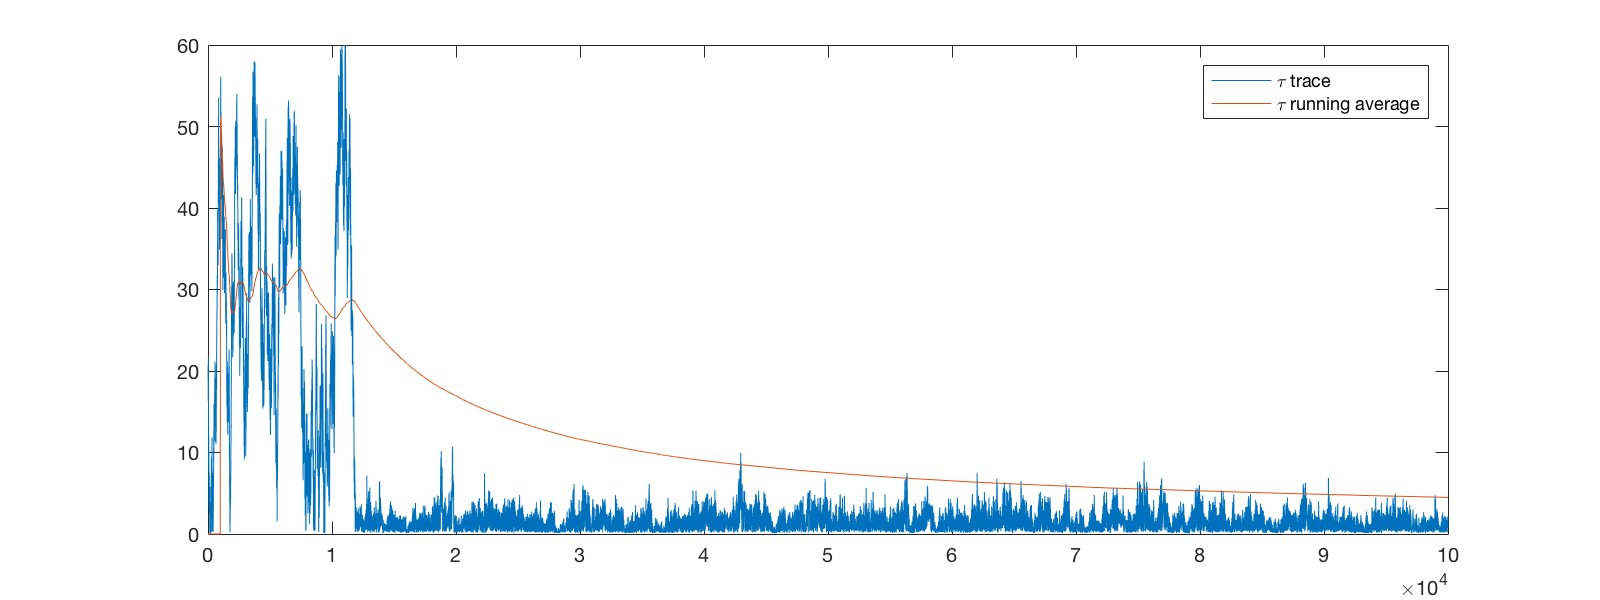
\includegraphics[width=\linewidth]{voting/noncentered/trace_tau.png}
    \end{minipage}\hfill
    \begin{minipage}{0.48\textwidth}
        \caption{\label{fig:noncentered_voting_alpha} \cref{alg:xi_tau_alpha} trace of $\alpha$}
        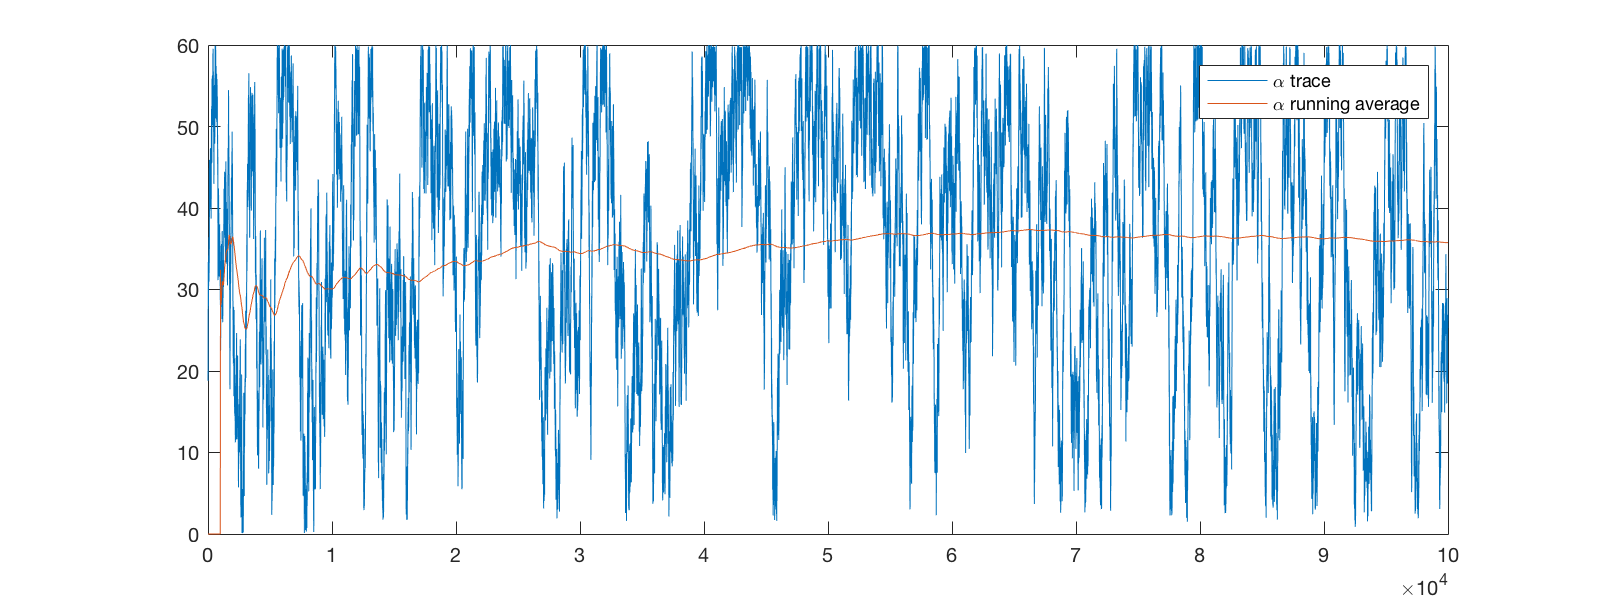
\includegraphics[width=\linewidth]{voting/noncentered/trace_alpha.png}
    \end{minipage}
    \end{figure}

\section{Two moons experiments with models (A) and (B)}
    Using these algorithms, I also ran experiments to cluster the two-moons data set, with $r=1, N = 1000, d = 100, \sigma = 0.1$. We used the self-tuning Laplacian introduced in \cite{SelfTuning}.

    For each of the following experiments, we labeled the same $42$ nodes, $21$ in each half-moon, approximately uniformly spaced. Running \cref{alg:generalpCN} on this data set using only the first 50 eigenvectors with $\gamma=0.0001,\beta=0.4,\tau=1,\alpha=1$ with 100000 iterations and a burn-in period of 1000, we could get around 90\% accuracy.
    \begin{figure}[!htb]
        \begin{minipage}{0.48\textwidth}
            \centering
            \caption{\label{fig:moon_mcmc_gamma_avg} \cref{alg:generalpCN} final average}
            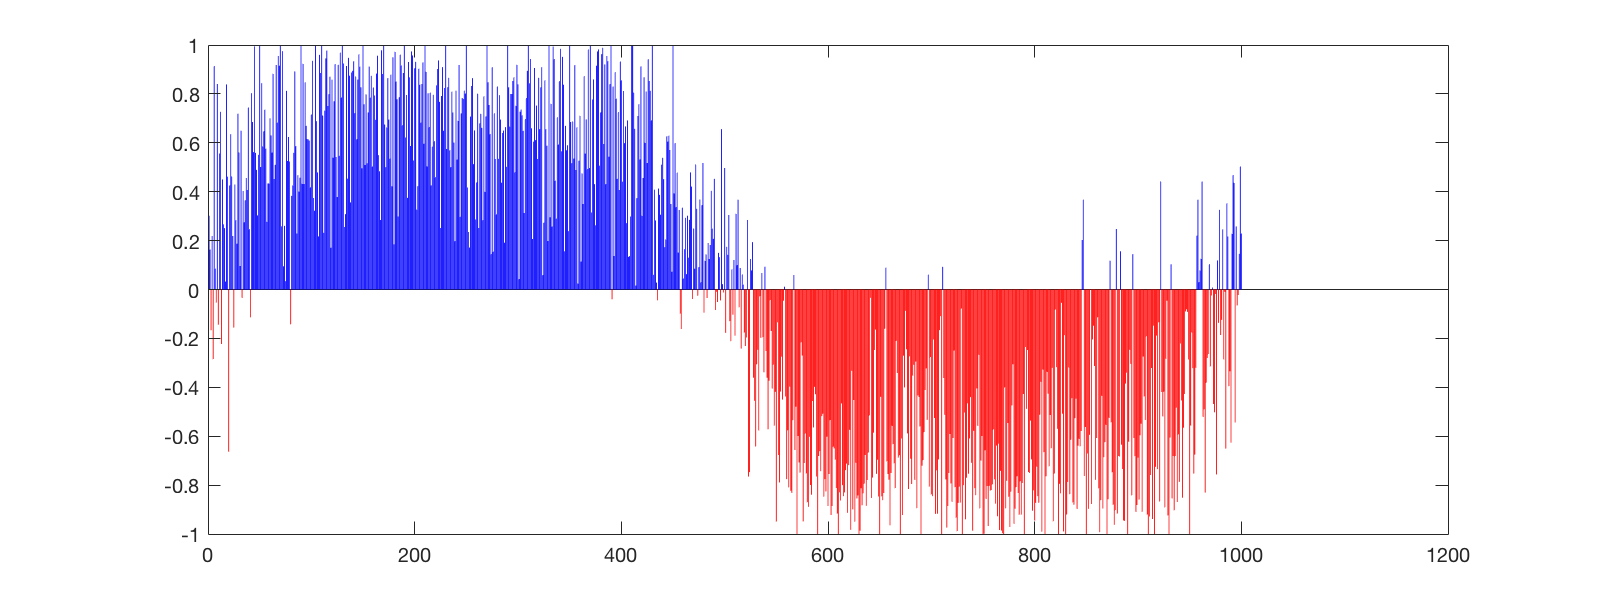
\includegraphics[width=\linewidth]{graphics/moons/mcmc_gamma/u_avg.png}
        \end{minipage} \hfill
        \begin{minipage}{0.48\textwidth}
            \centering
            \caption{\label{fig:moon_mcmc_gamma_accept} \cref{alg:generalpCN} average $u$ acceptance probability}
            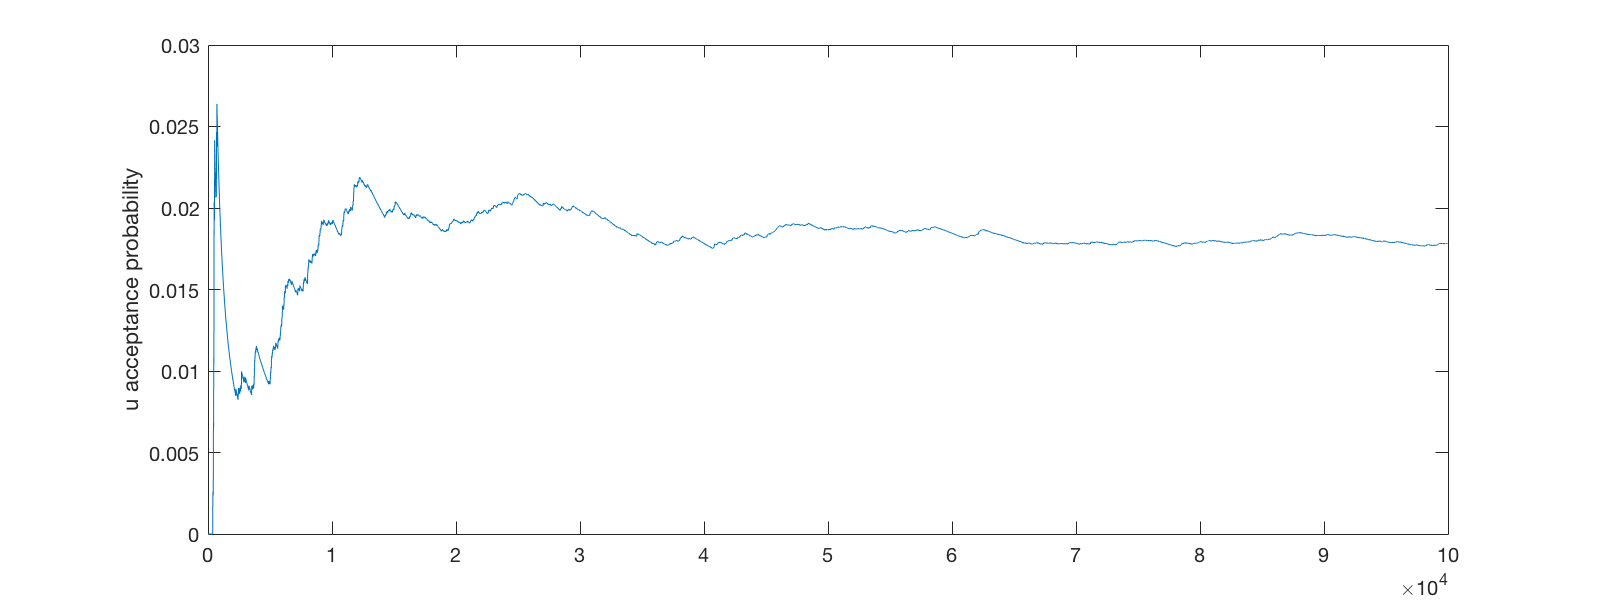
\includegraphics[width=\linewidth]{graphics/moons/mcmc_gamma/u_accept.png}
        \end{minipage}
    \end{figure}

    We now compare the results from the centered (\cref{alg:hierarchical_tau_alpha}) and non-centered (\cref{alg:xi_tau_alpha}) algorithms, truncating the number of eigenvectors to $50$ in both cases. For both algorithms, we fixed $\gamma = 0.1, \beta = 0.4, \tau^{(0)}=20,\alpha^{(0)}=20,\tau\in[0.01,60],\alpha\in[1,60],\epsilon_\tau=0.5,\epsilon_\alpha=1$ and ran $100000$ iterations with a burn-in period of $1000$. With these settings, \cref{alg:hierarchical_tau_alpha} achieves around 90\% accuracy, while \cref{alg:xi_tau_alpha} achieves around 98\%. It still appears that the non-centered algorithm converges faster than the centered algorithm. If the centered algorithm is initialized at $\tau^{(0)} = 1$, the final classification accuracy is very similar to that of the non-centered algorithm. See \cref{fig:moon_centered_avg}, \cref{fig:moon_centered_accept}, \cref{fig:moon_centered_tau}, \cref{fig:moon_centered_alpha}, \cref{fig:moon_noncentered_avg}, \cref{fig:moon_noncentered_accept}, \cref{fig:moon_noncentered_tau}, \cref{fig:moon_noncentered_alpha}.

    \begin{figure}[!htb]
        \begin{minipage}{0.48\textwidth}
            \centering
            \caption{\label{fig:moon_centered_avg} \cref{alg:hierarchical_tau_alpha} final average}
            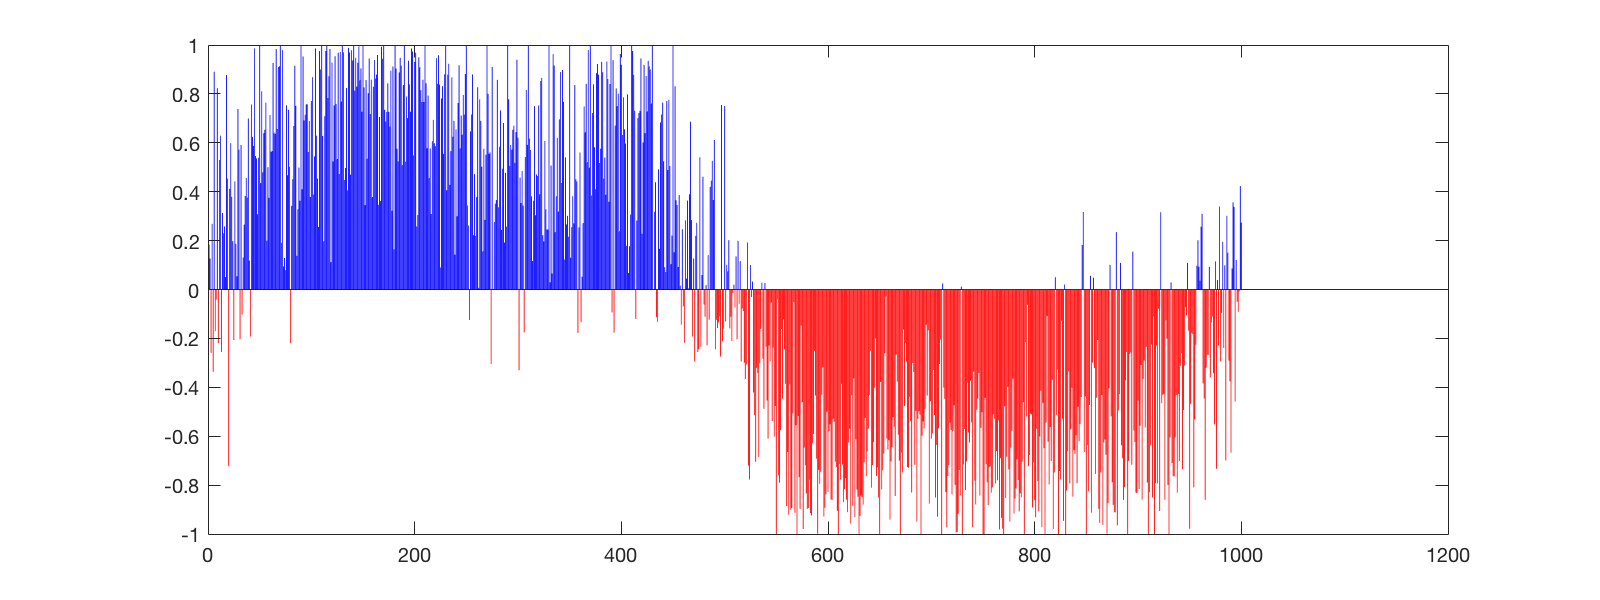
\includegraphics[width=\linewidth]{graphics/moons/centered/final_avg.png}
        \end{minipage} \hfill
        \begin{minipage}{0.48\textwidth}
            \centering
            \caption{\label{fig:moon_centered_accept} \cref{alg:hierarchical_tau_alpha} average $u$ acceptance probability}
            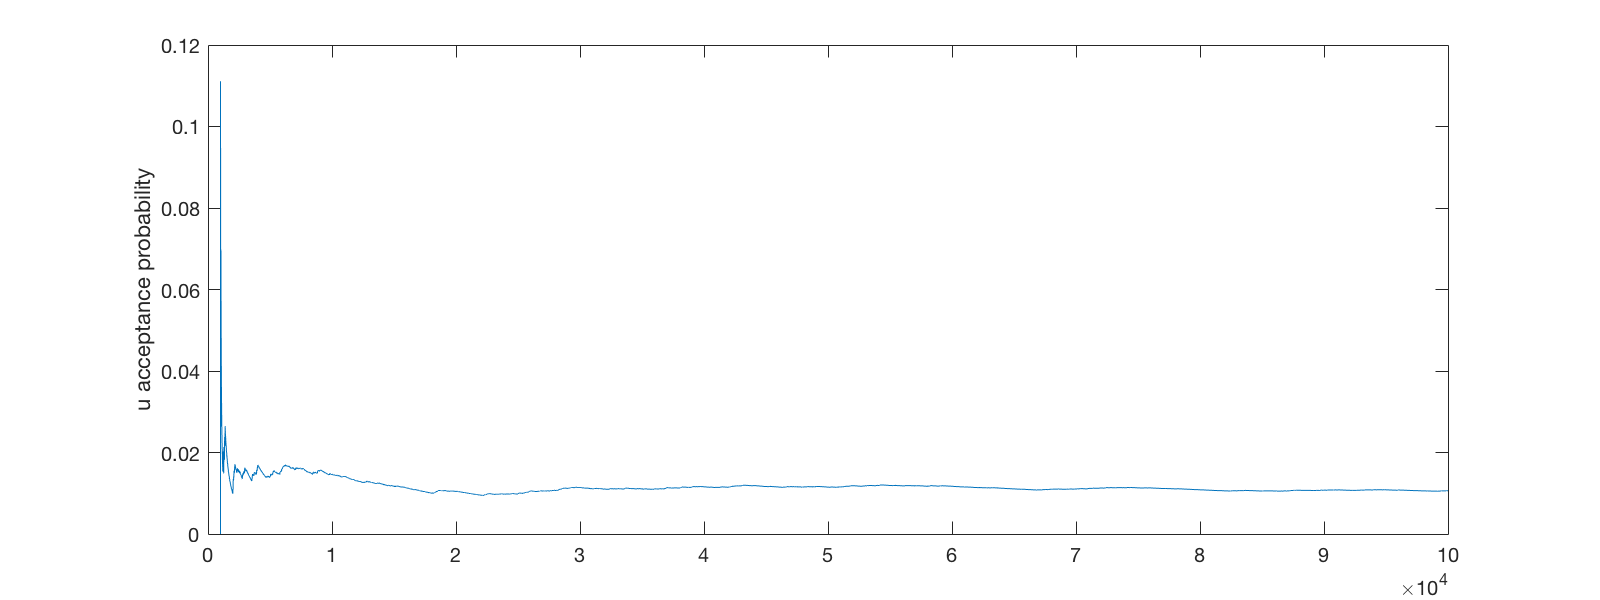
\includegraphics[width=\linewidth]{graphics/moons/centered/acceptance_u_probability.png}
        \end{minipage}
    \end{figure}

    \begin{figure}[!htb]
        \begin{minipage}{0.48\textwidth}
            \centering
            \caption{\label{fig:moon_centered_tau} \cref{alg:hierarchical_tau_alpha}, trace $\tau$}
            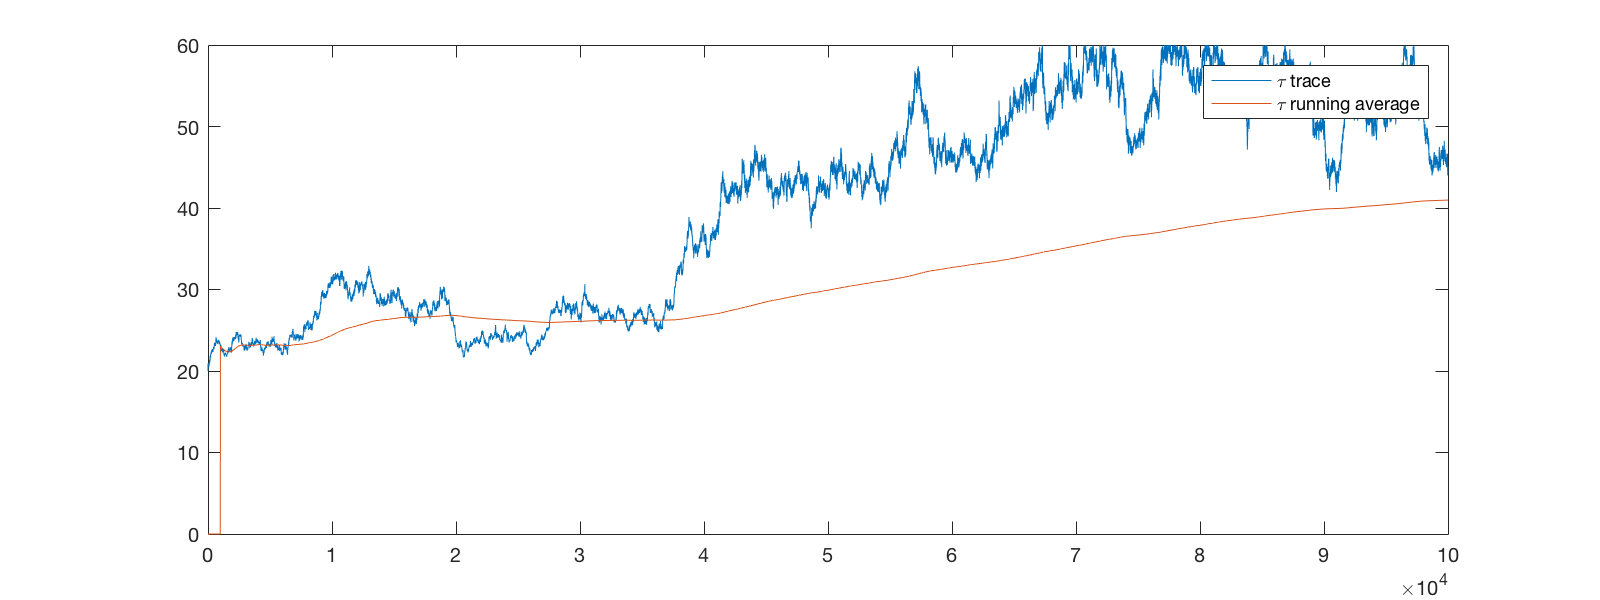
\includegraphics[width=\linewidth]{graphics/moons/centered/trace_tau.png}
        \end{minipage} \hfill
        \begin{minipage}{0.48\textwidth}
            \centering
            \caption{\label{fig:moon_centered_alpha} \cref{alg:hierarchical_tau_alpha}, trace $\alpha$}
            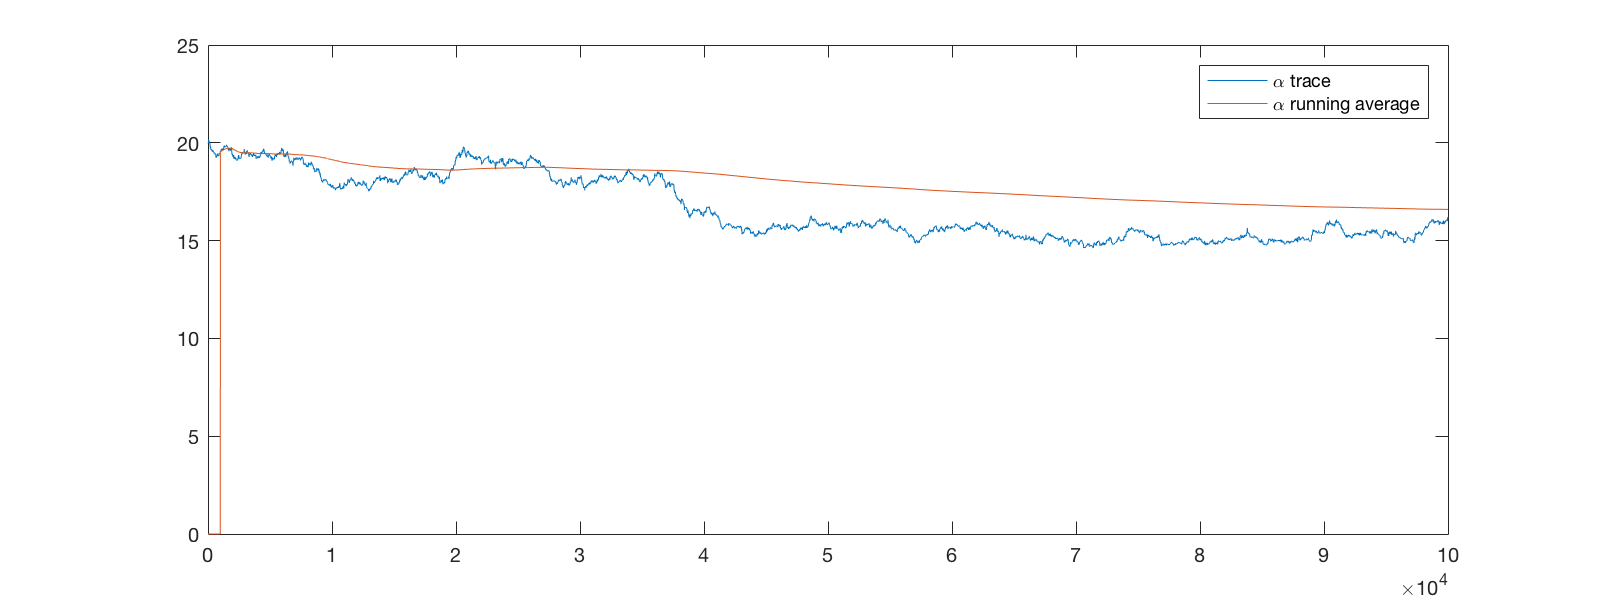
\includegraphics[width=\linewidth]{graphics/moons/centered/trace_alpha.png}
        \end{minipage}
    \end{figure}

    \begin{figure}[!htb]
        \begin{minipage}{0.48\textwidth}
            \centering
            \caption{\label{fig:moon_noncentered_avg} \cref{alg:xi_tau_alpha} final average}
            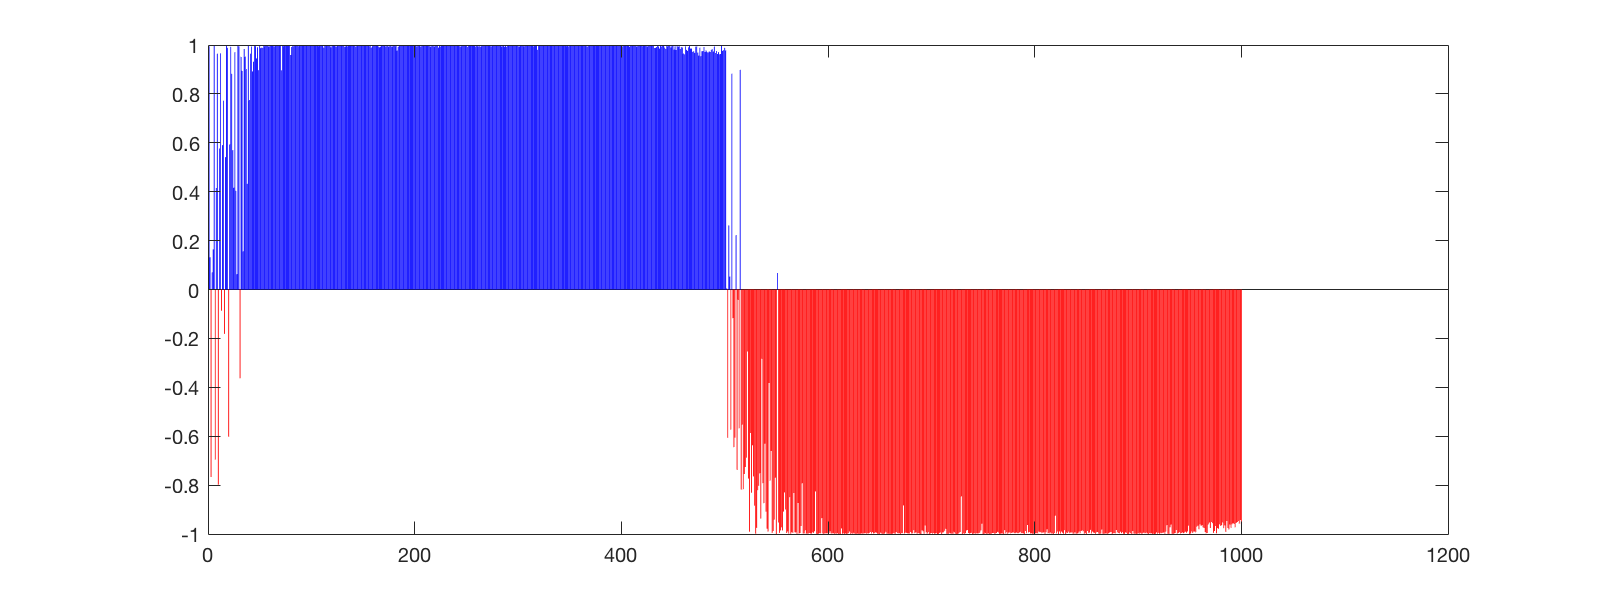
\includegraphics[width=\linewidth]{graphics/moons/noncentered/final_avg.png}
        \end{minipage} \hfill
        \begin{minipage}{0.48\textwidth}
            \centering
            \caption{\label{fig:moon_noncentered_accept} \cref{alg:xi_tau_alpha} average $\xi$ acceptance probability}
            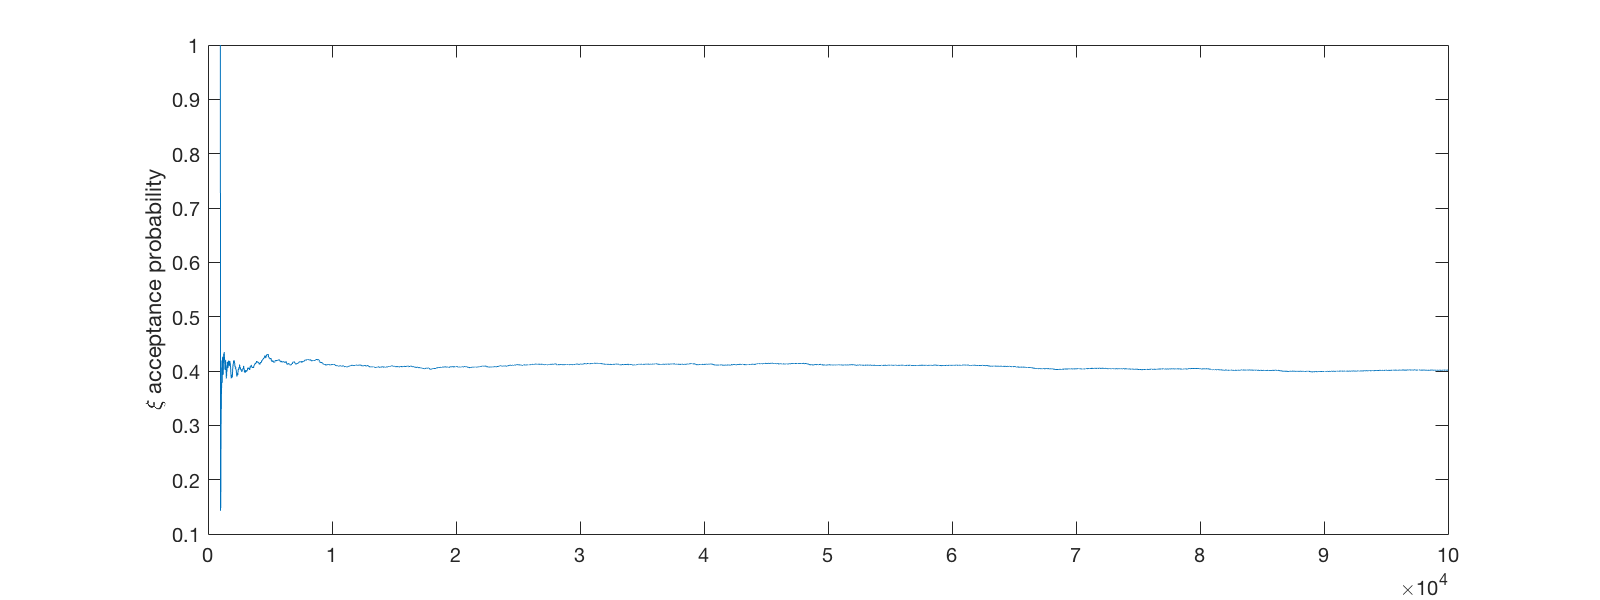
\includegraphics[width=\linewidth]{graphics/moons/noncentered/acceptance_xi_probability.png}
        \end{minipage}
    \end{figure}

    \begin{figure}[!htb]
        \begin{minipage}{0.48\textwidth}
            \centering
            \caption{\label{fig:moon_noncentered_tau} \cref{alg:xi_tau_alpha}, trace $\tau$}
            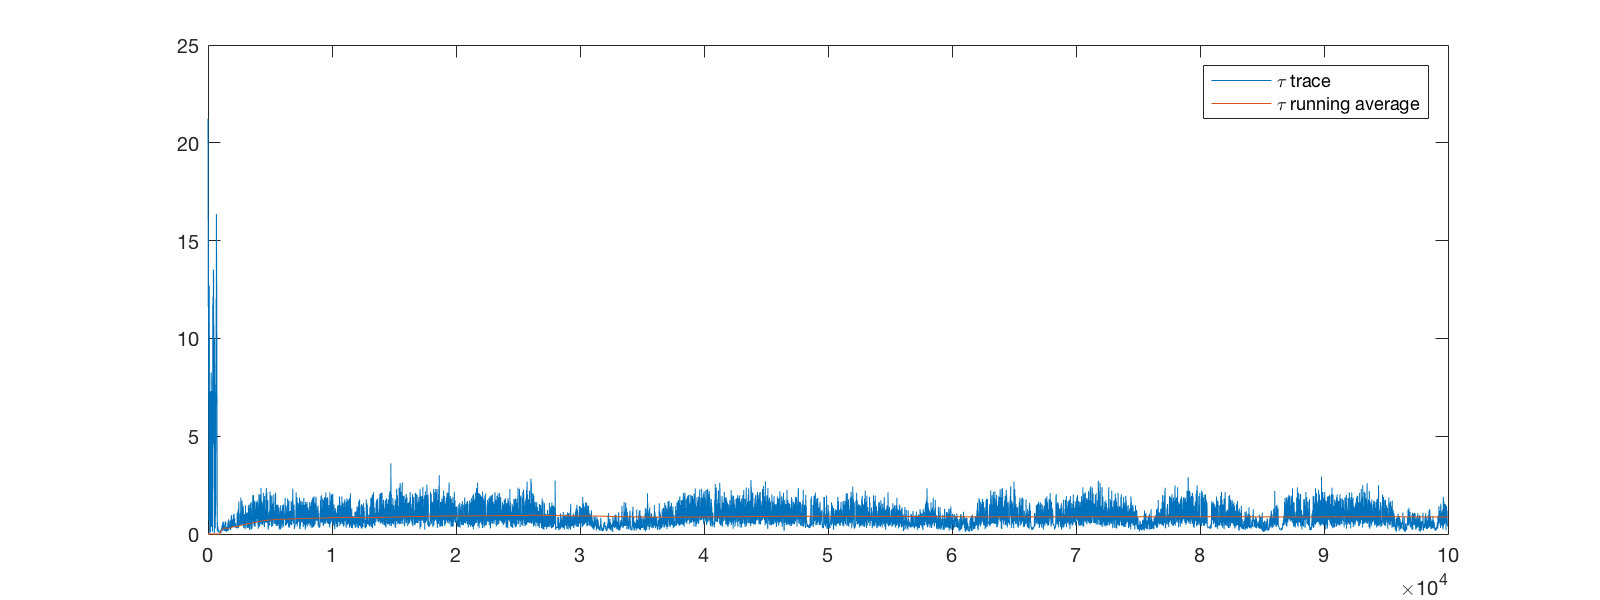
\includegraphics[width=\linewidth]{graphics/moons/noncentered/trace_tau.png}
        \end{minipage} \hfill
        \begin{minipage}{0.48\textwidth}
            \centering
            \caption{\label{fig:moon_noncentered_alpha} \cref{alg:xi_tau_alpha}, trace $\alpha$}
            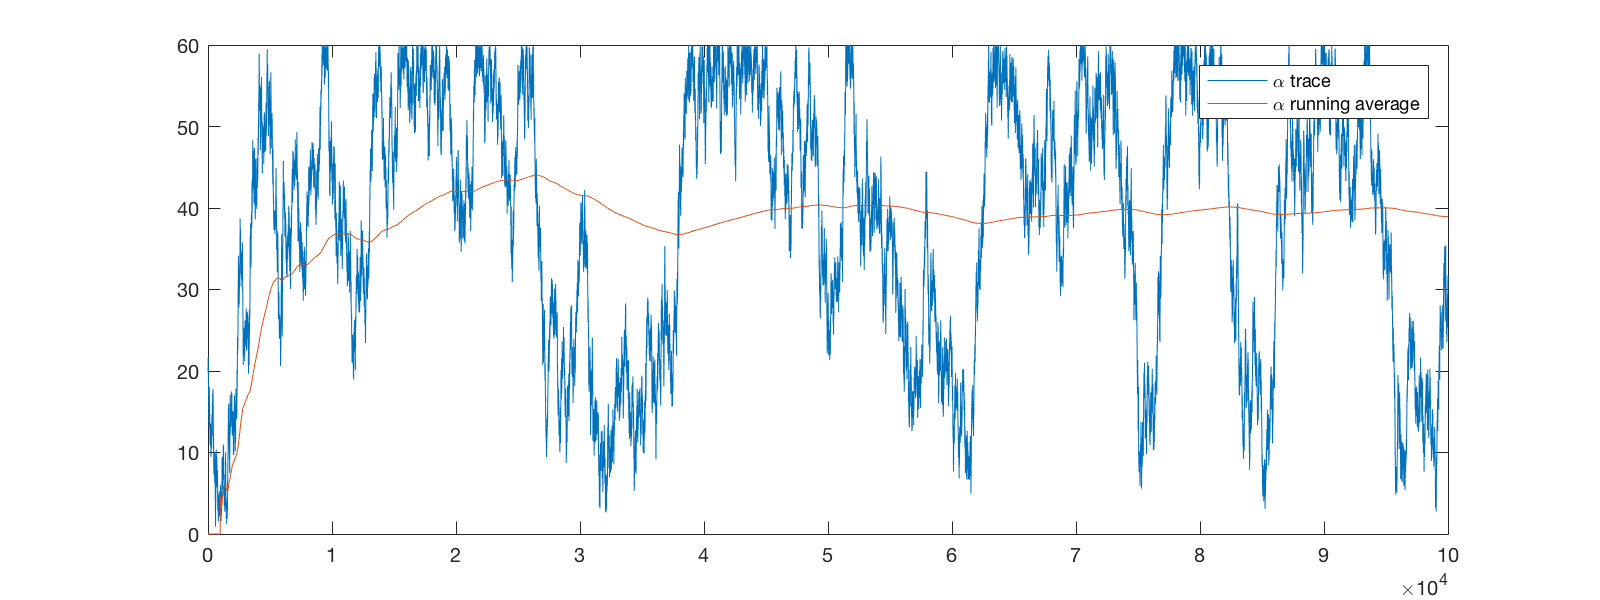
\includegraphics[width=\linewidth]{graphics/moons/noncentered/trace_alpha.png}
        \end{minipage}
    \end{figure}

    Notice the convergence of $\tau$ and its low variance in the samples for the non-centered self-tuning algorithm.

\fi

\section{Experiments comparing hierarchical and nonhierarchical algorithms}
    Inspired by the experiment comparing the different clustering algorithms given in \cite{BeLuStZy17}, we ran a similar set of experiments to determine if a hierarchical approach was beneficial to clustering. The clustering algorithms we want to compare are: Fiedler thresholding, nonhierarchical pCN, and two hierarchical algorithms for learning $\tau,\alpha$ as well as the classifying function $u$.
    For each of the four algorithms tested, 50 random realizations of the two moons data set were generated with $r=1,N=2000,d=100,$ and varying $\sigma$. We used the same RNG seed for the trials across different algorithms so that these 50 realizations are consistent over the different algorithms tested. With each two moons realization, we tested the classification accuracy with varying fidelity percents for the labeled data. Again, the chosen labeled set $Z'$ is consistent across the trials for different algorithms. Our results are summarized in \cref{fig:compare_hier}.

    \begin{figure}[!htb]
    \label{fig:compare_hier}
    \caption{Classification accuracy of different algorithms for two moons dataset compared with $\sigma$ and percent fidelity. Plotted is the median classification accuracy with error bars that indicate the 25 and 75-th quantiles over the 50 trials for each parameter combination. For the pCN and hierarchical algorithms, we used spectral projection up to the first 50 eigenvectors. We ran 100000 iterations with a burn-in period of 1000, and we fixed $\gamma = 0.1$.}
    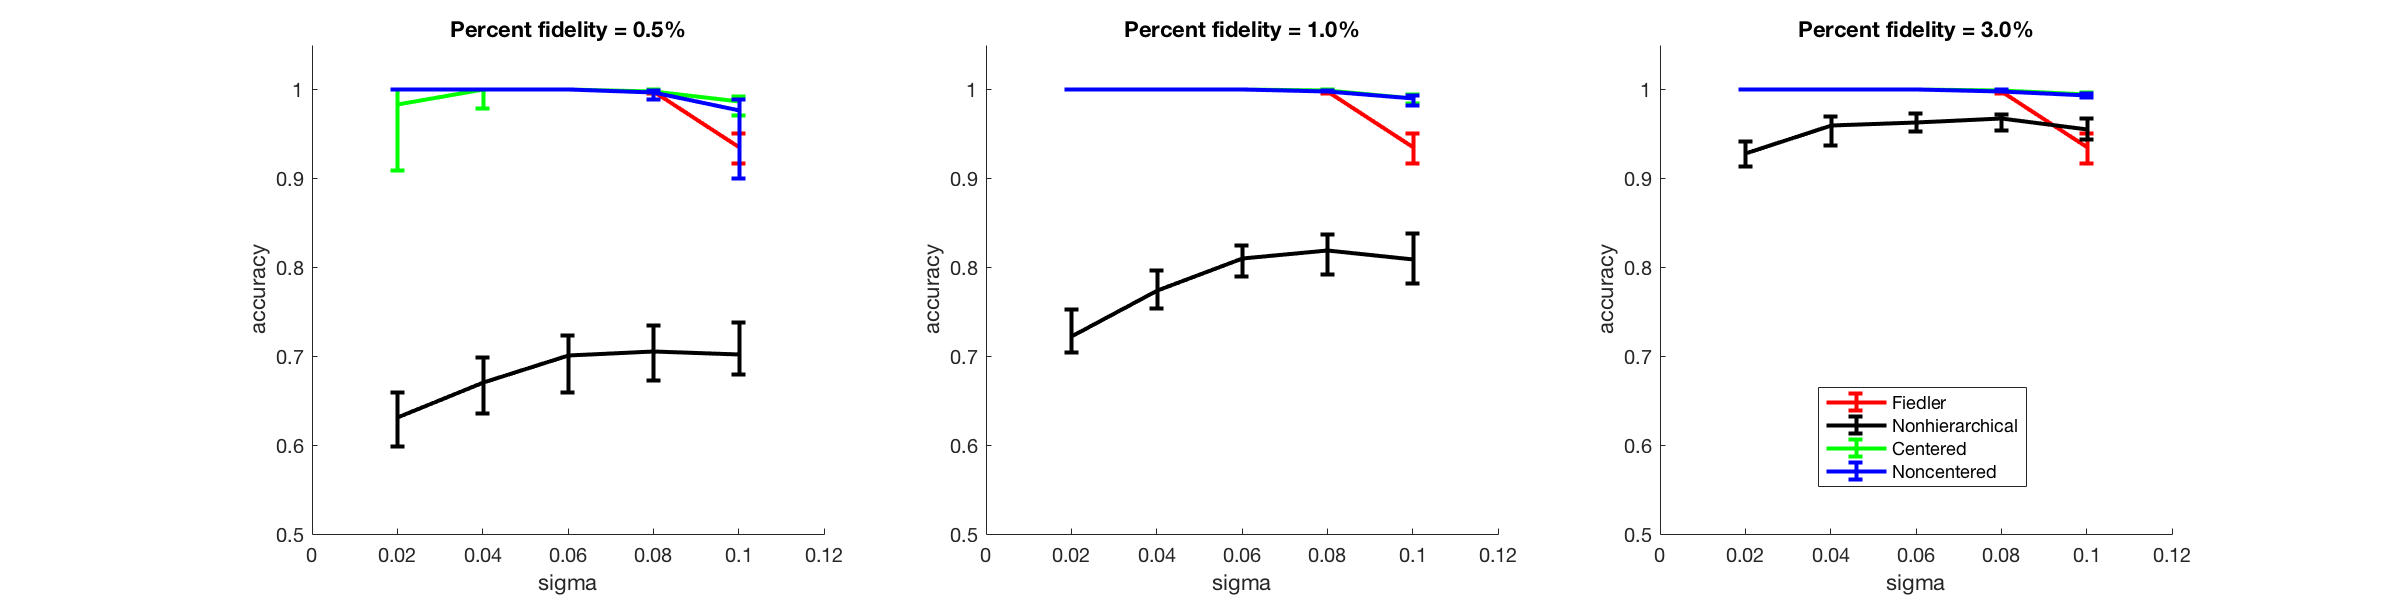
\includegraphics[width=\linewidth]{compare/summary.png}
    \end{figure}

    \subsection{Learning $\tau$ and $\alpha$}
        In these experiments, the hierarchical algorithms performed much better in classifying the two moons dataset than the nonhierarchical algorithm. We fixed $\tau=\alpha=1$ in the nonhierarchical pCN, while we set $\tau^{(0)}=\alpha^{(0)} = 1$ for the hierarchical algorithms. In the hierarchical algorithms, we allowed $\tau \in [0.01,60]$ and $\alpha \in [0.1,60]$ as the uniform priors. The medians of the average values of $\alpha$ given by the hierarchical algorithms are shown in \cref{fig:compare_alpha}.
        \begin{figure}[!htb]
        \label{fig:compare_alpha}
        \caption{Average values of $\alpha$ from the MCMC. Plotted is the median of the averages of $\alpha$ with error bars that indicate the 25 and 75-th quantiles over the 50 trials for each parameter combination. Notice that $\alpha$ is on average much larger in the hierarchical algorithms.}
        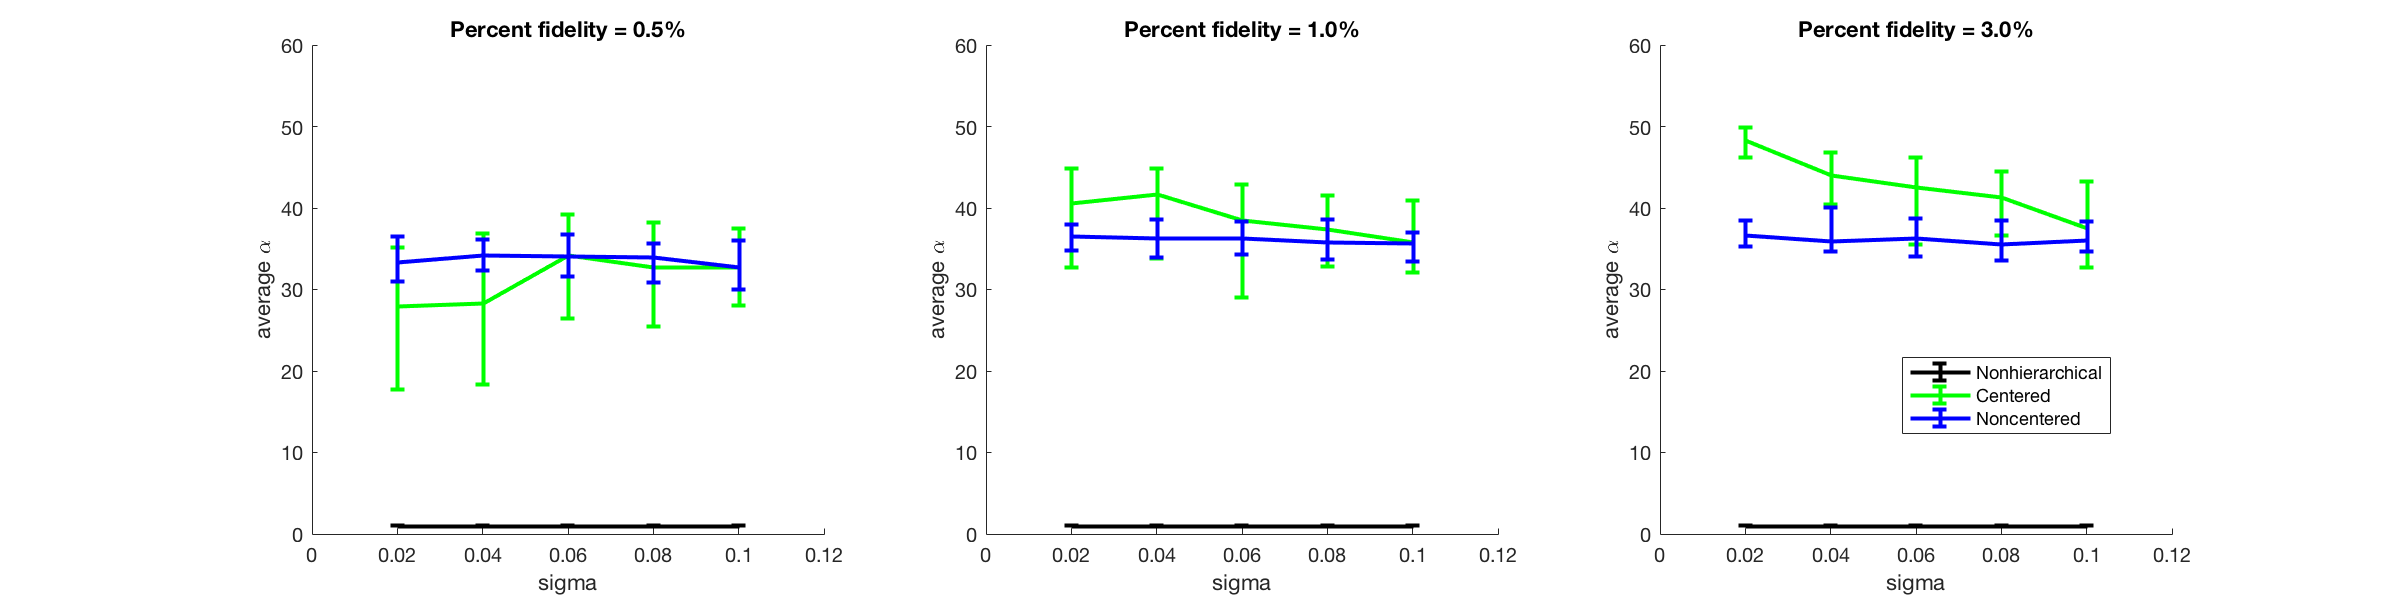
\includegraphics[width=\linewidth]{compare/alpha_averages.png}
        \end{figure}

        It appears that fixing $\alpha = 1$ in the nonhierarchical algorithm is partially responsible for the discrepancy in performance. With small $\alpha$, the prior on $u$ drops off more slowly with the higher eigenvectors, while larger $\alpha$ enforces that these higher eigenvectors have less influence on $u$. This suggests that for the two moons data set, information for binary classification is concentrated in the lower eigenvectors, as expected.

\section{Experiments with model (C)}
    \subsection{$M$ and $\sigma$ relation}
        We tested \cref{alg:hier_t_a_M} on the two moons dataset with varying $\sigma$, fixing $1\%$ labeled nodes. We also fixed $\tau=2,\alpha=35$ by setting $\epsilon_1=\epsilon_2=0$, so the algorithm is only learning $\xi$ and $M$. We initialized $M^{(0)} = 50$, and the uniform prior of $M \sim \mathsf{U}(1, 70)$. We can see that for small $\sigma = 0.06$, $M$ is small as only the first few eigenvectors are necessary (see \cref{fig:learnM_sigma_0.06}). However, when we choose a larger $\sigma = 0.2$, $M$ needs to be larger (see \cref{fig:learnM_sigma_0.20}). For $\sigma = 0.06$, the classification accuracy was 100\%. For $\sigma = 0.2$, the classification accuracy was 91.97\%.

        \begin{figure}[!htb]
        \caption{\label{fig:learnM_sigma_0.06} $\sigma=0.06$, trace of $M$}
        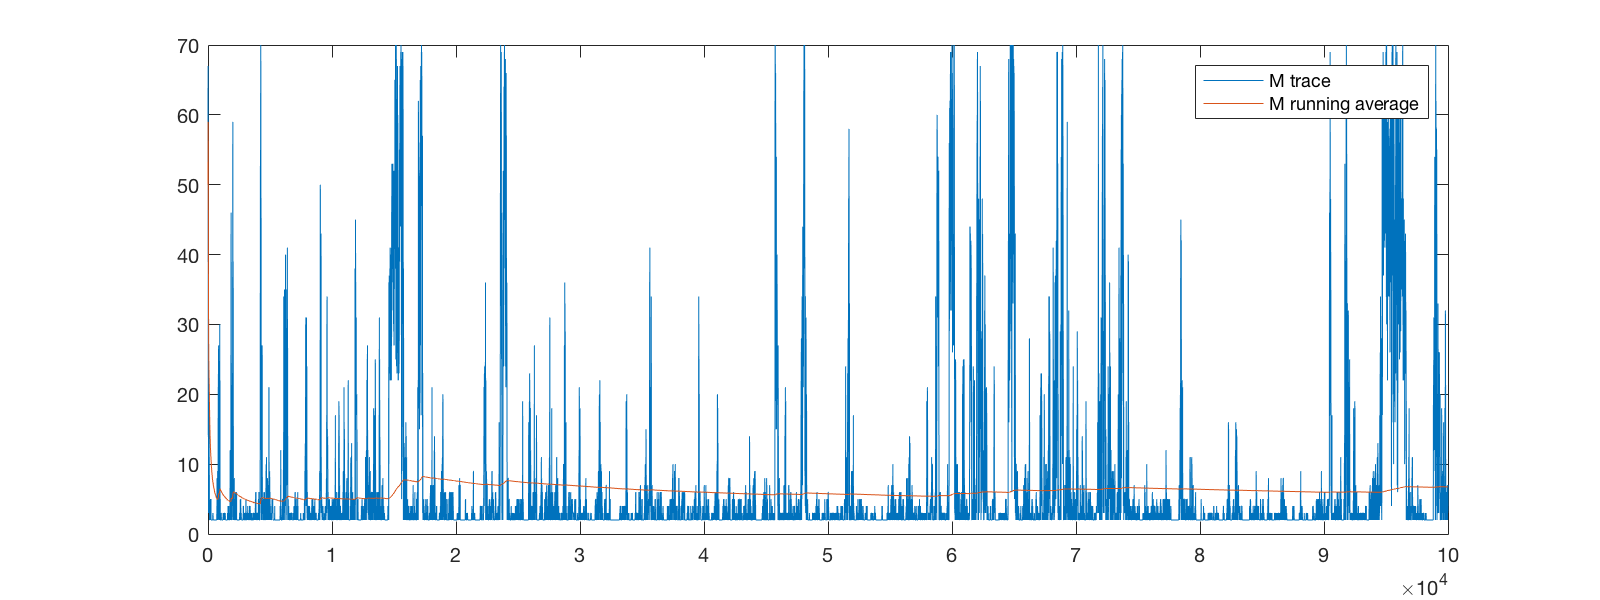
\includegraphics[width=\linewidth]{learnM/moons/hier/sigma_0_06/M_trace.png}
        \end{figure}
        \begin{figure}[!htb]
        \caption{\label{fig:learnM_sigma_0.20} $\sigma=0.2$, trace of $M$}
        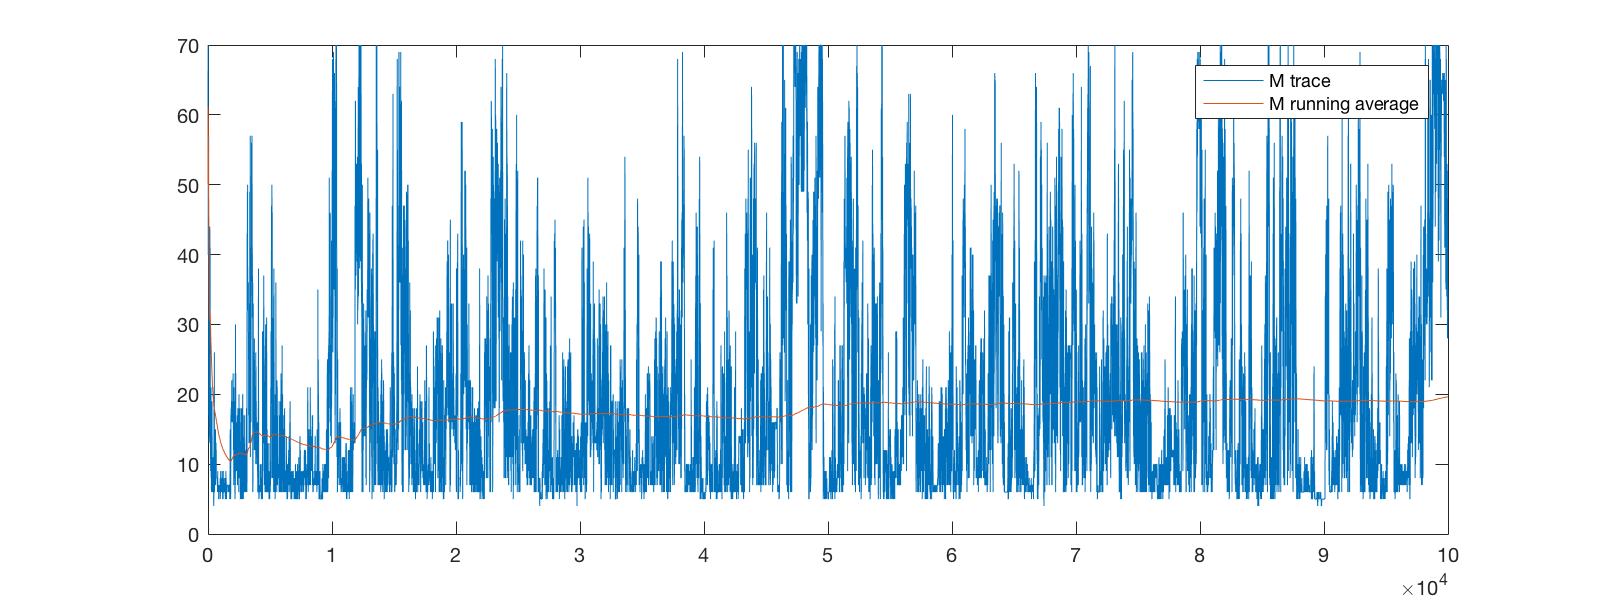
\includegraphics[width=\linewidth]{learnM/moons/hier/sigma_0_20/M_trace.png}
        \end{figure}
    
    \subsection{Nonhierarchical vs. Hierarchical}
        We will compare \cref{alg:generalpCN}, pCN, with fixed $\tau$ and $\alpha$ against \cref{alg:hier_t_a_M} with the same fixed $\tau$ and $\alpha$, but learning $M$.
        \subsubsection{Voting records}
            The nonhierarchical algorithm for learning $\tau$ and $\alpha$ gave expected values of $\tau$ and $\alpha$ as $\tau \approx 2$ and $\alpha \approx 35$, so I chose those parameters for the pCN and for \cref{alg:hier_t_a_M}. For the pCN, all $435$ eigenvectors were used. I narrowed the range of $M$ allowed in \cref{alg:hier_t_a_M} to 1 to 70. 5 labeled nodes were selected, consistent across the two methods. In this particular realization (seeded with $\text{rng}(5)$), the hierarchical algorithm achieves $87.74\%$ while the nonhierarchical algorithm achieves $87.67\%$ classification accuracy. \cref{fig:voting_nonhier_u_avg}, \cref{fig:voting_nonhier_u_accept} , and \cref{fig:voting_nonhier_senator_traces} show the results of the pCN. \cref{fig:voting_hier_M_trace}, \cref{fig:voting_hier_u_avg}, \cref{fig:voting_hier_xi_M_accept} show the results the hierarchical algorithm. Notice in \cref{fig:voting_hier_M_trace} that there seems to be an important eigenvector for classification indexed around 30, as $M$ seldom drops below $30$. Looking at the eigenvectors around index 30, I plotted the 34th eigenvector in \cref{fig:voting_hier_eigenvector}. From a purely visual perspective, it does appear that this eigenvector corresponds decently to the final classification in \cref{fig:voting_hier_u_avg} by looking at where some of the ``spikes'' are. After trying some other realizations, it seems that being hierarchical may have some benefits, but more experiments are needed.

            \begin{figure}[!htb]
            \begin{minipage}{0.48\textwidth}
                \centering
                \caption{\label{fig:voting_nonhier_u_avg} \cref{alg:generalpCN}, average of $S(u)$}
                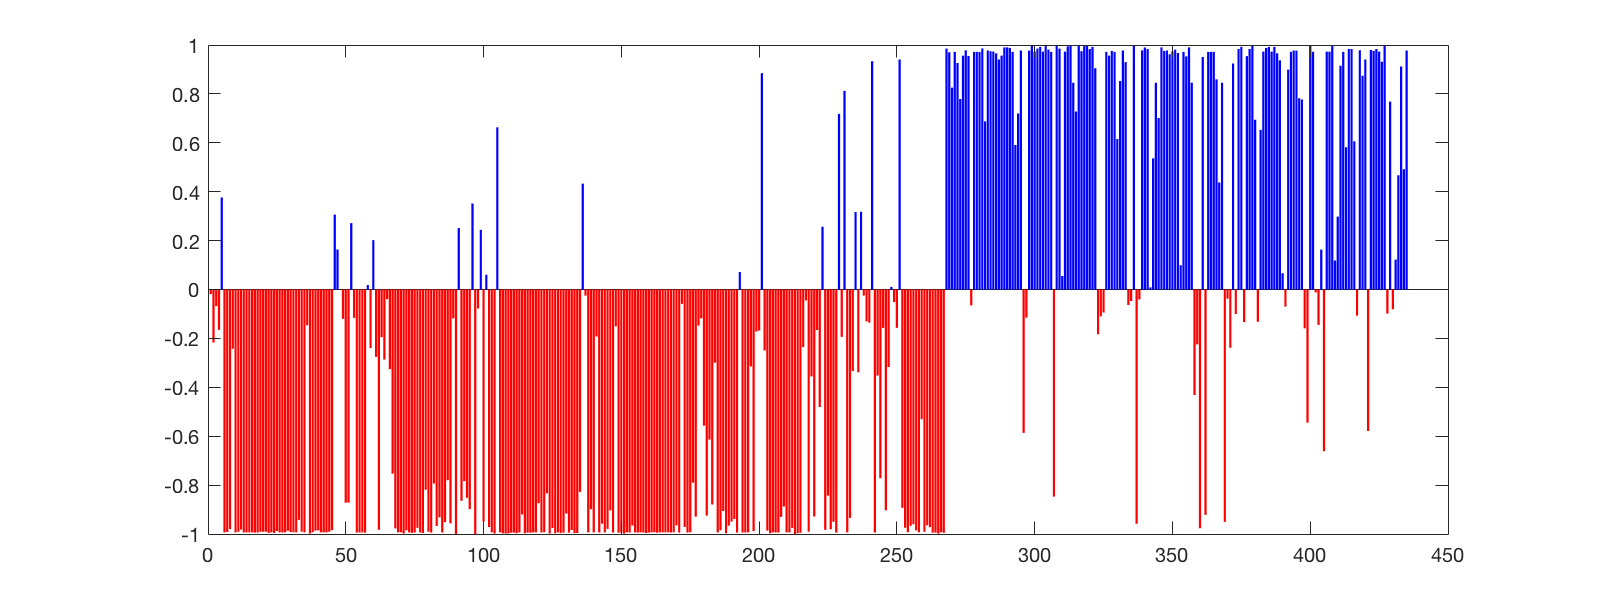
\includegraphics[width=\linewidth]{learnM/voting/nonhier/u_avg.png}
            \end{minipage} \hfill
            \begin{minipage}{0.48\textwidth}
                \centering
                \caption{\label{fig:voting_nonhier_u_accept} \cref{alg:generalpCN}, $u$ acceptance probability}
                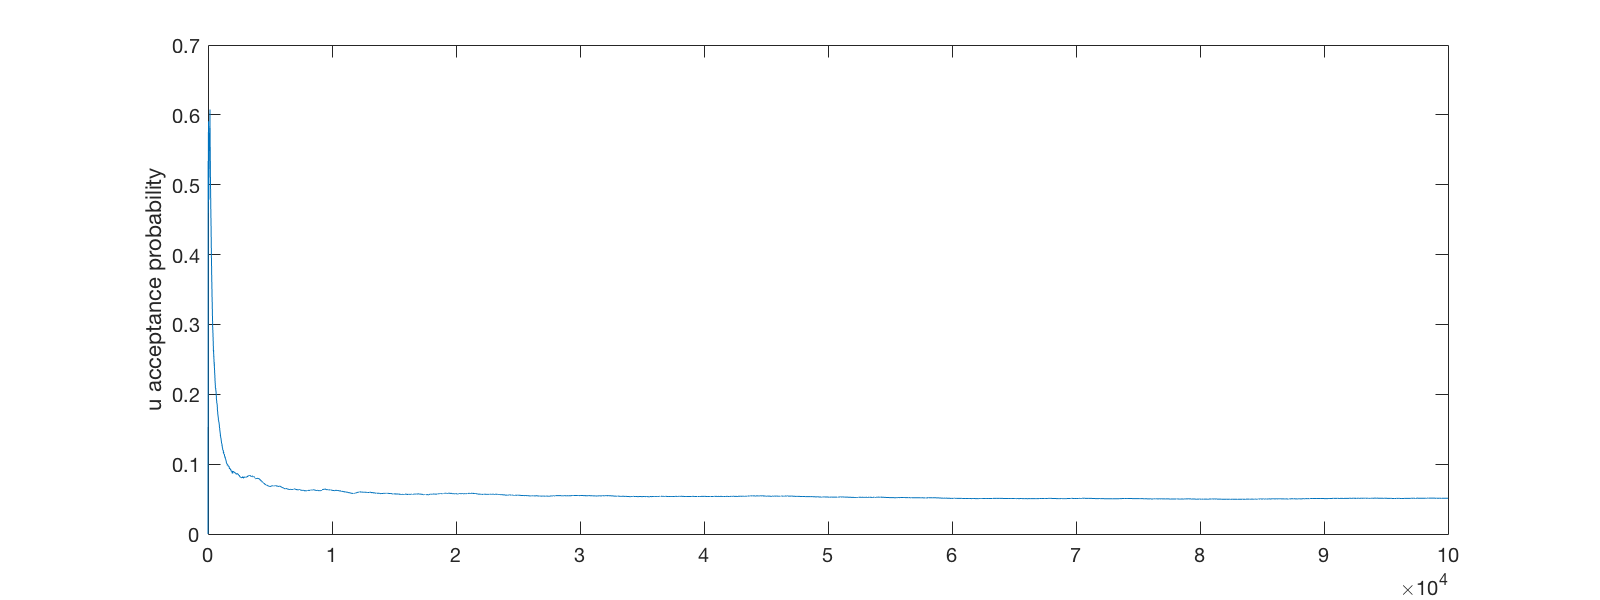
\includegraphics[width=\linewidth]{learnM/voting/nonhier/u_accept.png}
            \end{minipage}
            \end{figure}

            \begin{figure}[!htb]
            \centering
            \caption{\label{fig:voting_nonhier_senator_traces} \cref{alg:generalpCN}, running average of $S(u(i))$ for select $i$}
            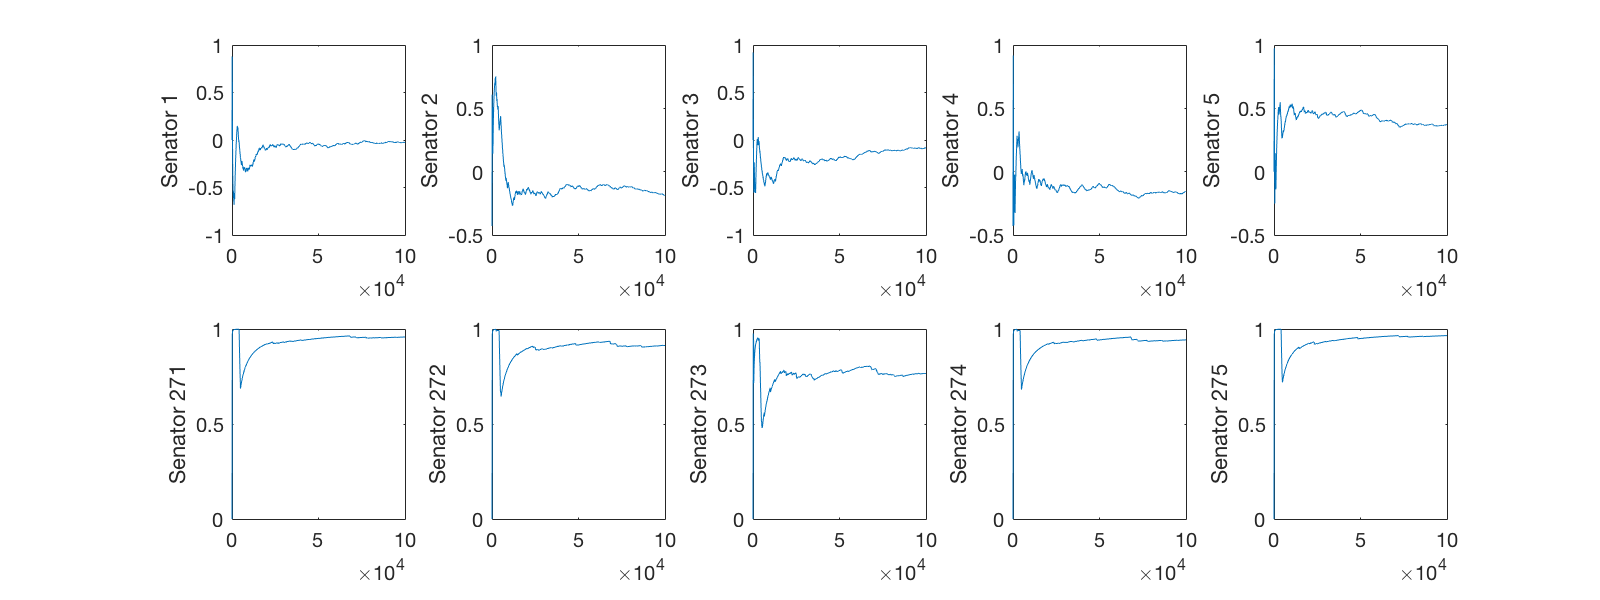
\includegraphics[width=0.8\linewidth]{learnM/voting/nonhier/senator_traces.png}
            \end{figure}

            \begin{figure}[!htb]
            \begin{minipage}{0.48\textwidth}
                \centering
                \caption{\label{fig:voting_hier_u_avg} \cref{alg:hier_t_a_M}, average of $S(u)$}
                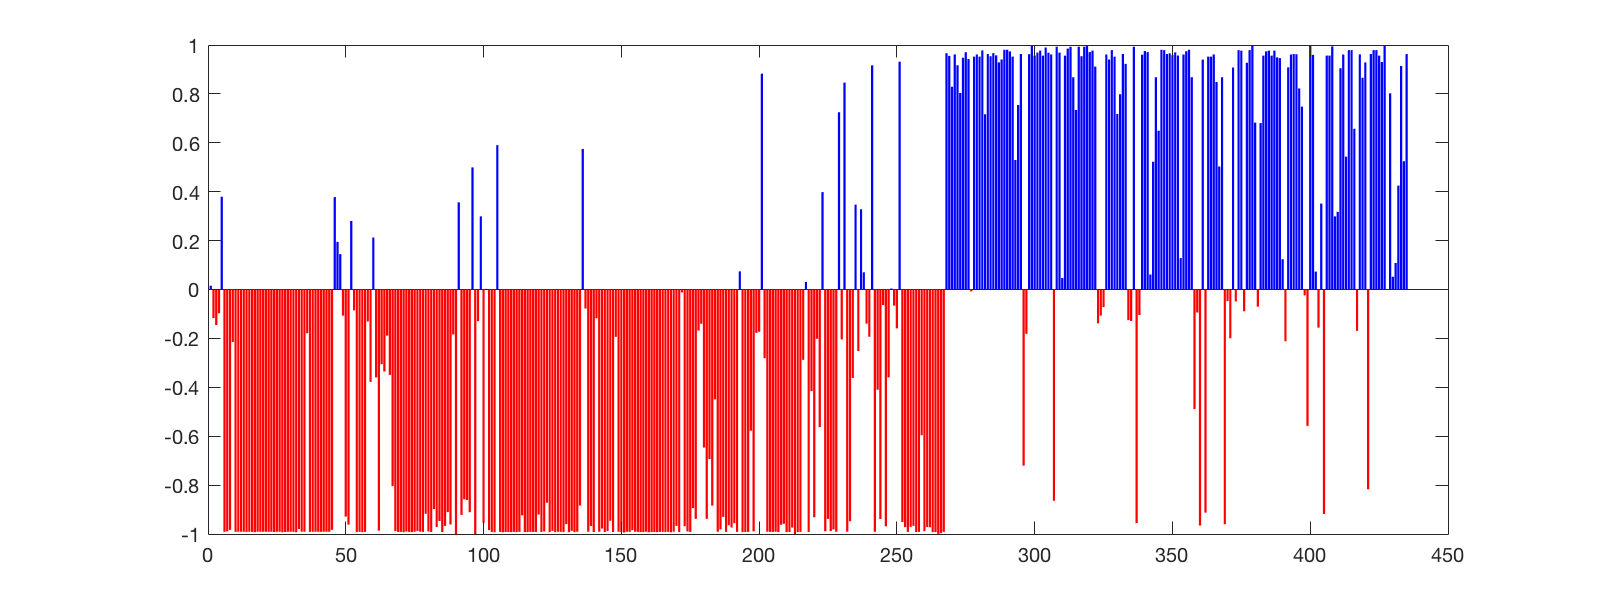
\includegraphics[width=\linewidth]{learnM/voting/hier/u_avg.png}
            \end{minipage} \hfill
            \begin{minipage}{0.48\textwidth}
                \centering
                \caption{\label{fig:voting_hier_xi_M_accept} \cref{alg:hier_t_a_M}, $M$ and $\xi$ acceptance probabilities}
                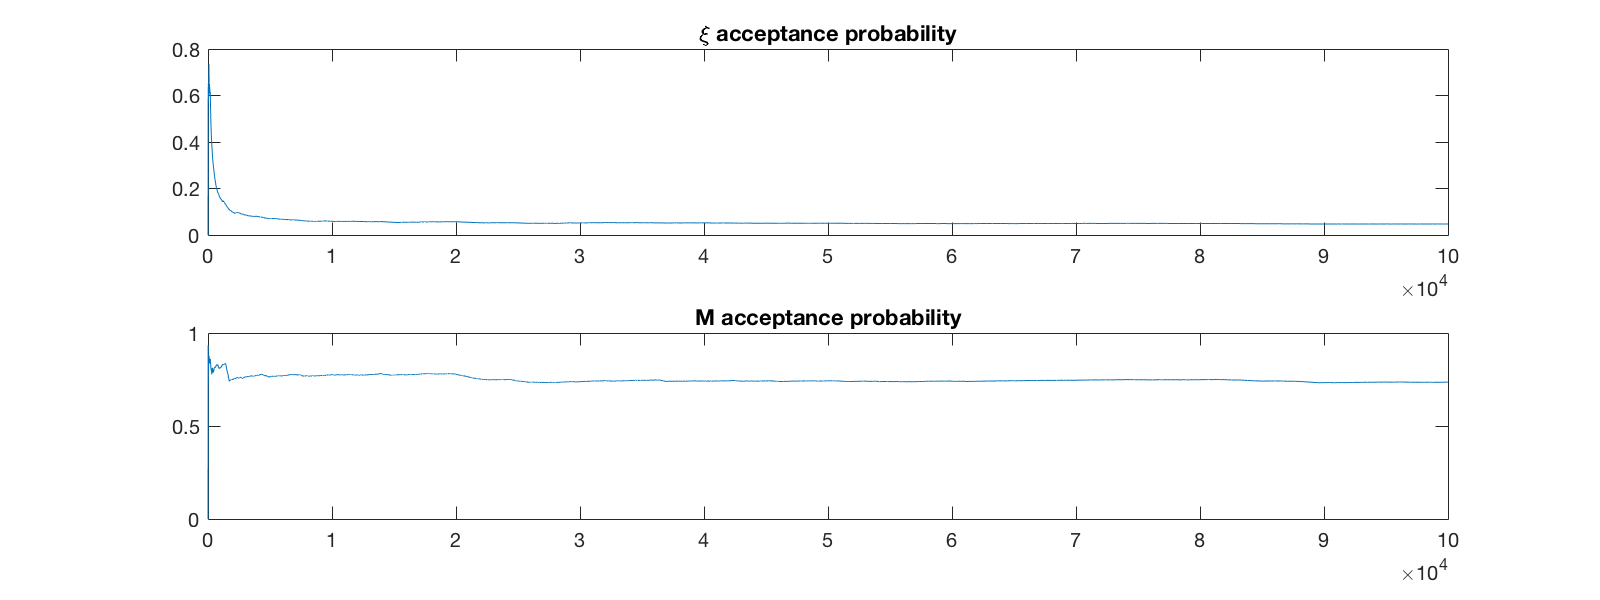
\includegraphics[width=\linewidth]{learnM/voting/hier/accept_prob.png}
            \end{minipage}
            \end{figure}

            \begin{figure}[!htb]
            \begin{minipage}{0.48\textwidth}
                \centering
                \caption{\label{fig:voting_hier_eigenvector} 34th eigenvector of unnormalized fixed length-scale $L$}
                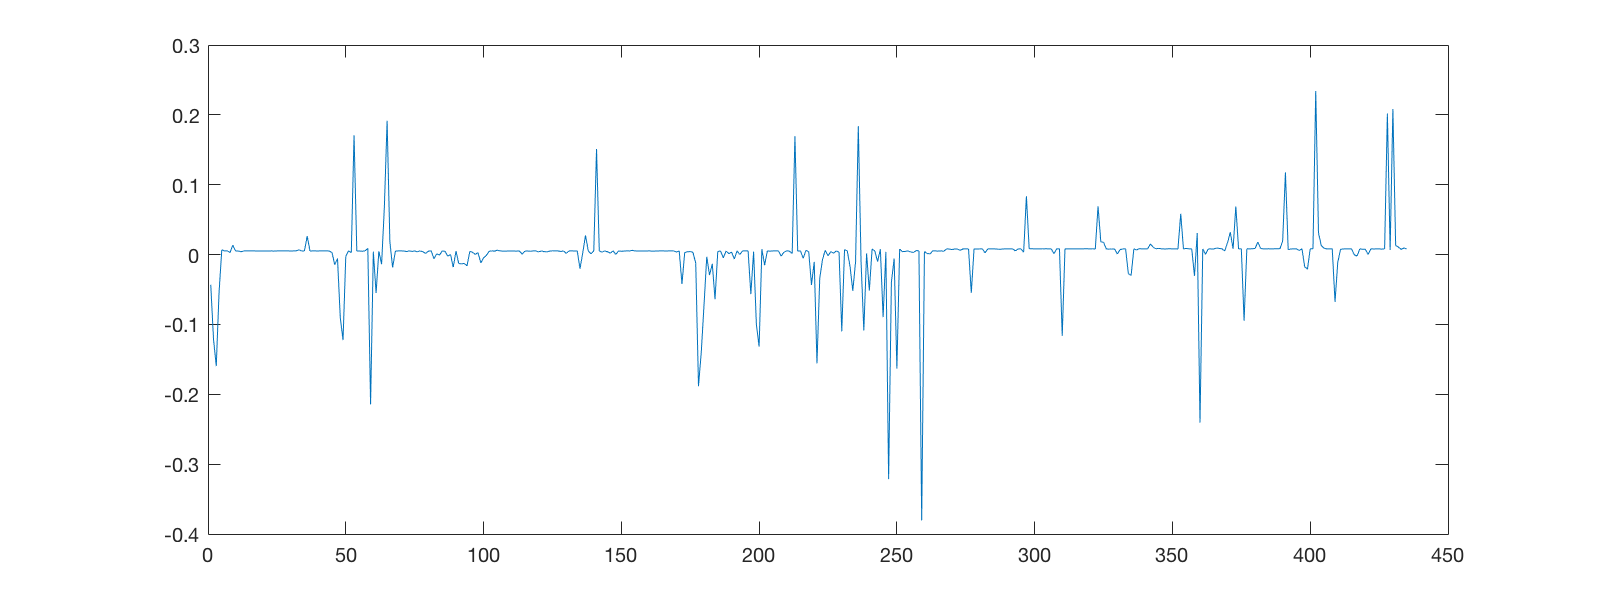
\includegraphics[width=\linewidth]{learnM/voting/hier/34_eigvec.png}
            \end{minipage}\hfill
            \begin{minipage}{0.48\textwidth}
                \centering
                \caption{\label{fig:voting_hier_M_trace} \cref{alg:hier_t_a_M}, trace of $M$}
                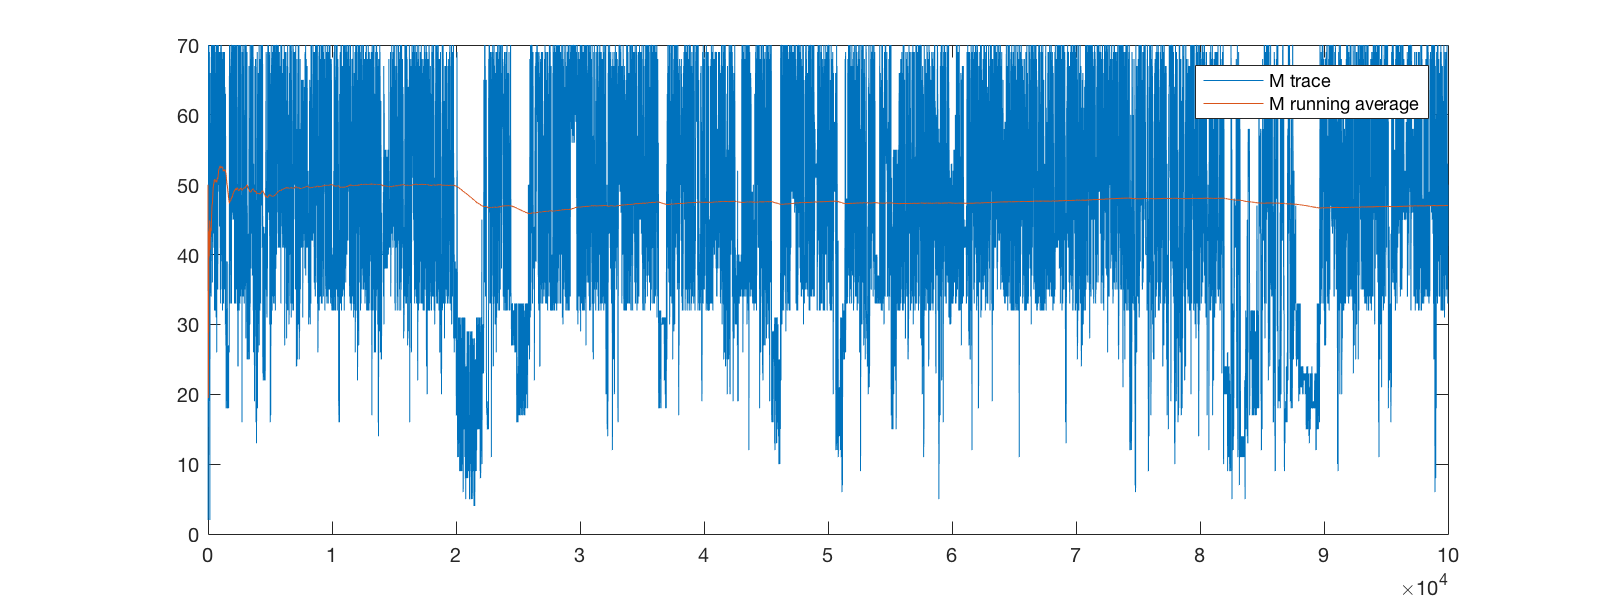
\includegraphics[width=\linewidth]{learnM/voting/hier/M_trace.png}
            \end{minipage}
            \end{figure}


        \subsubsection{Two moons}
            I tried a similar set of experiments on the two moons data. I fixed $\tau = 2, \alpha = 35$, again following the expected values of these hyperparameters from the noncentered algorithm that learns $\tau,\alpha$. I set the pCN to use the first $100$ eigenvectors, and I set the range for $M$ in \cref{alg:hier_t_a_M} to be $[1, 70]$. The two moons data was generated with $N=2000, d=100, \sigma = 0.2$ and $1\%$ fidelity. The nodes selected for fidelity are random but consistent between the different methods, as is the data itself. The colored diamonds in the scatter plots are the labeled nodes.

            One realization of this test is shown in \cref{fig:moons_nonhier_scatter}, \cref{fig:moons_nonhier_u_accept} for pCN, and \cref{fig:moons_hier_scatter}, \cref{fig:moons_hier_M_xi_accept}, \cref{fig:moons_hier_M_trace} for the hierarchical algorithm.  In this particular realization, the two algorithms performed similarly, with $90.56\%$ accuracy for pCN and $91.97\%$ accuracy for the hierarchical algorithm as shown in the final clusterings in \cref{fig:moons_nonhier_scatter} and \cref{fig:moons_hier_scatter}. In \cref{fig:moons_hier_M_trace}, $M$ seems to have moved from its uniform prior distribution, preferring a mean of around $20$. The results again suggest that there is some value to being hierarchical with $M$ even with good choices of $\tau$ and $\alpha$, but more experiments are needed. 


            \begin{figure}[!htb]
            \begin{minipage}{0.48\textwidth}
                \centering
                \caption{\label{fig:moons_nonhier_scatter} pCN, final classification projected into first two dimensions.}
                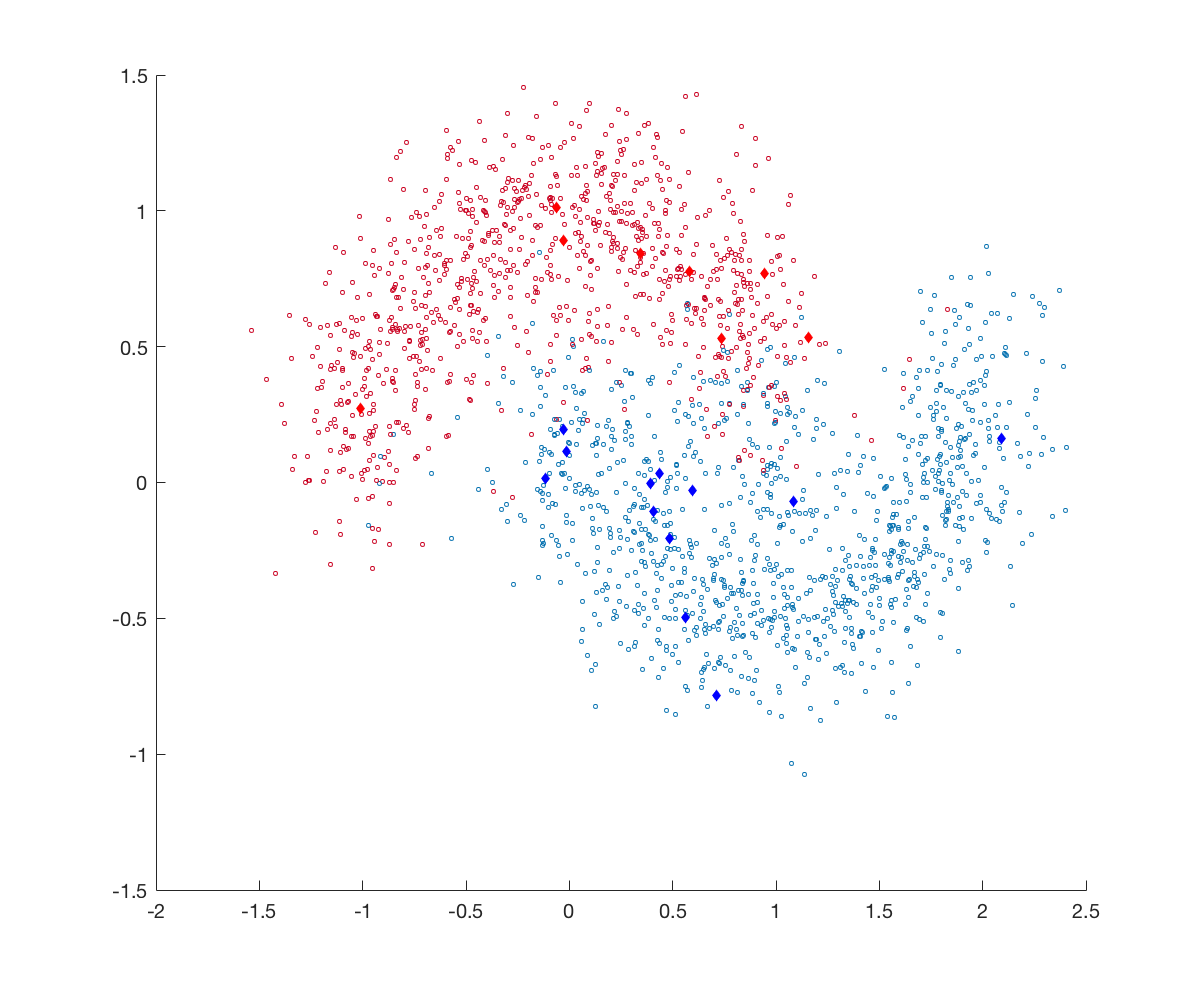
\includegraphics[width=\linewidth]{learnM/moons/nonhier/sigma_0_20/scatter.png}
            \end{minipage} \hfill
            \begin{minipage}{0.48\textwidth}
                \centering
                \caption{\label{fig:moons_nonhier_u_accept} pCN, $u$ acceptance probability.}
                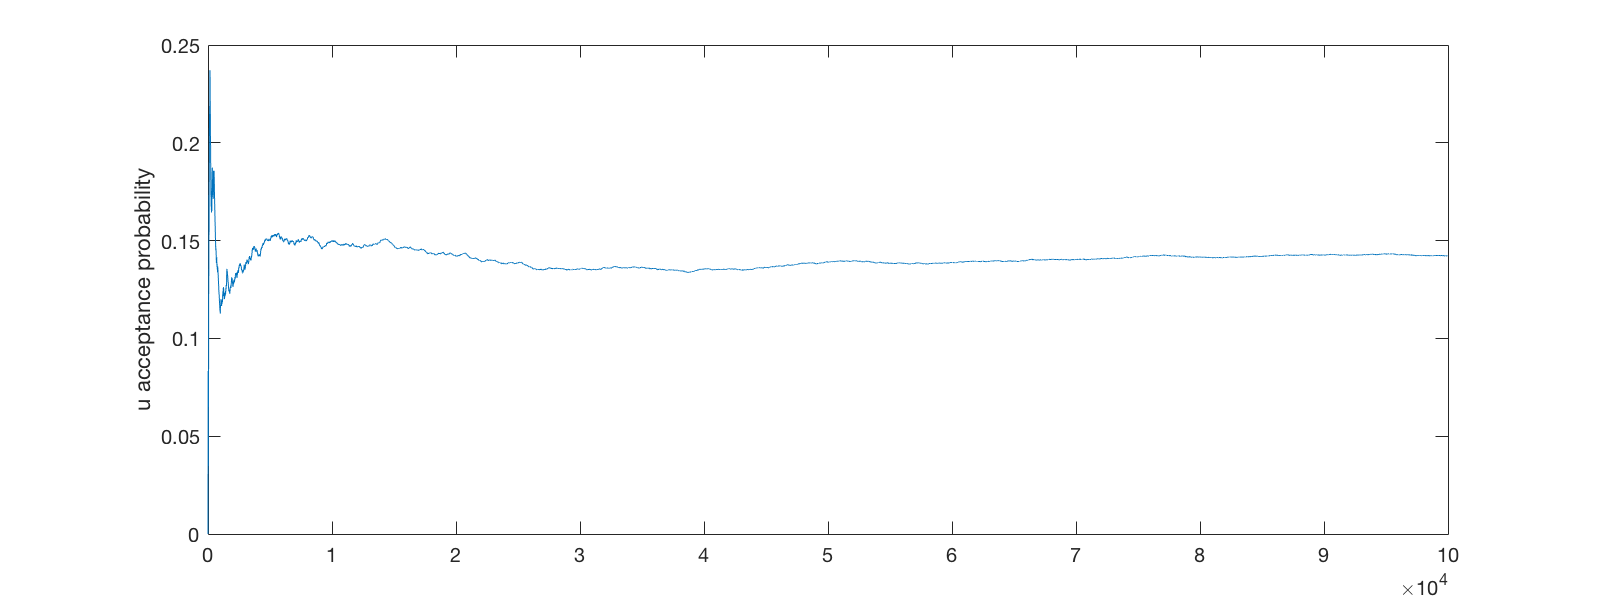
\includegraphics[width=\linewidth]{learnM/moons/nonhier/sigma_0_20/u_accept.png}
            \end{minipage}
            \end{figure}

            \begin{figure}[!htb]
            \begin{minipage}{0.48\textwidth}
                \centering
                \caption{\label{fig:moons_hier_scatter} Hierarchical, final classification projected into first two dimensions.}
                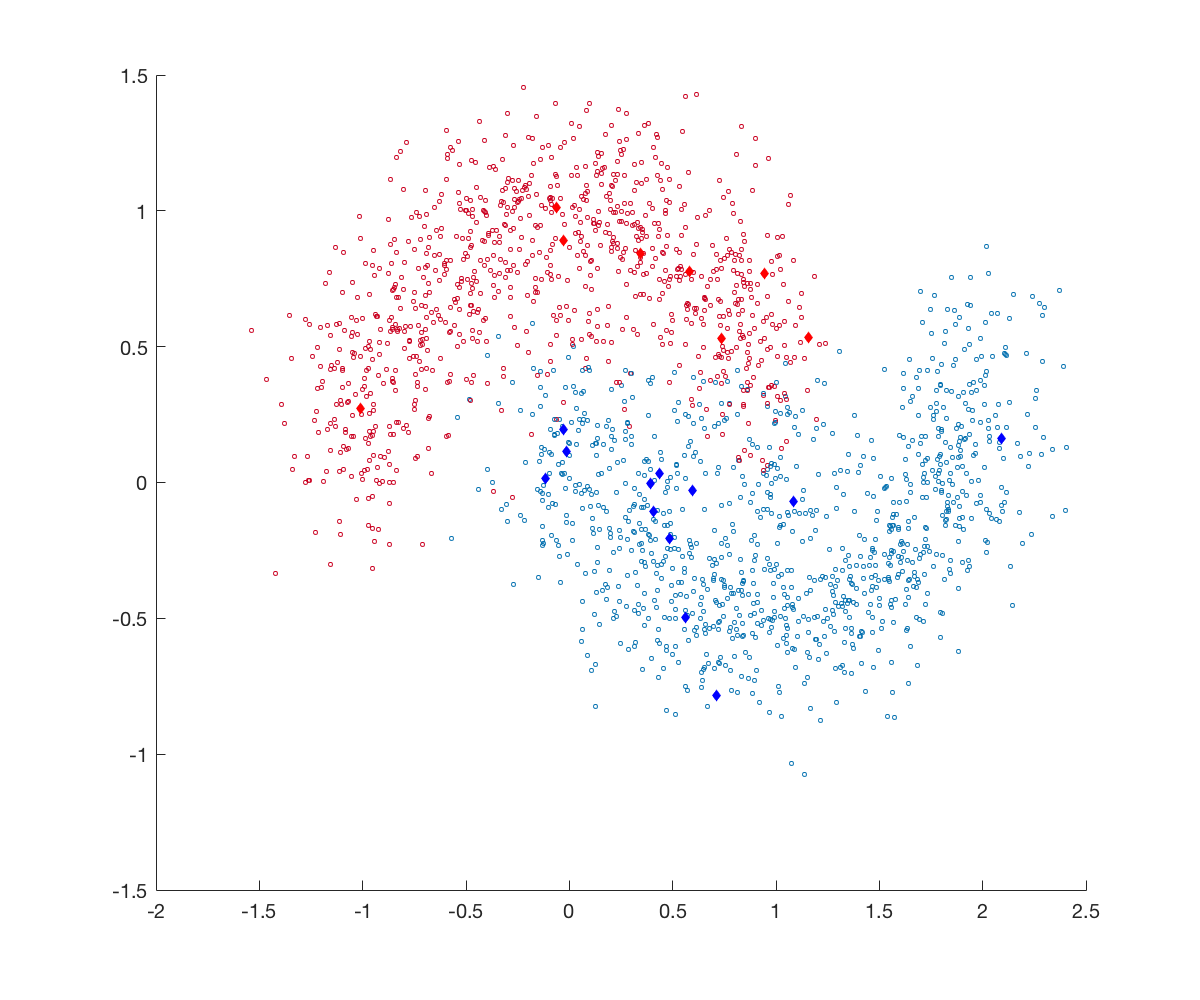
\includegraphics[width=\linewidth]{learnM/moons/hier/sigma_0_20/scatter.png}
            \end{minipage} \hfill
            \begin{minipage}{0.48\textwidth}
                \centering
                \caption{\label{fig:moons_hier_M_xi_accept} Hierarchical, $\xi$ acceptance probability.}
                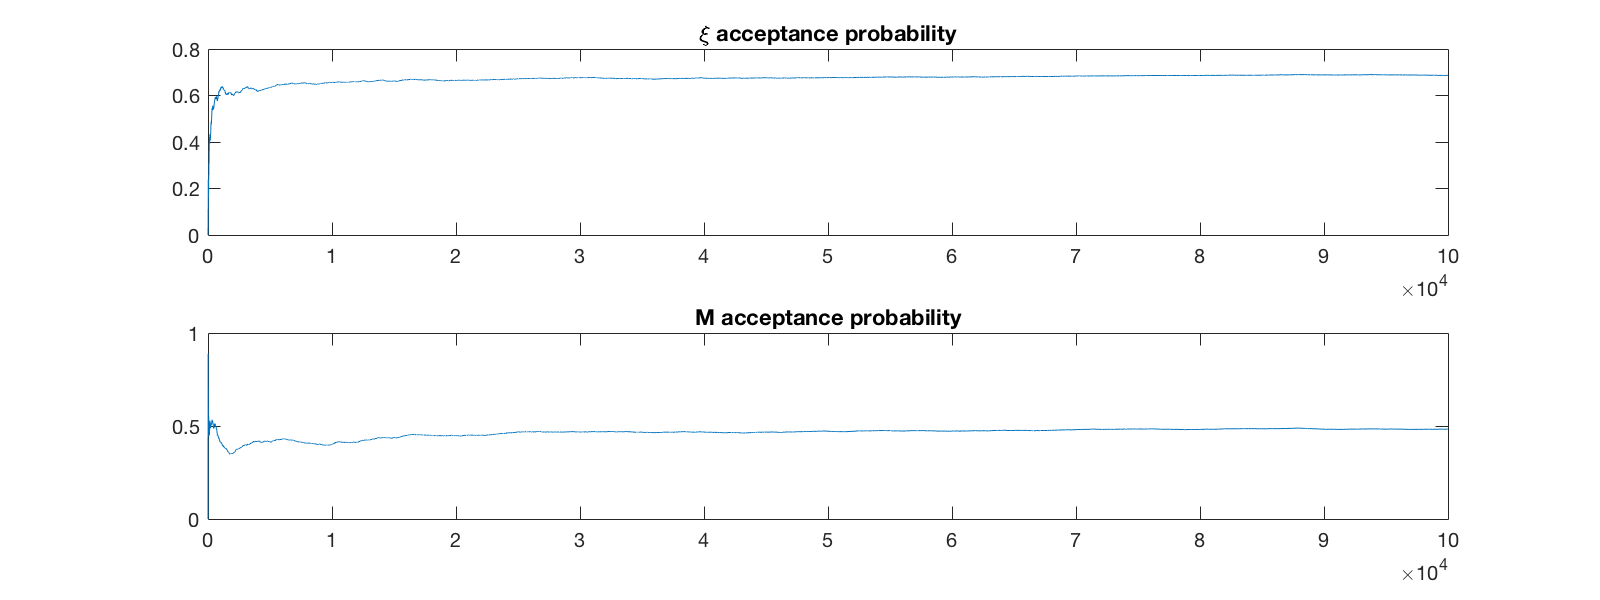
\includegraphics[width=\linewidth]{learnM/moons/hier/sigma_0_20/accept_prob.png}
            \end{minipage}
            \end{figure}

            \begin{figure}[!htb]
                \centering
                \caption{\label{fig:moons_hier_M_trace} Hierarchical, seed $\text{rng}(3)$. $M$ trace.}
                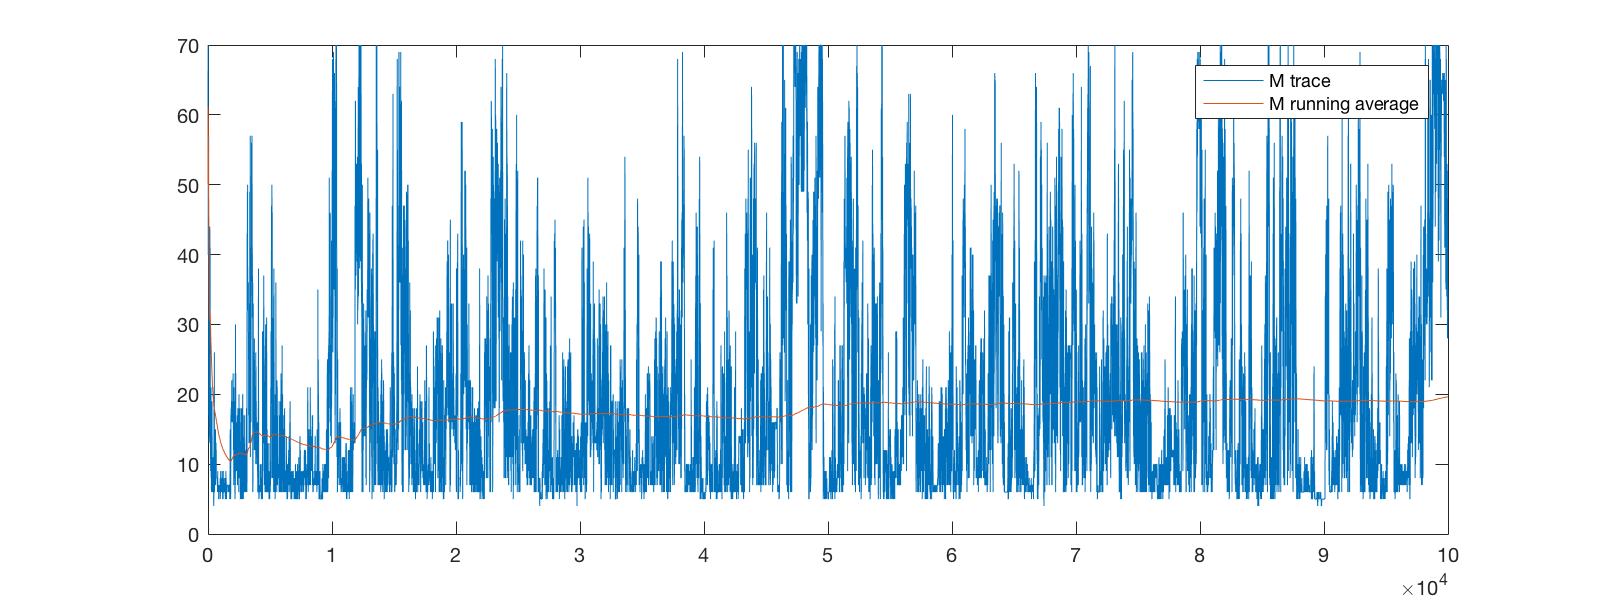
\includegraphics[width=0.6\linewidth]{learnM/moons/hier/sigma_0_20/M_trace.png}
            \end{figure}

\section{Experiments with model (E)}
    We run some experiments with \cref{alg:hier_v_M}, model (E), on the two moons dataset. We again fix $\tau = 2, \alpha = 35$, and pick $a=0.5$ to create the prior on $v$. We pick the walk size for $v$ to be $\epsilon = 1.0\times 10^{-13}$. We allow the prior on $M$ to be uniform, $\mathsf{U}(1,70)$. If we compare this algorithm against model (C) with fixed $\tau, \alpha$, this is equivalent to setting $\epsilon = 0$ and fixing $v$ to be at the mean of its prior. Learning $v$ and $M$ does not seem to greatly affect the classification accuracy compared to just learning $M$. Consider the following run on two moons, with fidelity = 1\%, $\sigma = 0.2$, in \cref{fig:modelE_learn_v} and \cref{fig:modelE_fixed_v}. The model that learns $v, M$ obtained $85.45\%$ accuracy while the one that only learns $M$ obtained $86.52\%$ accuracy. The histograms of $M$ appear very similar, with the same cutoff observed at the $14$th index. The average values of the $u_j$ coefficients also seem to agree in magnitude and sign between the two algorithms.

    \begin{figure}
        \caption{\label{fig:modelE_learn_v}Learning $v, M$. The bottom left figure was one observation of the $v_j$.}
        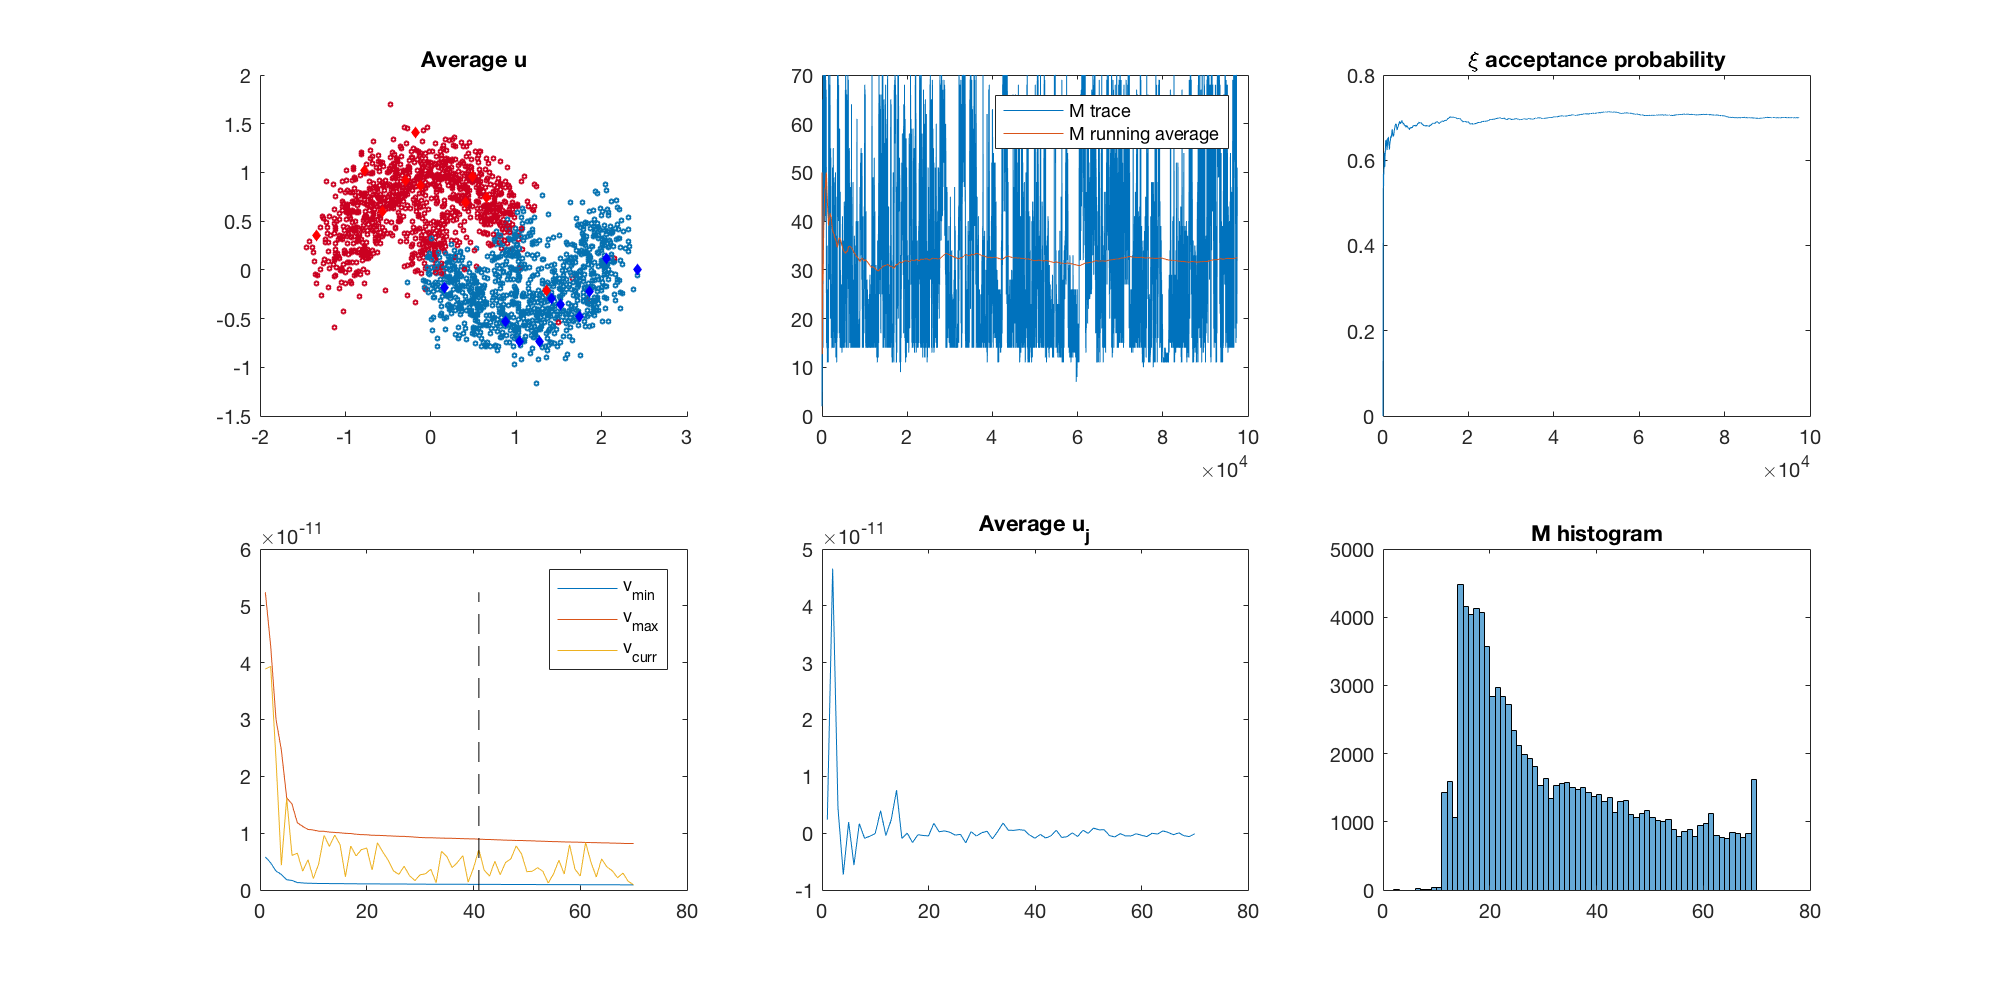
\includegraphics[width=\linewidth]{learnv/v_uniform_prior/all.png}
    \end{figure}

    \begin{figure}
        \caption{\label{fig:modelE_fixed_v}Learning only $M$}
        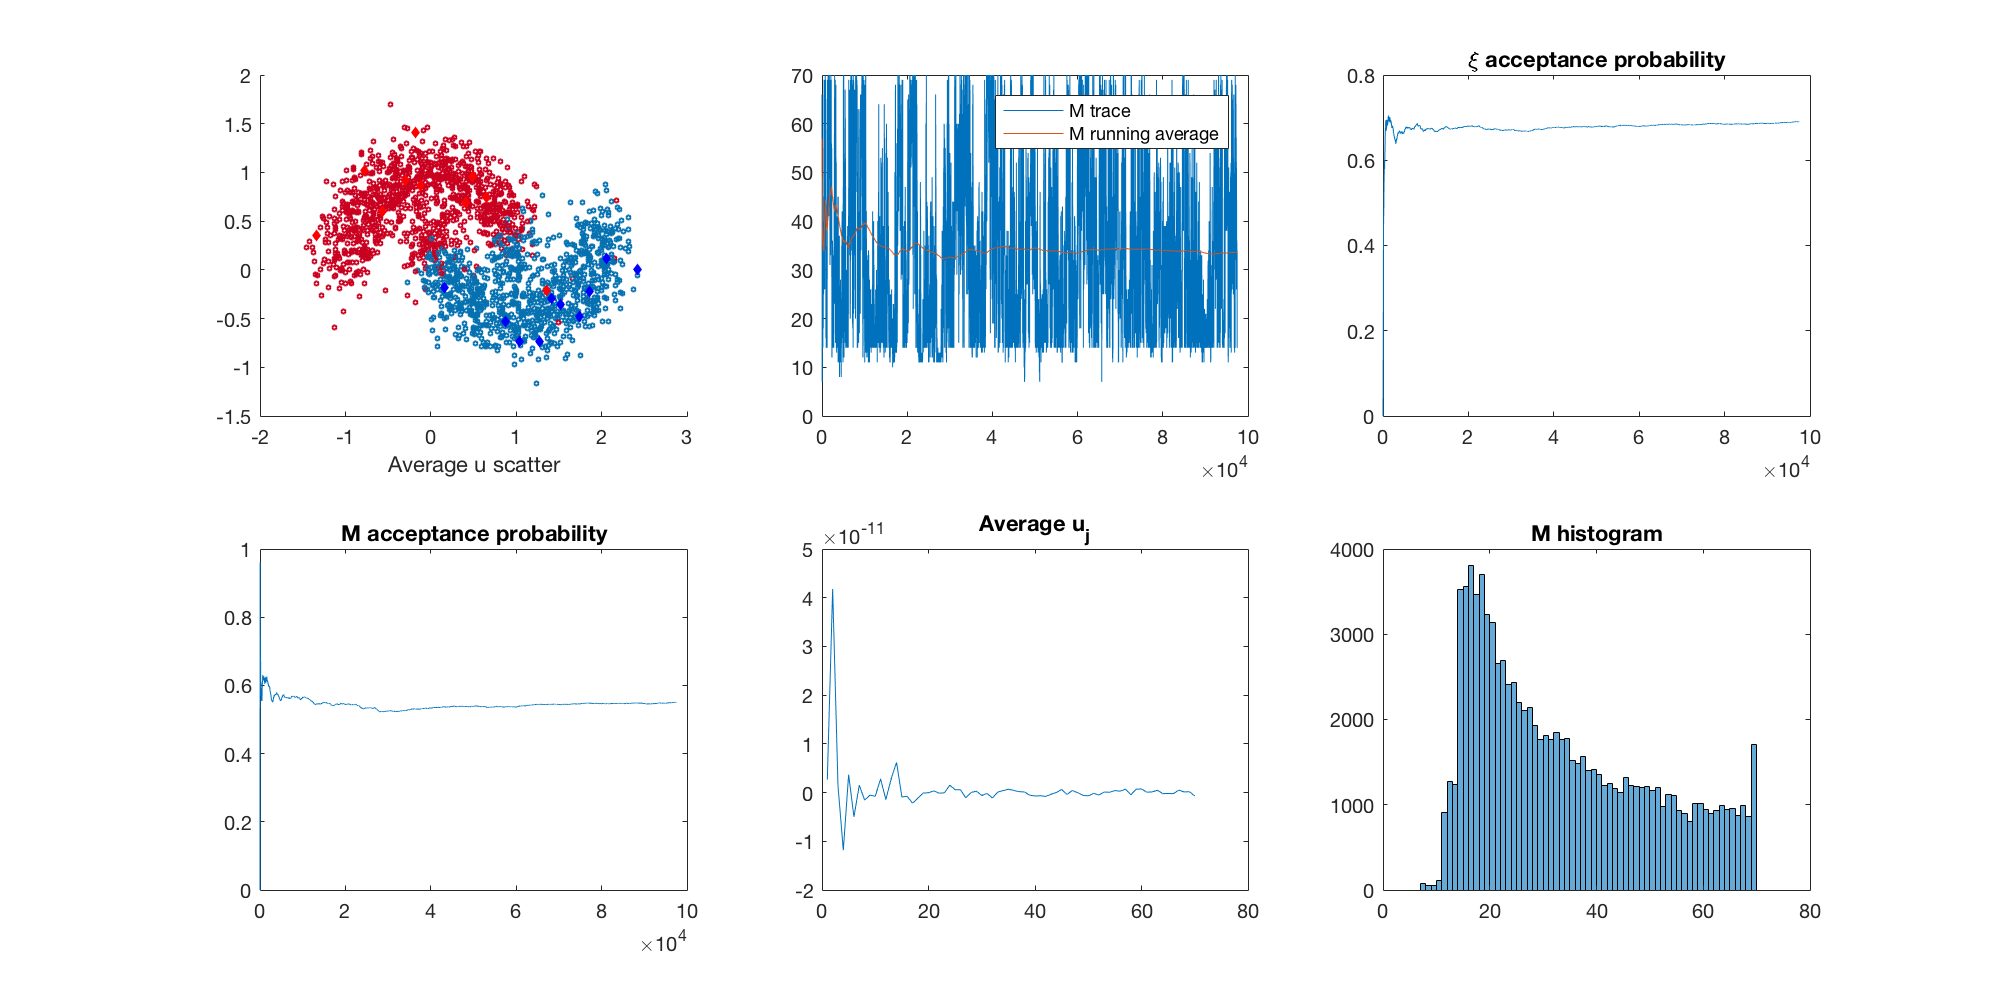
\includegraphics[width=\linewidth]{learnv/v_fixed/all.png}
    \end{figure}
    
\section{Multiclass experiments} \label{sec:Multiclass experiments}
    We use the MNIST dataset and attempt to cluster $k$ different digits. We want to compare the algorithm that learns $\tau, \alpha$ against the nonhierarchical algorithm with fixed $\tau, \alpha$, so we fix $\tau=2, \alpha=35$ for the nohierarchical algorithm and initialize $\tau=2, \alpha=35$ for the hierarchical algorithm. Additionally, for the hierarchical algorithm we currently restrict $(\tau,\alpha)$ to be the same for each of the $k$ priors. We fix $\gamma = 0.1, \beta = 0.1$ for both algorithms. We test on the digits $[1, 4, 9]$ with the same $1\%$ fidelity selected between the two trials. The final classification is given by $S(\mathbb{E}(S(u)))$, with a burn-in of 5000 and 100000 total iterations. The hierarchical algorithm obtained $94.33\%$ accuracy while the nonhierarchical algorithm obtained $88.67\%$. This observation supports the claim that there is value in learning $\tau, \alpha$. See \cref{fig:multiclass_nonhier_table}, \cref{fig:multiclass_nonhier_accept}, \cref{fig:multiclass_hier_t_a_same_table}, \cref{fig:multiclass_hier_t_a_same_accept}, \cref{fig:multiclass_hier_t_a_same_trace}.

    Using $S(\mathbb{E}(S(u)))$ seems to give a better accuracy for the hierarchical algorithm than $S(\mathbb{E}(u))$, which would only obtain $88.62\%$ accuracy for the above example. This seems to have to do with the high variance in the scale of $u$, which allows a few observations to dominate the classification. However, the choice of $S(\mathbb{E}(u))$ is more natural perhaps, since $\mathbb{E}(u)$ is the expected value of $u$ in the posterior distribution.

    \begin{figure}[!htb]
        \begin{minipage}{0.48\textwidth}
            \centering
            \caption{\label{fig:multiclass_nonhier_table} Nonhierarchical multiclass $[1, 4, 9]$, final classification}
            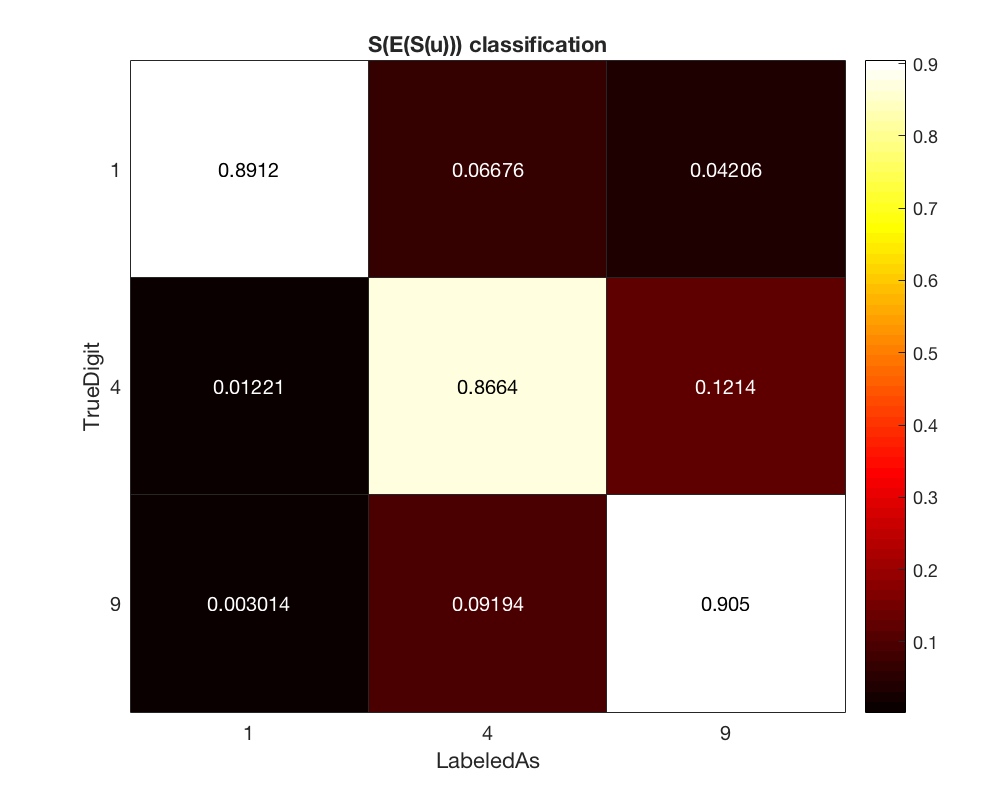
\includegraphics[width=\linewidth]{multiclass/nonhier/table.png}
        \end{minipage}\hfill
        \begin{minipage}{0.48\textwidth}
            \centering
            \caption{\label{fig:multiclass_nonhier_accept} Nonhierarchical multiclass $[1, 4, 9]$, $\xi$ acceptance probability}
            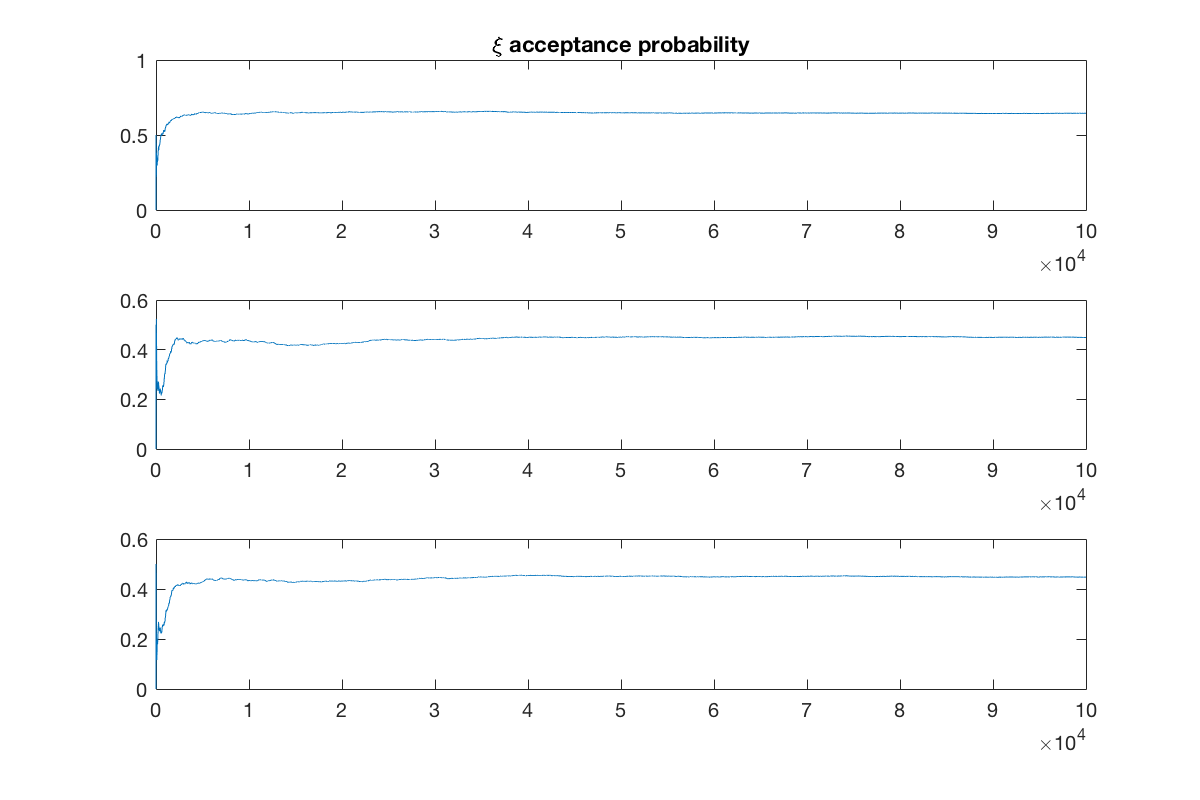
\includegraphics[width=\linewidth]{multiclass/nonhier/xi_accept.png}
        \end{minipage}
    \end{figure}

    \begin{figure}[!htb]
        \begin{minipage}{0.48\textwidth}
            \centering
            \caption{\label{fig:multiclass_hier_t_a_same_table} Hierarchical multiclass $[1, 4, 9]$, final classification}
            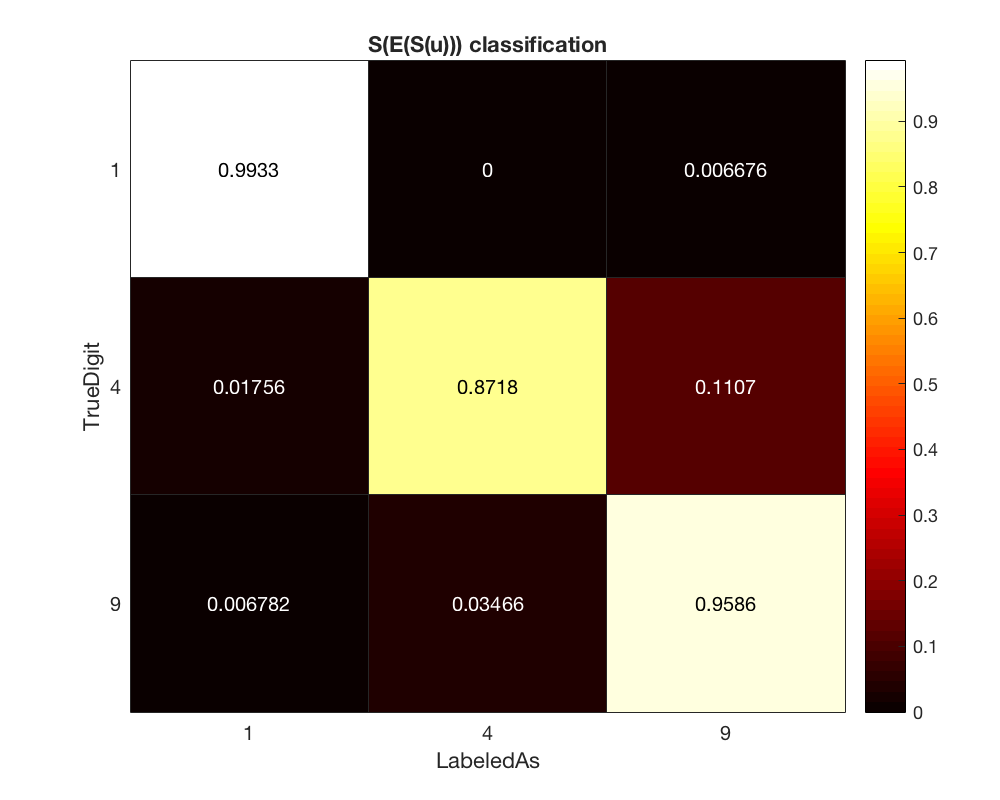
\includegraphics[width=\linewidth]{multiclass/hier_t_a_same/table.png}
        \end{minipage}\hfill
        \begin{minipage}{0.48\textwidth}
            \centering
            \caption{\label{fig:multiclass_hier_t_a_same_accept} Hierarchical multiclass $[1, 4, 9]$, $\xi$ acceptance probability}
            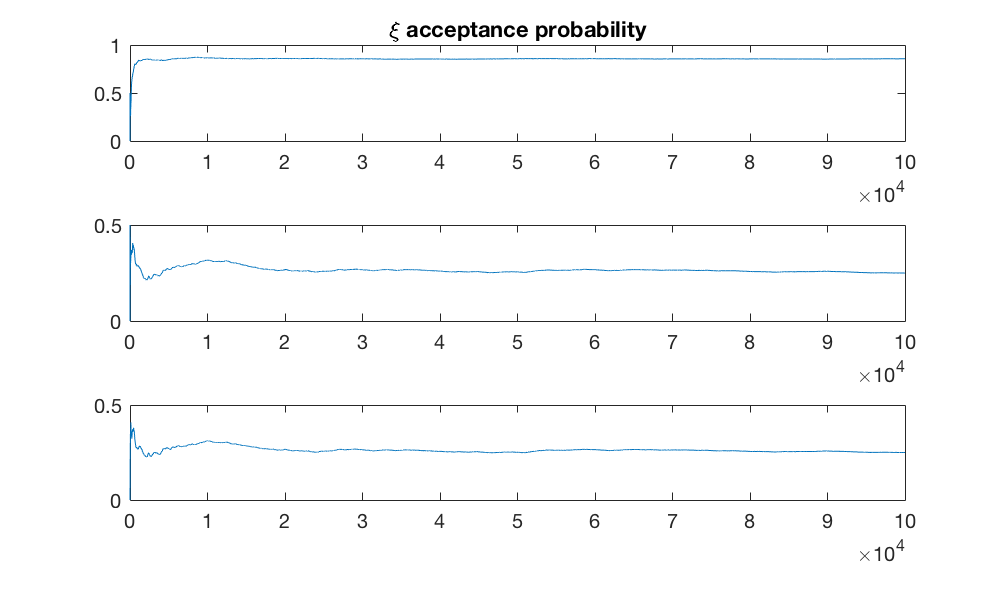
\includegraphics[width=\linewidth]{multiclass/hier_t_a_same/xi_accept.png}
        \end{minipage}
    \end{figure}

    \begin{figure}[!htb]
        \centering
        \caption{\label{fig:multiclass_hier_t_a_same_trace} Hierarchical multiclass $[1, 4, 9]$, $\tau$ and $\alpha$ traces}
        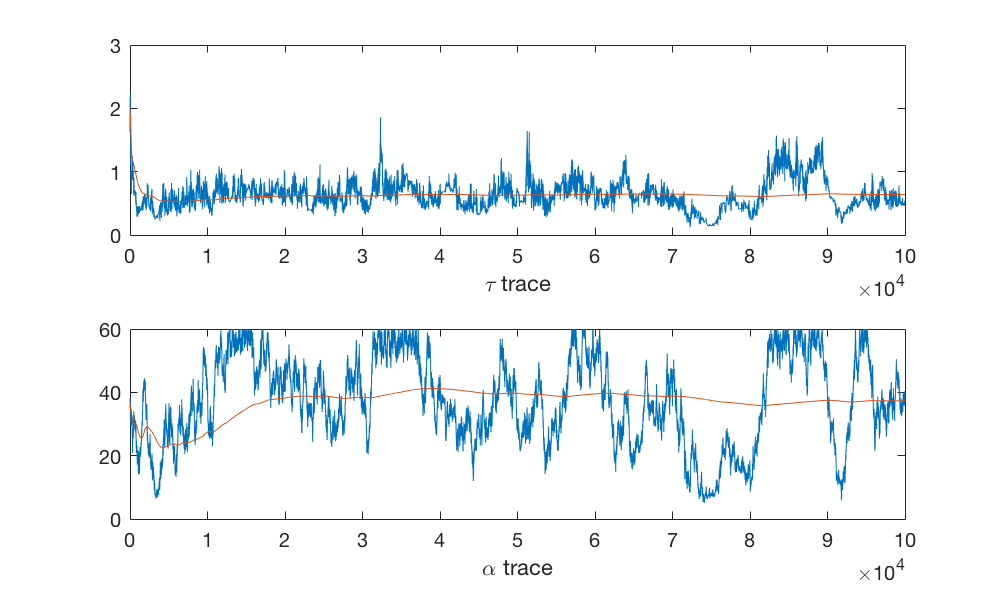
\includegraphics[width=0.8\linewidth]{multiclass/hier_t_a_same/a_t_trace.png}
    \end{figure}

    \begin{figure}[!htb]
        \centering
        \caption{\label{fig:multiclass_hier_t_a_same_learn_t} Hierarchical multiclass $[1, 4, 9]$, $\tau_0 = 20$ and learning $\tau$}
        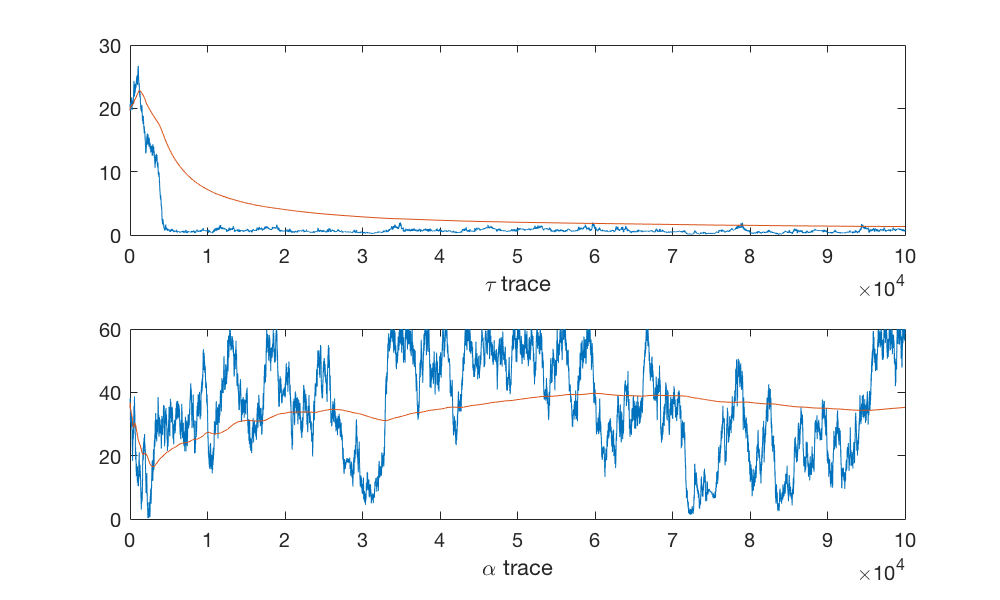
\includegraphics[width=0.8\linewidth]{multiclass/learn_t/trace.png}
    \end{figure}
    We can also see the same behavior with $\tau$ that we observed in the binary case. Initializing $\tau = 20$ and $\alpha = 35$ in \cref{fig:multiclass_hier_t_a_same_learn_t}, we can see that $\tau$ learns that it should be small, averaging around $0.6$. This value seems pretty consistent across different initial values of $\tau$. We can also see that there is strong correlation between $\tau$ and $\alpha$, for instance by visually matching the extrema in \cref{fig:multiclass_hier_t_a_same_trace}.

\section{Challenges}
    One problem I have been running into is that these MCMC simulations take a while to run. Since a large number of iterations is needed to ensure convergence and there is matrix multiplication for converting from eigenbasis to standard basis, large test suites are time consuming. My workaround for this problem is to run these tests overnight and analyze the results in the morning.

    Another problem I encountered was the difference between $S(\mathbb{E}(S(u)))$ and $S(\mathbb{E}(u))$ as the choice of the classifying function. While $S(\mathbb{E}(u))$ is more natural as discussed in \cref{sec:Multiclass experiments}, this allows large $u$ to dominate the entire classification, and large $u$ can arise when $\tau$ is small, $\alpha$ is large, and the choice is accepted. I noticed this issue when I saw that the classification sometimes would get stuck at a percentage with little change for the remaining iterations. My solution has been to use $S(\mathbb{E}(S(u)))$ for now, and it seems to give better classification.
    
\section{Goals}
    One research goal for the remainder of the summer is to gather more data comparing the algorithm that learns $M$ against the nonhierarchical algorithm to determine if the method is beneficial. It will also be interesting to better analyze the relationship between $\sigma$ and $M$ in the two moons dataset. Preliminary experiments suggest that in low $\sigma$ data, small $M$ is enough for an accurate clustering, but in large $\sigma$, higher $M$ is necessary as more eigenvectors are needed to fit the problem. It could be interesting to create a plot of average $M$ versus increasing $\sigma$ to test this hypothesis. \\
    Also, I hope to look at different prior choices for $v$ for \cref{alg:hier_v} and \cref{alg:hier_v_M}. It appears that learning $v_j$ and $M$ with a uniform prior on $v_j$ is similar to just learning $M$, so a different prior choice could be useful. For example, one idea is to define $l_j = \frac{1}{v_j^2}$ and assume a gamma distribution for $l_j$ with shape depending on $j$. \\
    Another goal is to study different multiclass hierarchical methods and implement a multiclass algorithm that learns $M$. I am working on implementing the different choices described in \cref{sec:algorithms_multiclass}. In particular, independently evolving hyperparameters $\tau, \alpha, M$ for each of the $k$ priors should be studied.

\bibliographystyle{siamplain}
\bibliography{references}
\end{document}